% Options for packages loaded elsewhere
\PassOptionsToPackage{unicode}{hyperref}
\PassOptionsToPackage{hyphens}{url}
%
\documentclass[
  openany]{book}
\usepackage{amsmath,amssymb}
\usepackage{lmodern}
\usepackage{iftex}
\ifPDFTeX
  \usepackage[T1]{fontenc}
  \usepackage[utf8]{inputenc}
  \usepackage{textcomp} % provide euro and other symbols
\else % if luatex or xetex
  \usepackage{unicode-math}
  \defaultfontfeatures{Scale=MatchLowercase}
  \defaultfontfeatures[\rmfamily]{Ligatures=TeX,Scale=1}
\fi
% Use upquote if available, for straight quotes in verbatim environments
\IfFileExists{upquote.sty}{\usepackage{upquote}}{}
\IfFileExists{microtype.sty}{% use microtype if available
  \usepackage[]{microtype}
  \UseMicrotypeSet[protrusion]{basicmath} % disable protrusion for tt fonts
}{}
\makeatletter
\@ifundefined{KOMAClassName}{% if non-KOMA class
  \IfFileExists{parskip.sty}{%
    \usepackage{parskip}
  }{% else
    \setlength{\parindent}{0pt}
    \setlength{\parskip}{6pt plus 2pt minus 1pt}}
}{% if KOMA class
  \KOMAoptions{parskip=half}}
\makeatother
\usepackage{xcolor}
\IfFileExists{xurl.sty}{\usepackage{xurl}}{} % add URL line breaks if available
\IfFileExists{bookmark.sty}{\usepackage{bookmark}}{\usepackage{hyperref}}
\hypersetup{
  pdftitle={Documento Técnico N°5: Medición de la contribución económica del turismo},
  pdfauthor={Dirección Nacional de Mercados y Estadísticas - Subsecretaría de Desarrollo Estratégico},
  hidelinks,
  pdfcreator={LaTeX via pandoc}}
\urlstyle{same} % disable monospaced font for URLs
\usepackage{longtable,booktabs,array}
\usepackage{calc} % for calculating minipage widths
% Correct order of tables after \paragraph or \subparagraph
\usepackage{etoolbox}
\makeatletter
\patchcmd\longtable{\par}{\if@noskipsec\mbox{}\fi\par}{}{}
\makeatother
% Allow footnotes in longtable head/foot
\IfFileExists{footnotehyper.sty}{\usepackage{footnotehyper}}{\usepackage{footnote}}
\makesavenoteenv{longtable}
\usepackage{graphicx}
\makeatletter
\def\maxwidth{\ifdim\Gin@nat@width>\linewidth\linewidth\else\Gin@nat@width\fi}
\def\maxheight{\ifdim\Gin@nat@height>\textheight\textheight\else\Gin@nat@height\fi}
\makeatother
% Scale images if necessary, so that they will not overflow the page
% margins by default, and it is still possible to overwrite the defaults
% using explicit options in \includegraphics[width, height, ...]{}
\setkeys{Gin}{width=\maxwidth,height=\maxheight,keepaspectratio}
% Set default figure placement to htbp
\makeatletter
\def\fps@figure{htbp}
\makeatother
\setlength{\emergencystretch}{3em} % prevent overfull lines
\providecommand{\tightlist}{%
  \setlength{\itemsep}{0pt}\setlength{\parskip}{0pt}}
\setcounter{secnumdepth}{5}
  %%% REFERENCIAS
        \usepackage{hyperref}
        % links del indice en negro; citas y URL en azul
        \hypersetup{colorlinks = true, urlcolor={blue}, 
        citecolor={blue}, linkcolor ={blue}}
\usepackage[spanish]{babel} % Idiomas en los que se escribe el documento. 
\usepackage{booktabs}
\usepackage{amsthm}

\usepackage[final]{pdfpages}

\makeatletter
\def\thm@space@setup{%
  \thm@preskip=8pt plus 2pt minus 4pt
  \thm@postskip=\thm@preskip
}
\makeatother
\let\oldmaketitle\maketitle
\AtBeginDocument{\let\maketitle\relax}
\ifLuaTeX
  \usepackage{selnolig}  % disable illegal ligatures
\fi
\newlength{\cslhangindent}
\setlength{\cslhangindent}{1.5em}
\newlength{\csllabelwidth}
\setlength{\csllabelwidth}{3em}
\newenvironment{CSLReferences}[2] % #1 hanging-ident, #2 entry spacing
 {% don't indent paragraphs
  \setlength{\parindent}{0pt}
  % turn on hanging indent if param 1 is 1
  \ifodd #1 \everypar{\setlength{\hangindent}{\cslhangindent}}\ignorespaces\fi
  % set entry spacing
  \ifnum #2 > 0
  \setlength{\parskip}{#2\baselineskip}
  \fi
 }%
 {}
\usepackage{calc}
\newcommand{\CSLBlock}[1]{#1\hfill\break}
\newcommand{\CSLLeftMargin}[1]{\parbox[t]{\csllabelwidth}{#1}}
\newcommand{\CSLRightInline}[1]{\parbox[t]{\linewidth - \csllabelwidth}{#1}\break}
\newcommand{\CSLIndent}[1]{\hspace{\cslhangindent}#1}

\title{Documento Técnico N°5: Medición de la contribución económica del turismo}
\usepackage{etoolbox}
\makeatletter
\providecommand{\subtitle}[1]{% add subtitle to \maketitle
  \apptocmd{\@title}{\par {\large #1 \par}}{}{}
}
\makeatother
\subtitle{El turismo desde la perspectiva de la oferta: actividad y empleo}
\author{Dirección Nacional de Mercados y Estadísticas - Subsecretaría de Desarrollo Estratégico}
\date{05 de agosto de 2021}

\begin{document}
\maketitle

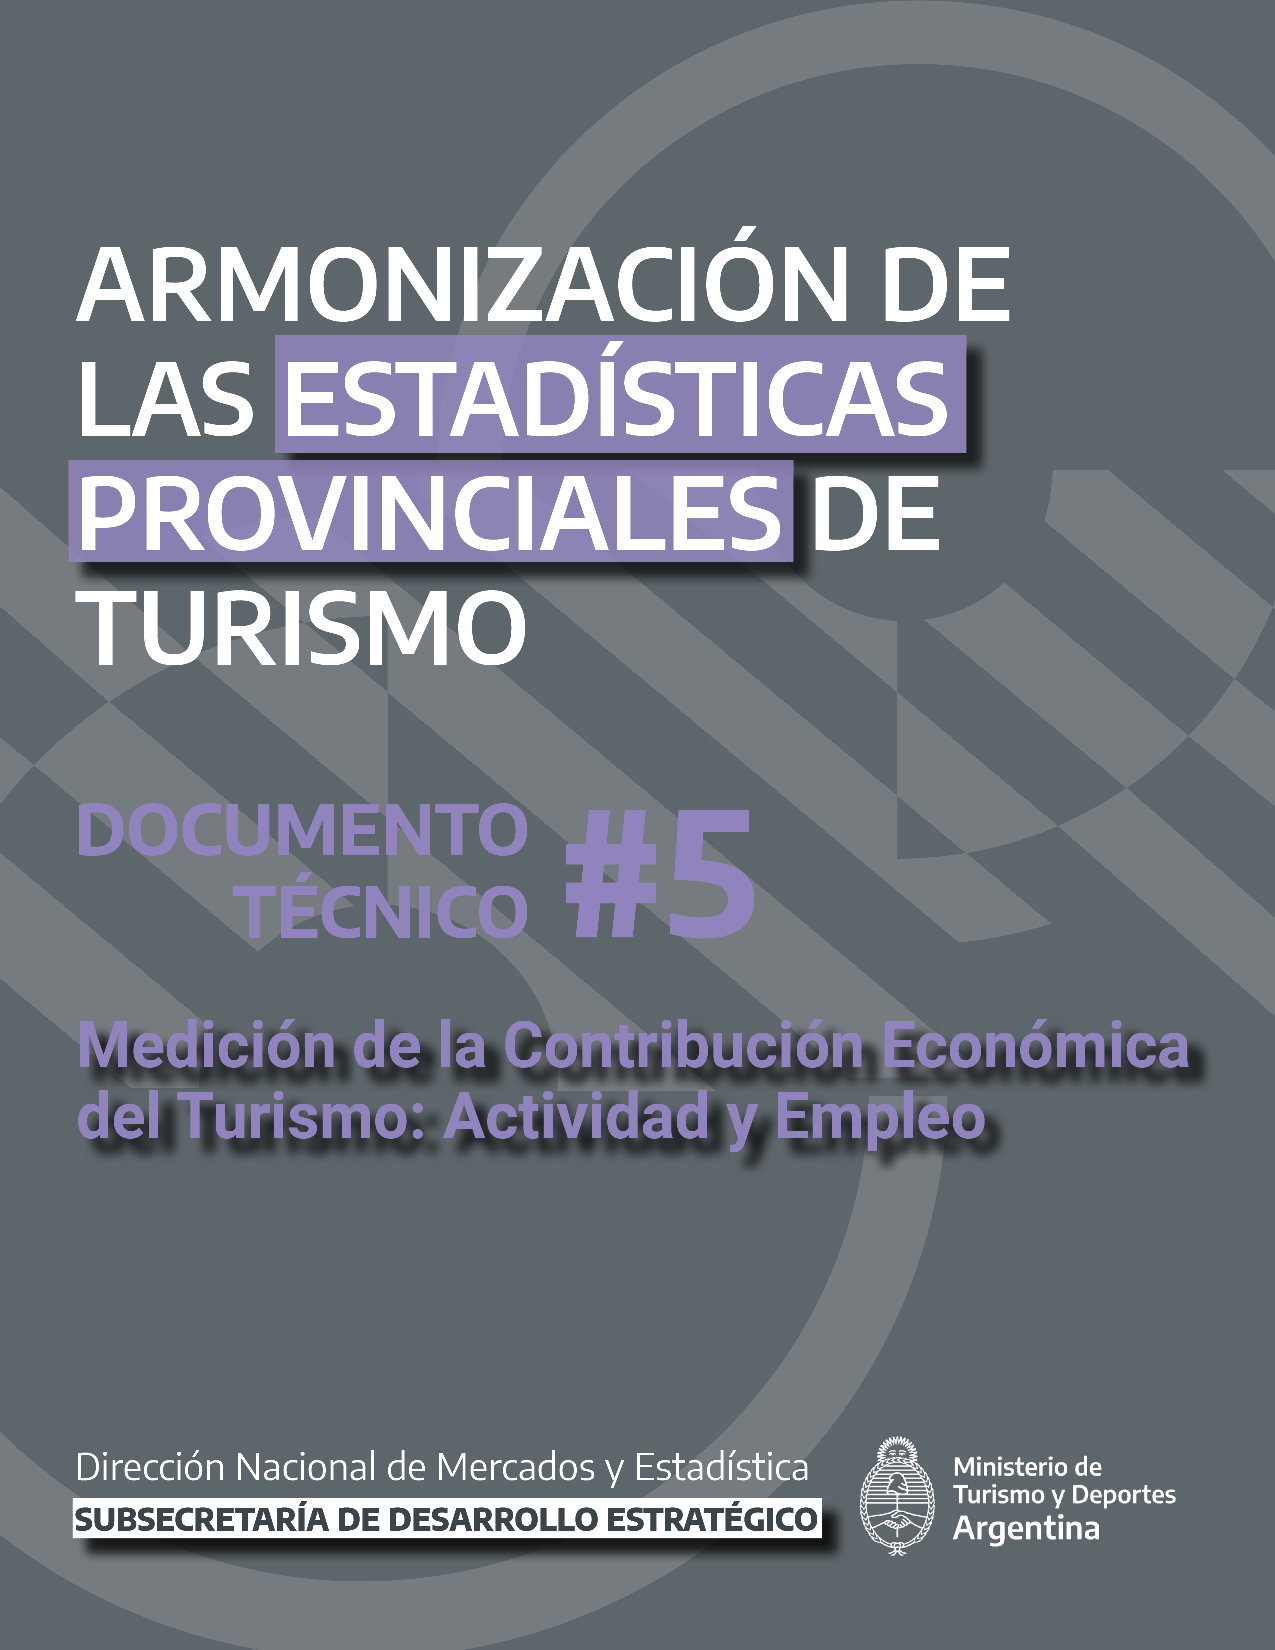
\includepdf[pages={1}, scale=1]{DT5Portada.pdf}
\newpage

\let\maketitle\oldmaketitle
\maketitle

{
\setcounter{tocdepth}{1}
\tableofcontents
}
\hypertarget{presentaciuxf3n}{%
\chapter*{Presentación}\label{presentaciuxf3n}}
\addcontentsline{toc}{chapter}{Presentación}

El presente documento, \textbf{Medición de la contribución económica del turismo: actividad y empleo}, se enmarca en el proyecto de Armonización de las Estadísticas de Turismo en las Provincias de la \href{https://www.yvera.tur.ar/estadistica/}{Dirección Nacional de Mercados y Estadística de la Subsecretaría de Desarrollo Estratégico del Ministerio de Turismo y Deportes}. El objetivo general de este proyecto es contribuir con propuestas metodológicas para los sistemas de estadísticas de turismo provinciales que orienten a producir indicadores provinciales básicos y comparables.

Además de este, se encuentra disponible una serie de documentos técnicos que abordan otras problemáticas vinculadas a la producción de estadística de turismo:

\begin{itemize}
\item
  \href{https://dnme-minturdep.github.io/DT1_medicion_turismo/}{Documento Técnico \#1}: Conceptos y elementos básicos para la medición provincial de los turistas
\item
  \href{https://dnme-minturdep.github.io/DT2_encuestas/}{Documento Técnico \#2}: Propuestas metodológicas para las encuestas de ocupación en alojamientos turísticos
\item
  \href{https://dnme-minturdep.github.io/DT3_registros_adminsitrativos/}{Documento Técnico \#3}: Descripción, análisis y utilización de los Registros Administrativos para la medición del Turismo
\item
  \href{https://dnme-minturdep.github.io/DT4_perfiles/}{Documento Técnico \#4}: Propuestas Metodológicas para las Encuestas de Perfil del Visitante
\end{itemize}

\hypertarget{documento-tuxe9cnico-nuxba5---resumen}{%
\subsection*{Documento Técnico Nº5 - Resumen}\label{documento-tuxe9cnico-nuxba5---resumen}}
\addcontentsline{toc}{subsection}{Documento Técnico Nº5 - Resumen}

El objetivo general es describir las metodologías disponibles para elaborar indicadores de la actividad del turismo desde la perspectiva de oferta. En particular se analizan los desafíos de la medición de la contribución económica del turismo a la actividad y el empleo desde las distintas ópticas territoriales. En virtud de estos objetivos, este documento se estructura en tres capítulos.

En el \textbf{Capítulo} \ref{medicion-actividad} se desarrolla una metodología, según las recomendaciones internacionales, para la medición de la contribución económica del turismo en un territorio. En sus diferentes secciones, presenta la definición y el alcance de las actividades económicas involucradas en el turismo a partir del enfoque de las Ramas Características, recomendaciones generales para la medición, indicadores macroeconómicos básicos que darán cuenta de la contribución desde la perspectiva de la oferta y antecedentes en el país del uso de esta perspectiva para la medición de la contribución económica del turismo en sus respectivos territorios de interés.

En el \textbf{Capítulo} \ref{medicion-empleo} se desarrollan las problemáticas básicas al momento de medir el empleo en el sector turístico como parte del sistema económico. En sus diferentes secciones, presenta una síntesis sobre las definiciones básicas y las recomendaciones internacionales para la medición del empleo y los antecedentes nacionales de medición del empleo en el sector turístico.

El \textbf{Capítulo} \ref{fuentes-informacion} presenta las fuentes de información disponibles para la medición de la actividad y el empleo en ramas características del turismo a nivel provincial. Se describen los tipos de fuentes, sus principales características, ventajas y limitaciones. El capítulo se concentra en aquellas fuentes disponibles al público general, mostrando ejemplos de uso a partir de información reciente.

\hypertarget{medicion-actividad}{%
\chapter{\texorpdfstring{\textbf{Actividad económica en turismo}}{Actividad económica en turismo}}\label{medicion-actividad}}

Este capítulo aborda la temática de la medición del impacto económico del turismo en una región, distinguiendo entre las diferentes perspectivas posibles, resumiendo las principales recomendaciones internacionales y comentando el antecedente de la medición en Argentina.

El turismo es un fenómeno social y cultural, pero también económico. Dos circunstancias han incentivado profundamente el interés por el cálculo de la contribución económica del turismo:

\begin{itemize}
\item
  La profunda interrelación que genera entre varias actividades económicas, como el transporte, el alojamiento, la alimentación, los servicios culturales, entre otros, hacen del turismo una actividad transversal a la economía, capaz de motorizar varios sectores muy diversos al mismo tiempo.
\item
  Su creciente relevancia en las economías tanto en regiones subnacionales, como ser una provincia, como en naciones enteras.
\end{itemize}

Ambos eventos hicieron que el turismo cobrara relevancia dentro del mapa sectorial y político, por lo que una correcta medición de su contribución económica brinda elementos para la mejor toma de decisiones que contribuyan al bienestar económico de las sociedades.

La medición del impacto económico del turismo puede realizarse desde la perspectiva de la demanda, la perspectiva de la oferta o bien desde la conciliación entre ambas perspectivas, lo que se ha definido como Cuenta Satélite de Turismo.

La perspectiva de la demanda\footnote{Se puede consultar el capítulo 2 de \protect\hyperlink{ref-cstrmc2008}{Oranización Mundial de Tursimo y Organización de Cooperación y Desarrollo Económico} (\protect\hyperlink{ref-cstrmc2008}{2008}), para más detalle sobre la metodología de esta perspectiva.} consiste en medir todos los gastos en bienes y servicios que realiza un visitante en el contexto de su viaje, sin importar si el sector económico que provee dichos bienes o servicios es característico del turismo o no (para mayor definición de este concepto ver la sección siguiente sobre ramas características del turismo).

En cuanto a la perspectiva de la oferta\footnote{Se puede consultar el capítulo 3 de \protect\hyperlink{ref-cstrmc2008}{Oranización Mundial de Tursimo y Organización de Cooperación y Desarrollo Económico} (\protect\hyperlink{ref-cstrmc2008}{2008}) para más detalle sobre la metodología de esta perspectiva.}, la misma consiste en la medición de la producción realizada por todas aquellas industrias consideradas como características del turismo. Es importante notar, en este punto, que el foco de esta perspectiva está puesto en la producción total de algunas industrias de la economía, sin tener en cuenta quiénes efectivamente consumen sus productos (ya sean bienes o servicios). Es decir, la producción de estas industrias podría ser consumida por visitantes durante un viaje turístico o bien por personas que no están realizando un viaje.

Finalmente, se puede realizar una conciliación entre la demanda de los visitantes y la oferta de las industrias turísticas (y del total de la economía). El centro de esta perspectiva se encuentra en poder calcular el valor agregado que se generó en una economía en particular para atender directamente a la demanda de bienes y servicios realizada por los visitantes y compararlo con el valor agregado del total de dicha economía. La herramienta estadística apropiada para la realización de este tipo de medición es una Cuenta Satélite de Turismo. Ésta reúne diferentes fuentes de información sobre oferta de la economía y demanda turística y las concilia a fin de obtener la proporción del valor agregado generado por la demanda turística sobre el valor agregado total de la economía.

Las recomendaciones metodológicas para la realización de una Cuenta Satélite de Turismo han sido extensamente desarrolladas por la Organización Mundial del Turismo (OMT). La serie de recomendaciones más actualizada puede encontrarse en el documento publicado por la OMT titulado ``Cuenta satélite de turismo: Recomendaciones sobre el marco conceptual, 2008'' (\protect\hyperlink{ref-cstrmc2008}{Oranización Mundial de Tursimo y Organización de Cooperación y Desarrollo Económico, 2008}).

El presente documento se enfocará en el desarrollo más profundo de la perspectiva de la oferta, para poder proveer una herramienta concreta para estimar la contribución del turismo en cada economía local. Si bien una cuenta satélite de turismo resulta una medición más precisa del impacto económico del turismo, ya que involucra una estimación de la oferta consumida directamente por visitantes, requiere de un marco conceptual más desarrollado que provea no solo de información desagregada sobre la producción de las industrias sino también de información detallada sobre la canasta de consumo de los visitantes durante sus viajes en la región, y que, ambos conjuntos de información, sean consistentes entre sí.

\hypertarget{ramas-de-actividad-econuxf3mica}{%
\section{Ramas de Actividad Económica}\label{ramas-de-actividad-econuxf3mica}}

La evaluación de un sector económico complejo como el turismo plantea el desafío de definir correctamente las actividades involucradas en el mismo y detectar toda la oferta existente.

Con el fin de realizar esta definición, se pueden utilizar distintos clasificadores uniformes, a fin de logar comparabilidad entre las estimaciones. El clasificador de referencia internacional es la \textbf{Clasificación Industrial Internacional Uniforme} (CIIU), que constituye una estructura de clasificación coherente y consistente de las actividades económicas, basada en un conjunto de conceptos, definiciones, principios y normas de clasificación, de reconocimiento internacional. La estructura de la CIIU es un formato estándar que permite organizar la información detallada sobre la situación de una economía de acuerdo con principios y percepciones económicas. La última versión disponible de la CIIU corresponde a la revisión 4 (\protect\hyperlink{ref-ciiurev4}{Organización de las Naciones Unidas, 2009}), aunque algunas estadísticas nacionales aún utilizan la revisión 3.1 (\protect\hyperlink{ref-ciiurev3_1}{Organización de las Naciones Unidas, 2005}).

A su vez, el INDEC ha elaborado el \textbf{Clasificador Nacional de Actividades Económicas} (CLANAE) que contiene los códigos de las distintas ramas de actividad económica aplicables en la República Argentina. El CLANAE se utilizará en el ámbito del Sistema Estadístico Nacional (SEN) a los fines de facilitar la interrelación de las estadísticas oficiales. La edición del año 2004 (CLANAE 2004) (\protect\hyperlink{ref-clanae04}{INDEC, 2004}) está basada en la CIIU revisión 3.1, mientras que la edición del año 2010 (CLANAE 2010) (\protect\hyperlink{ref-clanae10}{INDEC, 2010}) está basada en la CIIU revisión 4.

La figura \ref{fig:ciiu} presenta las 21 categorías individuales de la CIIU, para ambas revisiones, 4 y 3.1. Se resaltan las ramas que, total o parcialmente, son características de la industria del turismo:

\begin{figure}

{\centering 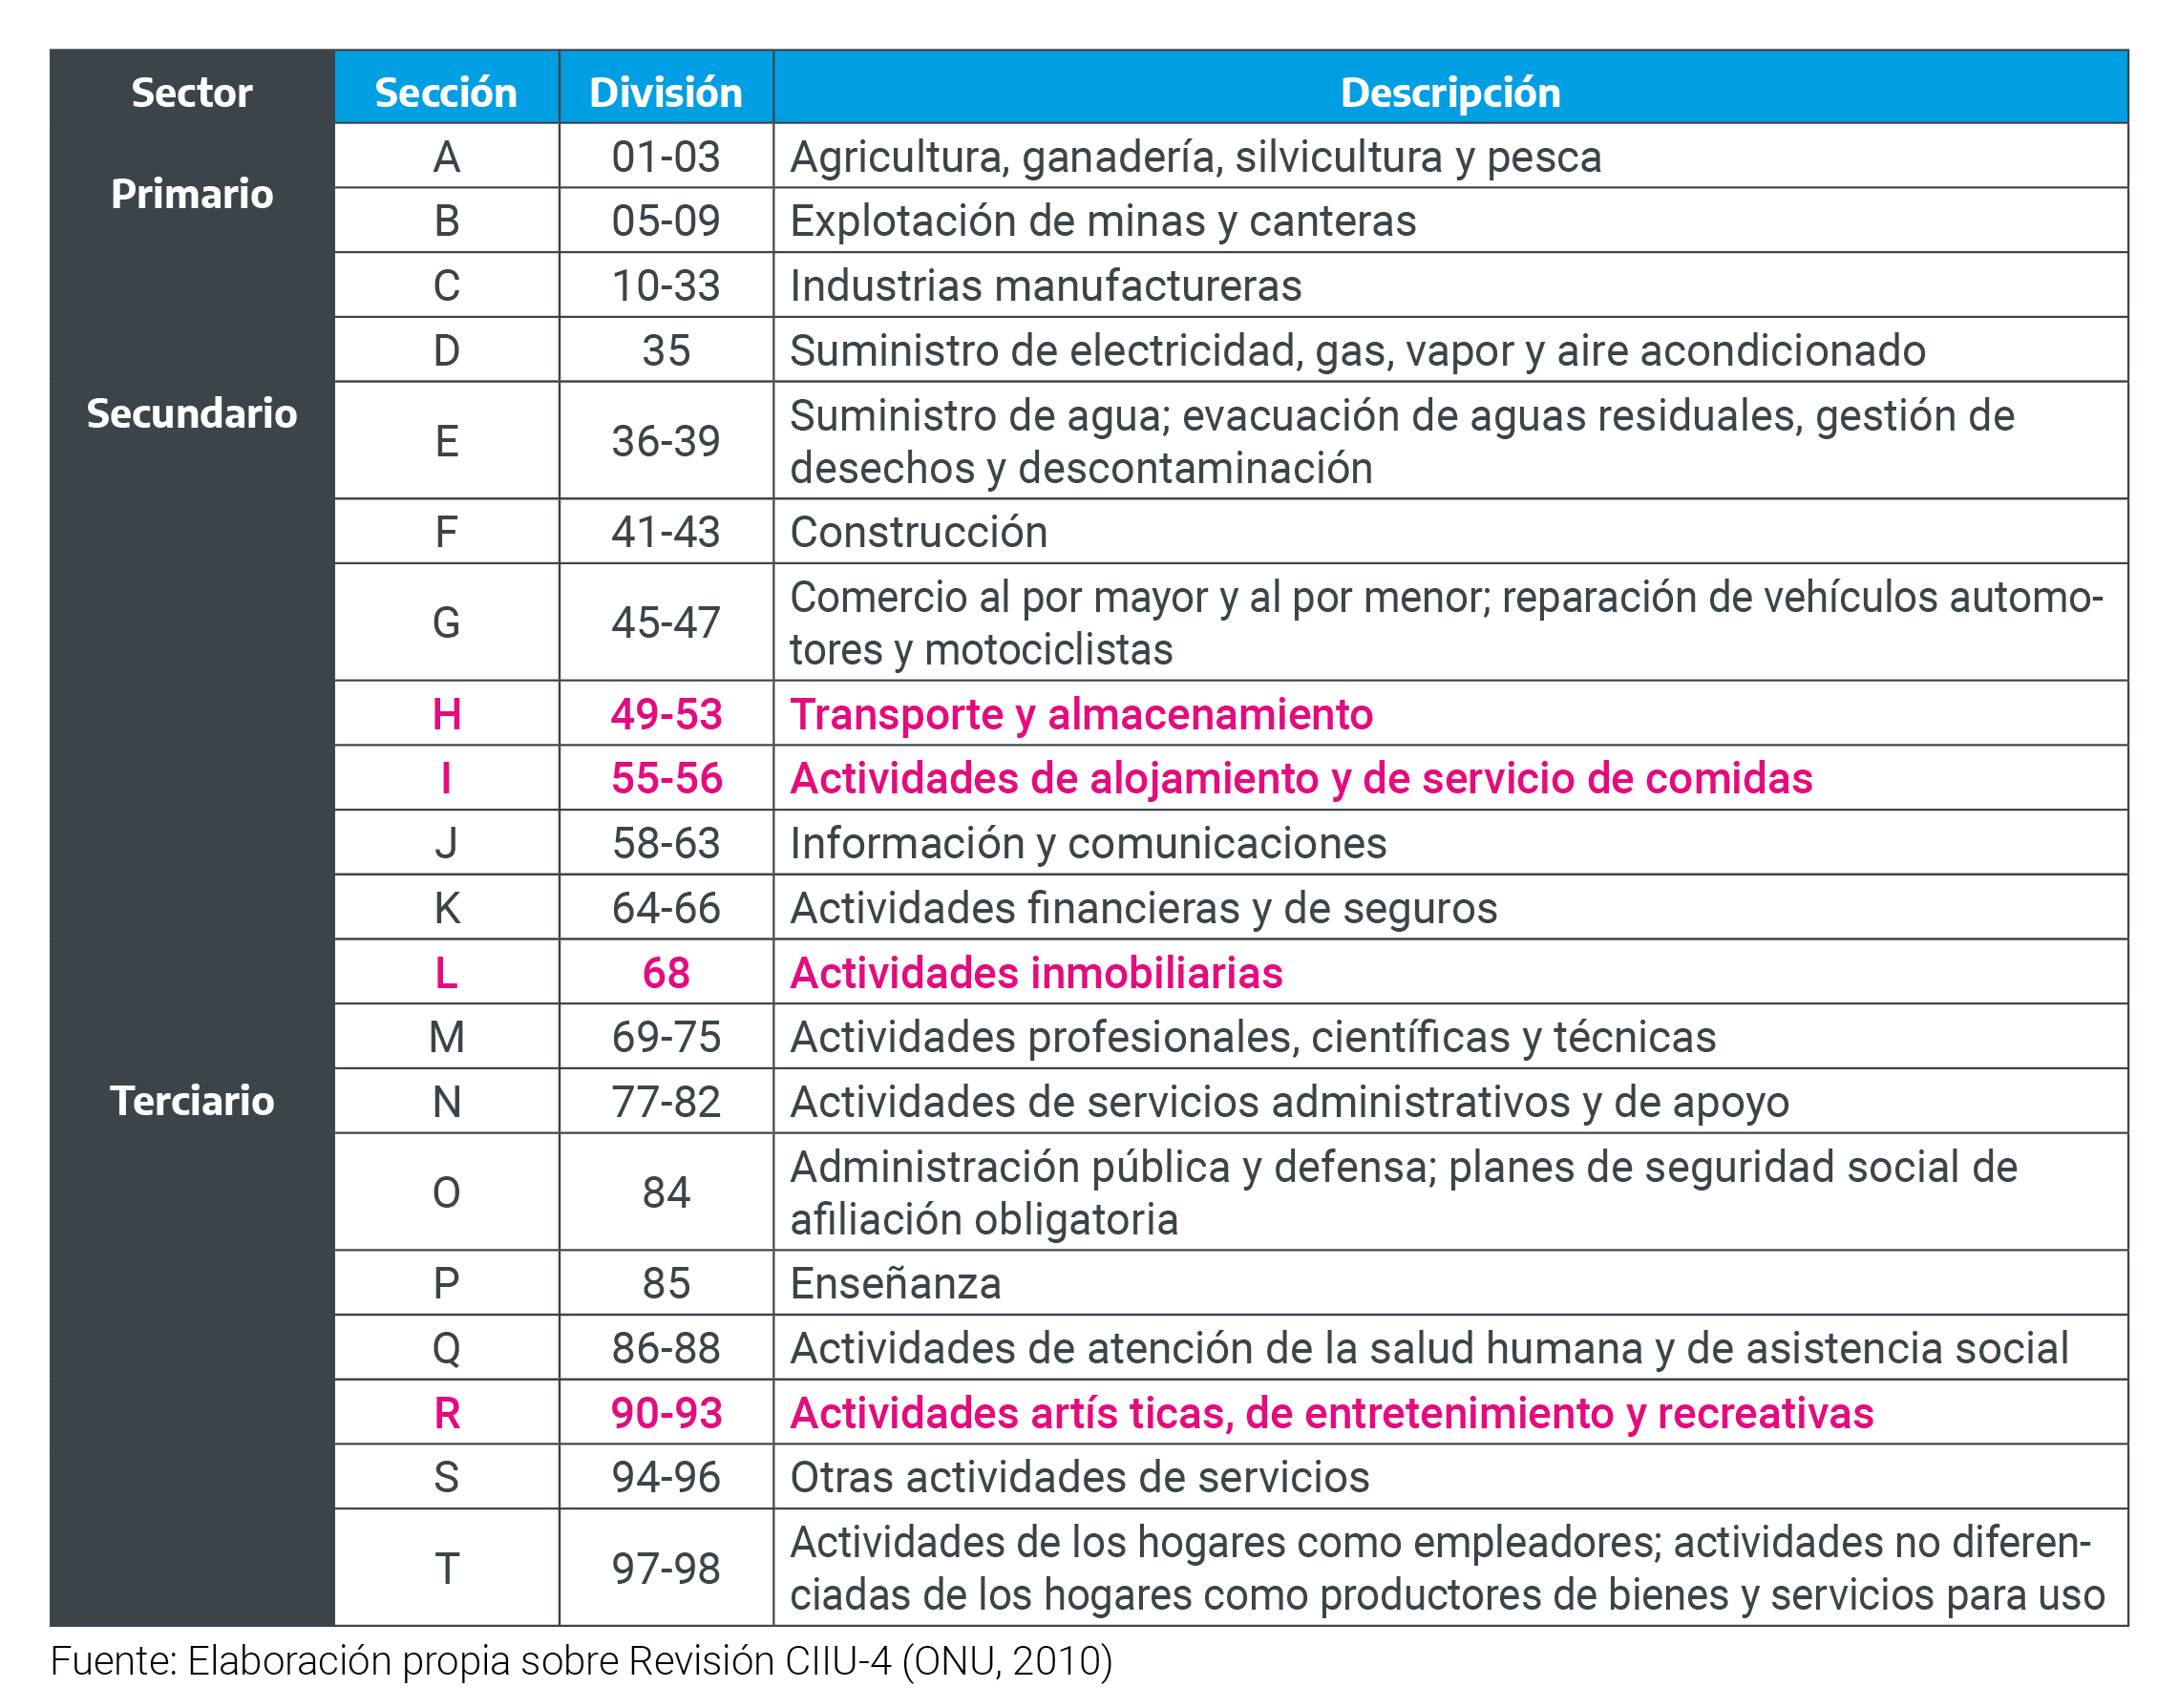
\includegraphics[width=1\linewidth]{imagenes/figura1.1} 

}

\caption{Ramas de Actividad Económica según el Código Industrial Internacional Uniforme}\label{fig:ciiu}
\end{figure}

La CIIU abarca generalmente todas las actividades productivas, es decir, las actividades económicas comprendidas dentro de la frontera de producción del Sistema de Cuentas Nacionales (SCN). Esas actividades económicas se subdividen en una estructura jerárquica integrada por cuatro niveles de categorías mutuamente excluyentes. Las categorías del nivel superior de la clasificación se denominan secciones, identificadas por un código alfabético que tienen por objeto facilitar el análisis económico. Dichas secciones se subdividen en las actividades productivas de grandes grupos, como ``Agricultura, ganadería, silvicultura y pesca'' (sección A), ``Industrias manufactureras'' (sección C) o ``Información y comunicaciones'' (sección J). La clasificación se estructura a partir de esas secciones en categorías cada vez más detalladas, identificadas por un código numérico, que es de dos dígitos para las divisiones, de tres dígitos para los grupos, y de cuatro dígitos para las clases (el nivel más desagregado). Cada establecimiento de la economía se clasificará en una rama de actividad específica según cuál sea su actividad principal, es decir, aquella que genere el mayor valor agregado.

\hypertarget{ramas-caracteristicas}{%
\subsection{Ramas Características del Turismo}\label{ramas-caracteristicas}}

Como se mencionó anteriormente la CIIU está construida sobre un marco conceptual basado en la oferta en el cual se agrupan las unidades de producción en ramas detalladas, priorizando similitudes de su actividad económica, teniendo en cuenta los insumos, los procesos y la tecnología de producción, las características de los productos y los usos a los que se destinan.

Para avanzar es importante definir algunos conceptos en cuanto a la clasificación de la oferta en característica del turismo o no.

Es posible identificar tres agrupaciones por el lado de la oferta que pueden clasificarse como características del turismo: industrias, actividades y productos. La vinculación entre estas tres es la siguiente: Las industrias características del turismo son aquellas cuya actividad principal es característica del turismo. Las actividades características del turismo son aquellas que producen principalmente productos característicos del turismo.

Según el párrafo 5.10 de las Recomendaciones Internacionales para estadísticas de turismo:

\begin{quote}
\emph{"Los productos característicos del turismo son aquellos que cumplen uno o ambos de los siguientes criterios:}

\emph{a. El gasto turístico en el producto debería representar una parte importante del gasto total turístico (condición de la proporción que corresponde al gasto/demanda)}

\emph{b. El gasto turístico en el producto debería representar una parte importante de la oferta del producto en la economía (condición de la proporción que corresponde a la oferta). Este criterio supone que la oferta de un producto característico del turismo se reduciría considerablemente si no hubiera visitantes.}"(\protect\hyperlink{ref-riet2008}{Organización Mundial del Turismo, 2010})
\end{quote}

En adelante, el foco estará puesto en las industrias características del turismo ya que son la base del análisis de la contribución económica del turismo desde la perspectiva de la oferta. En conclusión, el manual de \protect\hyperlink{ref-cstrmc2008}{Oranización Mundial de Tursimo y Organización de Cooperación y Desarrollo Económico} (\protect\hyperlink{ref-cstrmc2008}{2008}) propone la consideración de 10 ramas (industrias) turísticas para la comparación internacional. Adicionalmente, se incorporan 2 líneas de industrias que pueden ser adicionadas por cada región si lo creyera pertinente, según el conocimiento de cómo se desarrolla el turismo dentro de sus límites geográficos. A continuación se presentan estas ramas con el detalle de cada código CIIU (Rev.4 y Rev 3.1) asociado:

\begin{figure}

{\centering 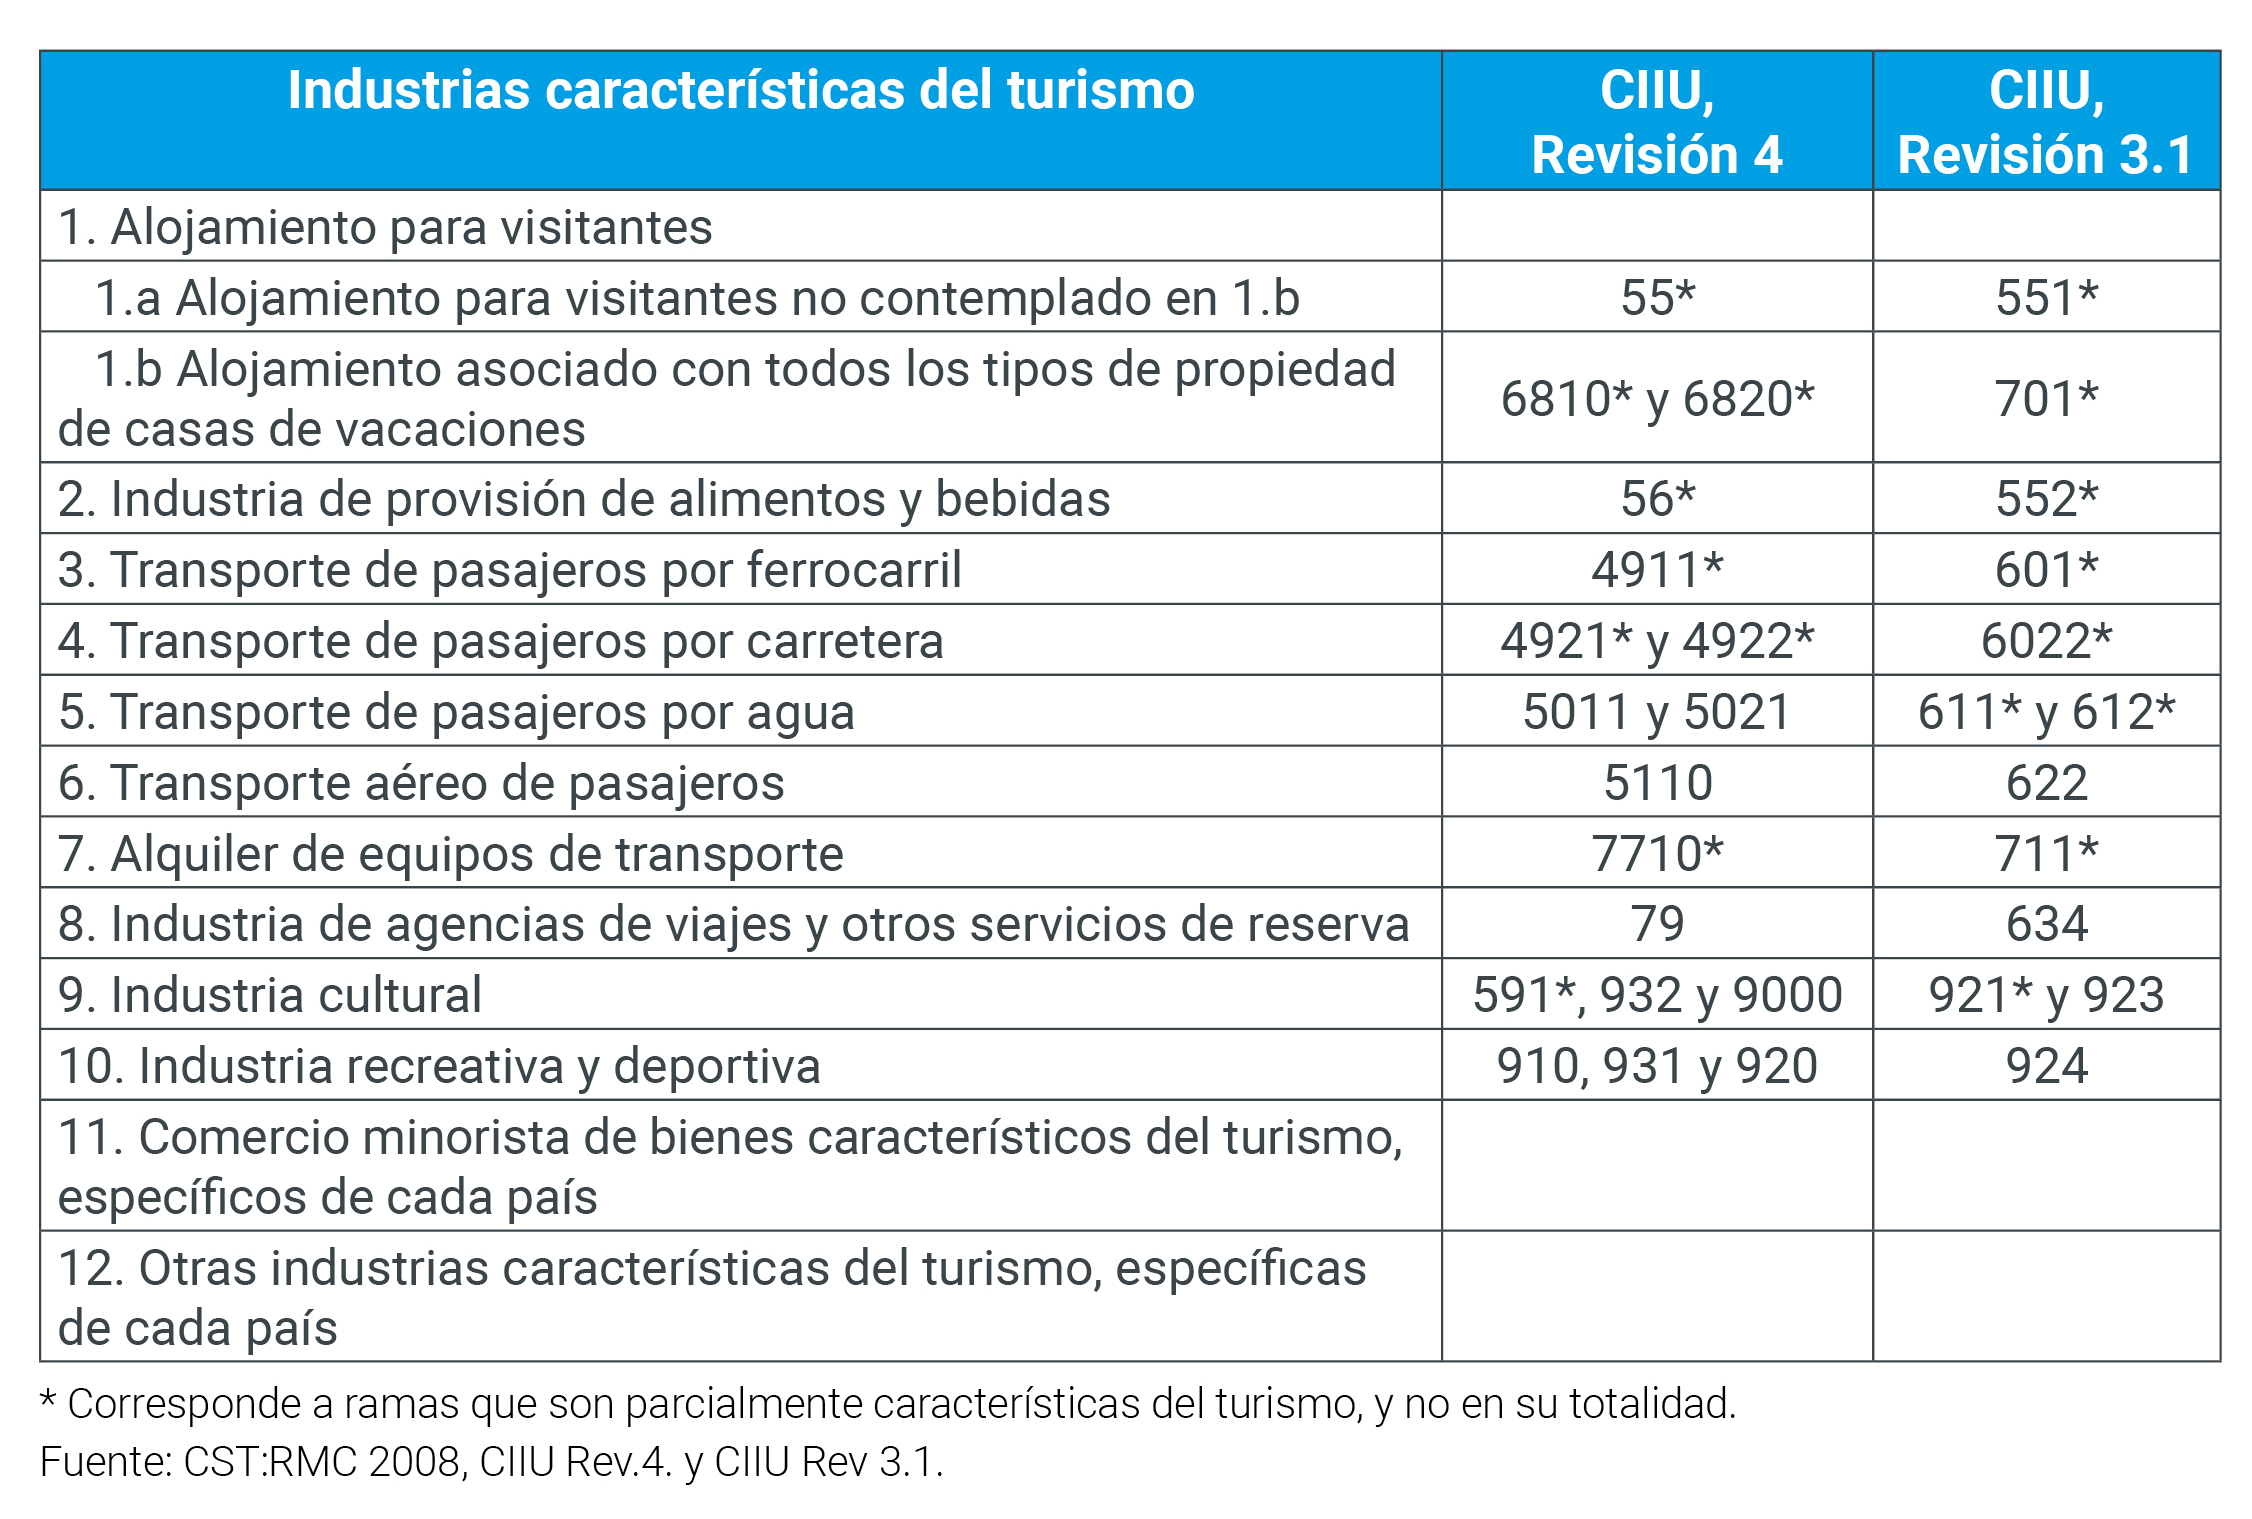
\includegraphics[width=1\linewidth]{imagenes/figura1.2} 

}

\caption{Industrias turísticas y sus códigos CIIU Rev. 4.}\label{fig:ciiu2}
\end{figure}

Se debe tener en cuenta que dichas RCT se consideran como una propuesta, sujeta a que la composición del consumo turístico difiere según la región geográfica. No obstante, es prioritario seguir la agrupación según los códigos CIIU con el fin de mantener la comparabilidad a nivel internacional.

\hypertarget{alcance}{%
\subsection{Alcance}\label{alcance}}

Como se mencionó en el apartado anterior, las industrias turísticas son aquellas cuya actividad principal es característica del turismo. La producción que ellas realicen será el centro de la perspectiva de la oferta para la medición de la contribución económica del turismo. Este enfoque tiene ciertos límites a su alcance que son importantes de explicitar.

\textbf{Destinatario final de la producción}

La perspectiva de la oferta realiza una medición de la contribución del turismo desde el lado de la producción de las industrias turísticas, sin tener en consideración quién consume dicha producción, ni si el mismo es visitante o no. Por lo tanto, dentro de esta perspectiva está incluida la producción que las industrias turísticas realizan pero que no es consumida por visitantes, sino por residentes. En actividades como alojamiento esto no resulta demasiado importante, ya que la mayor parte de la producción de servicios de alojamiento es consumida por visitantes, pero en la actividad de bares y restaurantes o en los servicios de esparcimiento, etc., resulta evidente la importancia de la participación de los residentes en el consumo total.

La situación inversa se presenta en el caso de los consumos de bienes o servicios que los visitantes podrían hacer de industrias no clasificadas como características del turismo. Estos consumos no estarán incluidos en la estimación de la contribución económica del turismo desde la perspectiva de la oferta. Este es el caso del comercio minorista, por ejemplo. Este no es catalogado como una rama característica del turismo aunque los visitantes realizan cuantiosos consumos en esta rama (vestimenta, souvenirs, alimentos y bebidas sin preparación, etc).

\textbf{Establecimientos y actividad principal}

Cada industria turística estará compuesta por todos aquellos establecimientos cuya actividad principal es una actividad característica del turismo. Por lo tanto, si un establecimiento realiza actividades turísticas solo de manera secundaria, no estará incluido dentro de la industria turística caracterizada por esa actividad, por lo tanto, quedará fuera del cálculo de impacto económico del turismo. Un ejemplo de esta situación podría ser: un viñedo obtiene el mayor valor agregado de su actividad de cultivo de vides (actividad principal), pero, a su vez, podría tener alguna casa de huéspedes que ofrezca a visitantes para hospedarse (actividad secundaria). La oferta de esta actividad secundaria de alojamiento turístico no estará incluida en la producción de las industrias turísticas, simplemente porque el establecimiento estará clasificado en la industria asociada a la agricultura, y la misma no es característica del turismo.

Contrariamente, la producción de las industrias turísticas sí incluirá la producción de actividades que los establecimientos turísticos presten de manera secundaria y que no estén vinculadas al turismo. Un ejemplo de este caso podría ser: una agencia de viajes obtiene su mayor valor agregado a partir de la comercialización de paquetes y servicios turísticos en general (actividad principal), pero adicionalmente presta un servicio de concesión de créditos para la financiación de los viajes turísticos, por el cual cobra un interés (actividad secundaria).

En conclusión, es importante notar que la perspectiva de la oferta consiste en un recorte de la producción de una región, siguiendo las recomendaciones internacionales para realizarlo, pero no incorpora en el análisis la demanda efectivamente realizada por visitantes, por lo que no provee una medida de la producción que exclusivamente se generó para atender a los visitantes\footnote{Como se mencionó previamente, el objetivo de este trabajo es profundizar sobre la perspectiva de la oferta para la medición del impacto económico del turismo en una región. Esto implica discriminar con la mayor precisión posible las ramas características, lo cual supone lo ``máximo'' esperable desde el enfoque de la oferta o ramas características.}.

\hypertarget{nivel-de-desagregacion-de-las-ramas}{%
\subsection{Nivel de desagregación de las ramas}\label{nivel-de-desagregacion-de-las-ramas}}

De acuerdo a la descripción realizada sobre el formato de la CIIU, es importante notar que cuanto menor sea el nivel de apertura de la información por rama menor será la precisión de los resultados obtenidos. Por ejemplo, si una determinada fuente brinda los datos globales de Servicios de Transporte Terrestre, la estimación incluirá componentes no relacionados con el turismo (transporte de Carga, por ejemplo), lo cual implica una sobreestimación de la producción de las ramas características del sector.

En contrapartida, cuando la información se presenta en un nivel de detalle mayor permite discriminar mejor qué es y qué no es característico del sector bajo estudio. Por ejemplo, si el transporte terrestre permite distinguir el transporte urbano de pasajeros, del transporte interurbano de pasajeros y del transporte de cargas, resulta evidente que el único que debe ser seleccionado como actividad característica del turismo es el transporte interurbano de pasajeros.

\hypertarget{medicion-de-la-oferta}{%
\section{Medición de la oferta}\label{medicion-de-la-oferta}}

Para una correcta medición del impacto económico del turismo desde la perspectiva de la oferta es fundamental contar con estadísticas robustas sobre la producción de las industrias turísticas. En este apartado se buscará realizar algunas recomendaciones para lograr este objetivo.

\hypertarget{recomendaciones-generales}{%
\subsection{Recomendaciones generales}\label{recomendaciones-generales}}

En primer lugar, se deberá contar con encuestas a las industrias, o bien registros administrativos, que permitan una estimación fiable de la producción en un período determinado. Por lo general, las encuestas anuales a los establecimientos facilitan la obtención de información sobre sus actividades, su producción y sus costos intermedios (para poder calcular el valor agregado de cada uno).

En segundo lugar, como se mencionó en el apartado \ref{nivel-de-desagregacion-de-las-ramas}, la posibilidad de contar con información desagregada de la producción de las RCT es clave porque estará directamente vinculada con la precisión de la estimación de impacto económico. Por lo tanto, se recomienda buscar la generación de estadísticas de oferta que provean una desagregación de las ramas a un nivel de cuatro dígitos de la CIIU, siempre que sea posible.

En tercer lugar, será importante considerar a la informalidad, dependiendo el caso de cada región y de cada actividad a estimar. En este caso, las encuestas a hogares suelen ser la herramienta más útil para calcular la informalidad en la prestación de servicios (particularmente en sectores no tan regulados como el alojamiento, los restaurantes o los servicios de excursiones, por ejemplo).

\hypertarget{agencias-de-viaje-y-operadores-turisticos}{%
\subsection{Agencias de viaje y operadores turísticos}\label{agencias-de-viaje-y-operadores-turisticos}}

Los operadores turísticos combinan dos o más servicios turísticos (transporte, alojamiento, excursiones, etc) y los comercializan a los visitantes de manera directa o a través de agencias de viaje. Las agencias de viaje tratan directamente con los clientes minoristas y proveen el servicio de organización de viajes.

En el caso de este tipo de establecimientos, es importante asegurar que la información recopilada permite discriminar los cobros de las agencias y operadores en sus dos partes fundamentales:

\begin{enumerate}
\def\labelenumi{\arabic{enumi}.}
\item
  el valor de los servicios vendidos (que fueron adquiridos por las agencias u operadores directamente a los prestadores de cada servicio turístico en particular) y
\item
  el margen de comercialización (el pago neto que reciben agencias y operadores por el servicio de organización prestado).
\end{enumerate}

Con el fin de obtener información acerca de los márgenes de comercialización incluidos en los servicios de organización prestados, podrían realizarse encuestas particulares a este tipo de establecimiento que indaguen directamente sobre sus estructuras de costos y los márgenes de ganancia que adicionan al momento de la venta.

\hypertarget{indicadores-macroeconuxf3micos}{%
\section{Indicadores macroeconómicos}\label{indicadores-macroeconuxf3micos}}

Con el objetivo de caracterizar a la oferta turística de una región, se recomienda el cálculo de dos indicadores agregados: el \textbf{Valor Bruto de Producción de las Industrias Turísticas (VBPIT)} y el \textbf{Valor Agregado Bruto de las Industrias Turísticas (VABIT)}.

\hypertarget{valor-bruto-de-produccion}{%
\subsection{Valor Bruto de Producción}\label{valor-bruto-de-produccion}}

En base al Sistema de Cuentas Nacionales (\protect\hyperlink{ref-scn2008}{Fondo Monteario Internacional y Banco Mundial, 2016}) y con el objetivo de caracterizar a la oferta turística de una región se recomienda el cálculo de dos indicadores agregados: el Valor Bruto de Producción de las Industrias Turísticas (VBPIT) y el Valor Agregado Bruto de las Industrias Turísticas (VABIT).

Por lo tanto, el \textbf{VBP de las industrias turísticas (VBPIT)} será el valor de todos los bienes y servicios producidos por las RCT en un territorio y en un período dados.

La valuación del VBPIT se realiza a precios básicos. Los precios básicos son los precios antes de sumar los impuestos sobre los productos y de restar las subvenciones sobre los productos. Es decir, en esta valuación no están incluidos impuestos como IIBB, IVA, impuestos específicos, a los créditos y débitos bancarios, entre otros.

Se recomienda la generación de este indicador para un período de tiempo de un año, ya que permite neutralizar la estacionalidad propia de la actividad turística y reduce el costo de la obtención de información para un período de tiempo menor.

Además del valor monetario del VBPIT, se recomienda calcular su proporción en el total del VBP de la economía bajo estudio.

\hypertarget{valor-agregado-bruto-de-las-industrias-turuxedsticas-vabit}{%
\subsection{Valor Agregado Bruto de las Industrias Turísticas (VABIT)}\label{valor-agregado-bruto-de-las-industrias-turuxedsticas-vabit}}

El VAB es un agregado macroeconómico que mide la producción nueva generada por una industria, país o región, es decir, solo considera el valor que agrega cada una de las industrias a la economía en su totalidad, sin duplicar producciones. Para esto se parte del VBP y a éste se le restan los consumos intermedios (insumos utilizados en el proceso de producción del bien o servicio en cuestión).

El VAB de las industrias turísticas (VABIT) será el valor agregado de todas los establecimientos pertenecientes a industrias consideradas como RCT, sin importar a quiénes estuvo orientada su producción: si a visitantes o a residentes. Como se mencionó en el apartado \ref{alcance}, en este enfoque, el valor agregado bruto no incluye el valor generado por otras industrias no turísticas cuyos productos hayan sido efectivamente adquiridos por visitantes.

Así como el VBPIT, el VABIT se mide a precios básicos.

Así como se sugirió para el VBPIT, se recomienda el cálculo del VABIT anual.

Finalmente, también se recomienda realizar el cálculo de la proporción de VAB generado por las industrias turísticas en el total del VAB de la economía, para tener una noción del peso de las mismas en la economía general.

\hypertarget{antecedentes-en-argentina}{%
\section{Antecedentes en Argentina}\label{antecedentes-en-argentina}}

El Ministerio de Turismo y Deportes de la Nación realizó una estimación de la contribución económica del turismo en la Argentina con base en el año 2004\footnote{El año 2004 es el único año para el cual las cuentas nacionales de Argentina cuentan con Cuadros de Oferta-Utilización (COU). Estos cuadros consisten en un esquema estadístico, elaborado para el año 2004 por la Dirección de Cuentas Nacionales (DNCN) del INDEC, que cuenta con: \textbf{(1)} cuadro de oferta: tiene a las actividades económicas en sus columnas (clasificadas con la CLANAE 2004, compatible con la CIIU Revisión 3) y a los productos (bienes o servicios) producidos por cada una de ellas en sus filas (clasificados con la Clasificación Central de Productos (CPC) de las Naciones Unidas, Revisión 1.1). Presenta entonces la producción de cada actividad económica a nivel de producto, valuados en pesos y a precios básicos; y, \textbf{(2)} cuadro de utilización: tiene a las actividades económicas y a los sectores de demanda final (los hogares, el gobierno, el resto del mundo y las empresas como formadoras de capital bruto) en sus columnas, mientras que en las filas se encuentran los productos (bienes o servicios) utilizados por cada una de las columnas (consumo intermedio, en el caso de las actividades económicas, y consumo final en el caso de los sectores de demanda final). Los valores son presentados en pesos, pero a precios de comprador, es decir, se adicionan impuestos, márgenes de comercio y transporte y se restan las subvenciones. El marco provisto por las COU brinda consistencia en las estimaciones de oferta para cada sector de actividad, es por esto que se utlizó al año 2004 como base para la estimación.} y para los años 2016-2019, con la colaboración de la Dirección Nacional de Cuentas Nacionales (DNCN) del INDEC.

La DNCN proveyó, a pedido del Ministerio de Turismo y Deportes, información de la producción de las actividades económicas a un nivel de desagregación de 4 dígitos de la CIIU Rev.~3, y en algunos casos a 5 o 6 dígitos. De esta manera, fue posible la estimación del impacto económico del turismo desde la perspectiva de la oferta.

Dada la posibilidad de incluir bienes y/o servicios característicos específicos de cada país, para la CST-A se determinó que se considerarían como característicos del turismo a los servicios de expendio minorista de combustibles para automotores (estaciones de servicio). Por ende, su actividad relacionada, venta al por menor de combustible para automotores, también se consideró como característica de turismo.

Las recomendaciones de \protect\hyperlink{ref-riet2008}{Organización Mundial del Turismo} (\protect\hyperlink{ref-riet2008}{2010}) mencionan que \emph{``El combustible para los vehículos de motor (o para embarcaciones en los países insulares) podría representar asimismo un gasto importante en bienes en los países''}. A su vez, se verificó que el gasto en combustibles representó un 10\% del gasto turístico interno que se calculó para la CST-A en el año 2004 para los turistas y un 30\% para los excursionistas.

De esta manera, la apertura de actividades características del turismo para la CST-A quedó determinada de la siguiente manera:

\begin{figure}

{\centering 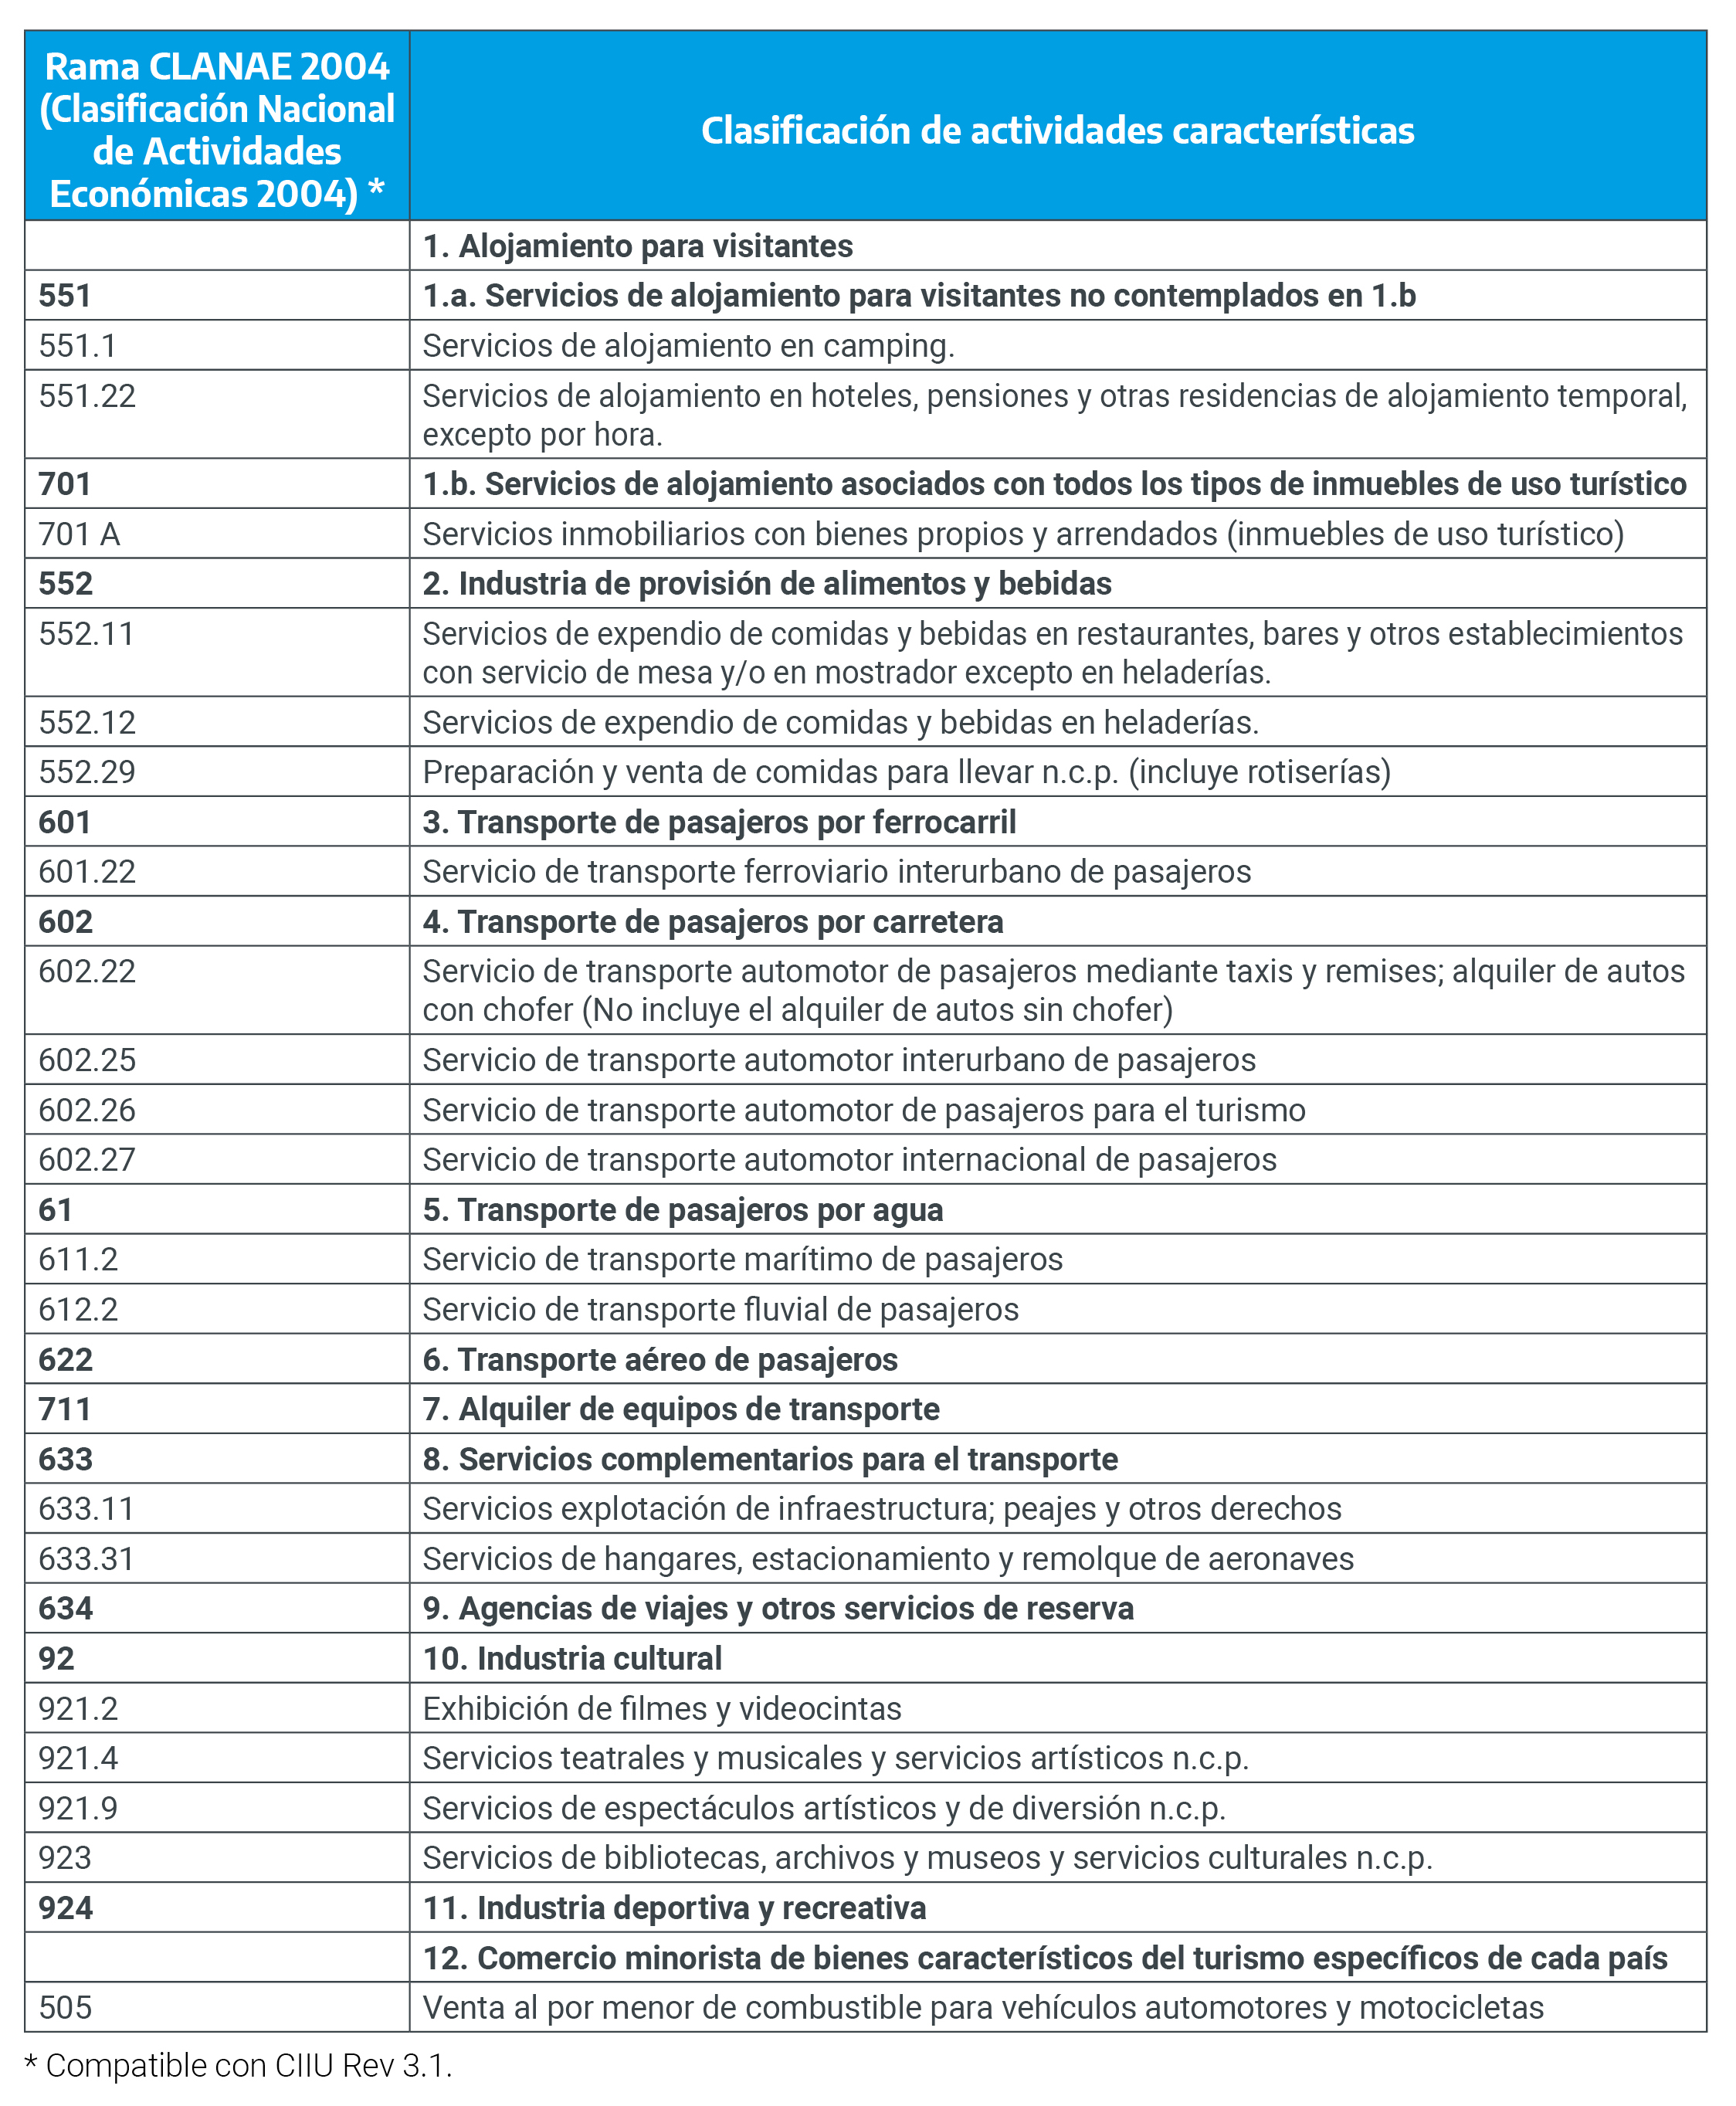
\includegraphics[width=1\linewidth]{imagenes/figrua1.3} 

}

\caption{Actividades Características del Turismo en la CST-A}\label{fig:activcst}
\end{figure}

Por su lado, la producción y el valor agregado de cada industria turística quedó conformado de la siguiente manera:

\emph{En millones de pesos corrientes. A precios básicos.}

\begin{figure}

{\centering 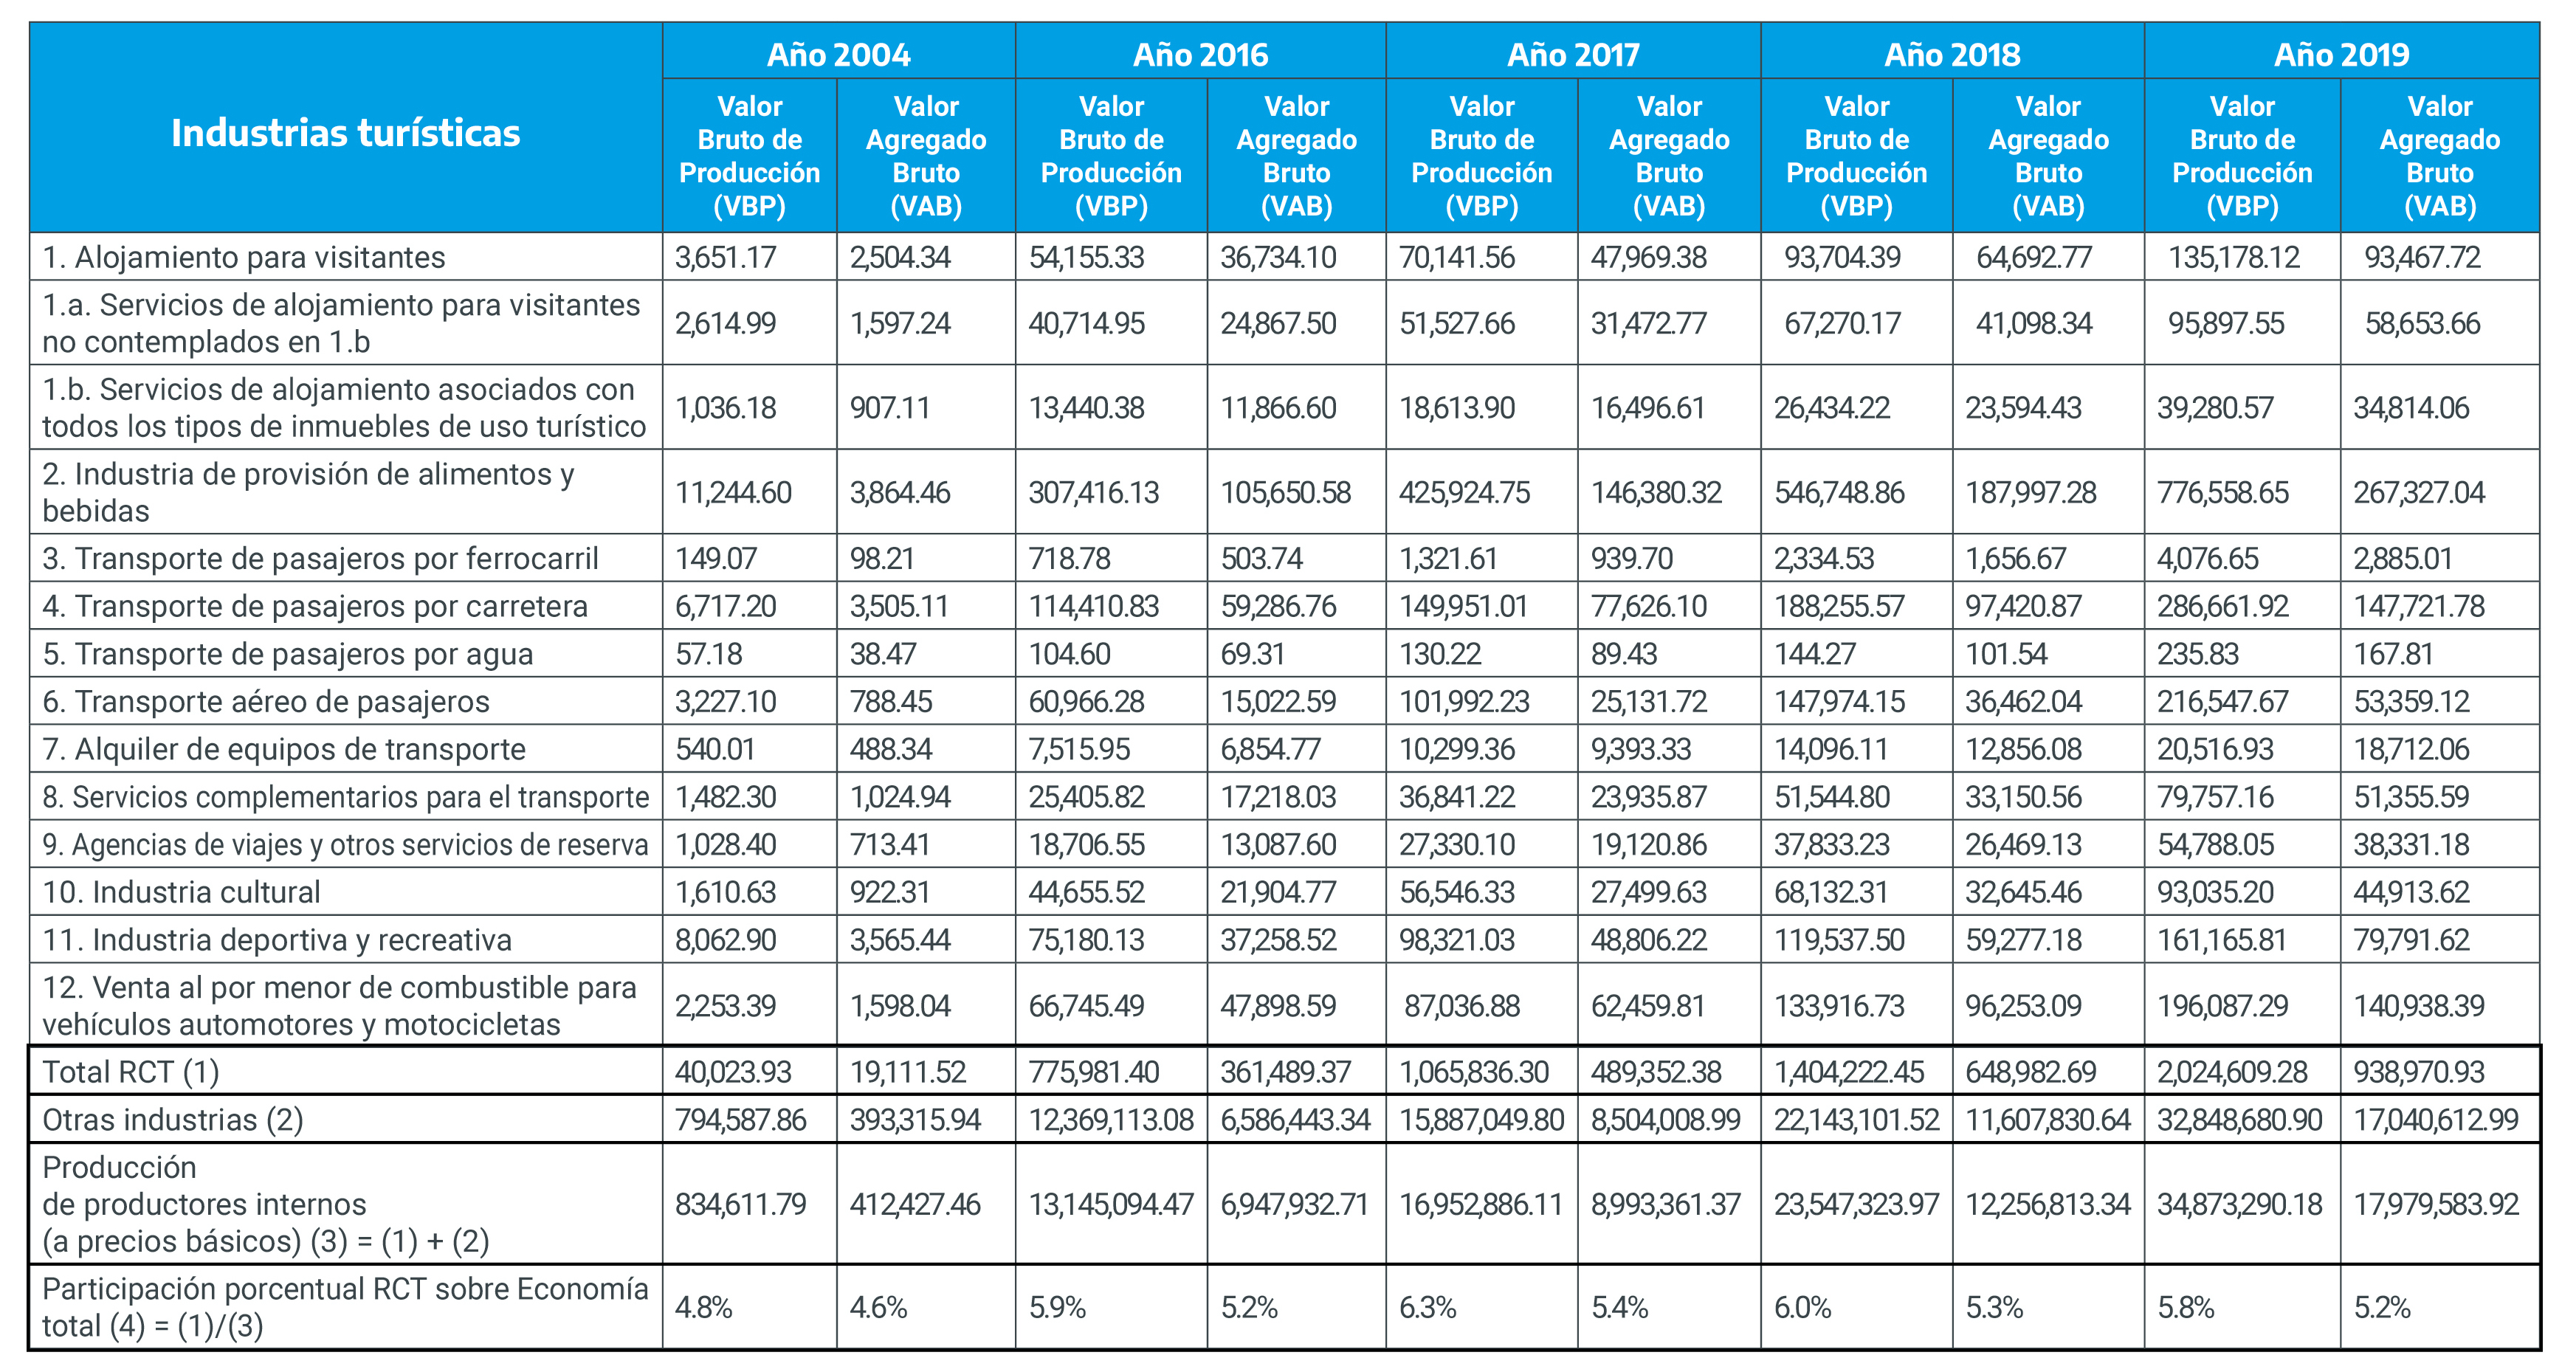
\includegraphics[width=1\linewidth]{imagenes/figura1.4} 

}

\caption{Cuentas de producción de las RCT, Argentina, 2004, 2016-2019}\label{fig:cst}
\end{figure}

Se puede observar que, en el año 2004 y para el total de la Argentina, el VBPIT fue de \$40.023,93 millones, mientras que el VABIT fue de \$19.111,52 millones. En términos relativos el VBPIT fue un 4,8\% del VBP del total de la economía, mientras que el VABIT representó un 4,6\% del VAB total. Hacia los años de la serie 2016-2019 se observa un crecimiento de la producción y valor agregado de las industrias turísticas, dado que en alcanzaron valores más cercanos al 6\% y 5\%, respectivamente.

\hypertarget{medicion-empleo}{%
\chapter{\texorpdfstring{\textbf{La medición del empleo en turismo}}{La medición del empleo en turismo}}\label{medicion-empleo}}

Este capítulo propone un recorrido por los principales conceptos sobre la economía laboral, las metodologías de medición del empleo en el sector turístico (según las recomendaciones de la OMT) y su aplicación tanto en Argentina como en el resto del mundo.

El mercado laboral es definido como el mercado en donde confluyen la demanda y la oferta de trabajo. Los componentes del mercado son expresados en cantidades (puestos de trabajo y personas ocupadas) y precios (salarios) que generalmente se asocian al bienestar de la economía.

La demanda en el mercado de trabajo es efectuada por las empresas para poder desempeñar su actividad económica. La cantidad de trabajadores a emplear dependerá de la cantidad de puestos de trabajo que se requiera ocupar para la actividad en cuestión.

En tanto que la oferta de trabajo es efectuada por las personas a partir de ofrecer sus servicios a las empresas, o trabajar en forma independiente, a cambio de una retribución.

La figura \ref{fig:empleooit} representa una perspectiva esquemática del mercado de trabajo con sus componentes (elementos estructurales) y relaciones. Muestra que las ``personas'' representan el lado de la oferta en el mercado de trabajo, mientras que los ``puestos'' el lado de la demanda. Los casilleros cuadrados en las primeras dos filas incluyen a los empleadores y a los hogares, además de los puestos y las personas. Los ``puestos'' y las ``personas'' se vinculan a través de los empleos.

\begin{quote}
Para mayor información consulte el documento de la \protect\hyperlink{ref-oitconferencia14}{Oficina Internacional del Trabajo} (\protect\hyperlink{ref-oitconferencia14}{2014}).
\end{quote}

En la tercera fila aparecen más casilleros que muestran las subcategorías de puestos y personas ocupadas. El sistema de contabilidad del trabajo requiere que se establezcan estimaciones para todos sus componentes y las relaciones de éstos.

Como se explicará en las secciones siguientes, el empleo en turismo no puede ser observado en forma directa, al menos aquel que se refiere al empleo estrictamente relacionado con los bienes y servicios adquiridos por los visitantes, sin importar si la industria que los produjo es turística o no, por lo tanto, este documento analiza el enfoque de oferta (o ramas características del turismo\footnote{Se utilizarán indistintamente los términos ``Industria'' o ``Rama''})

\begin{figure}

{\centering 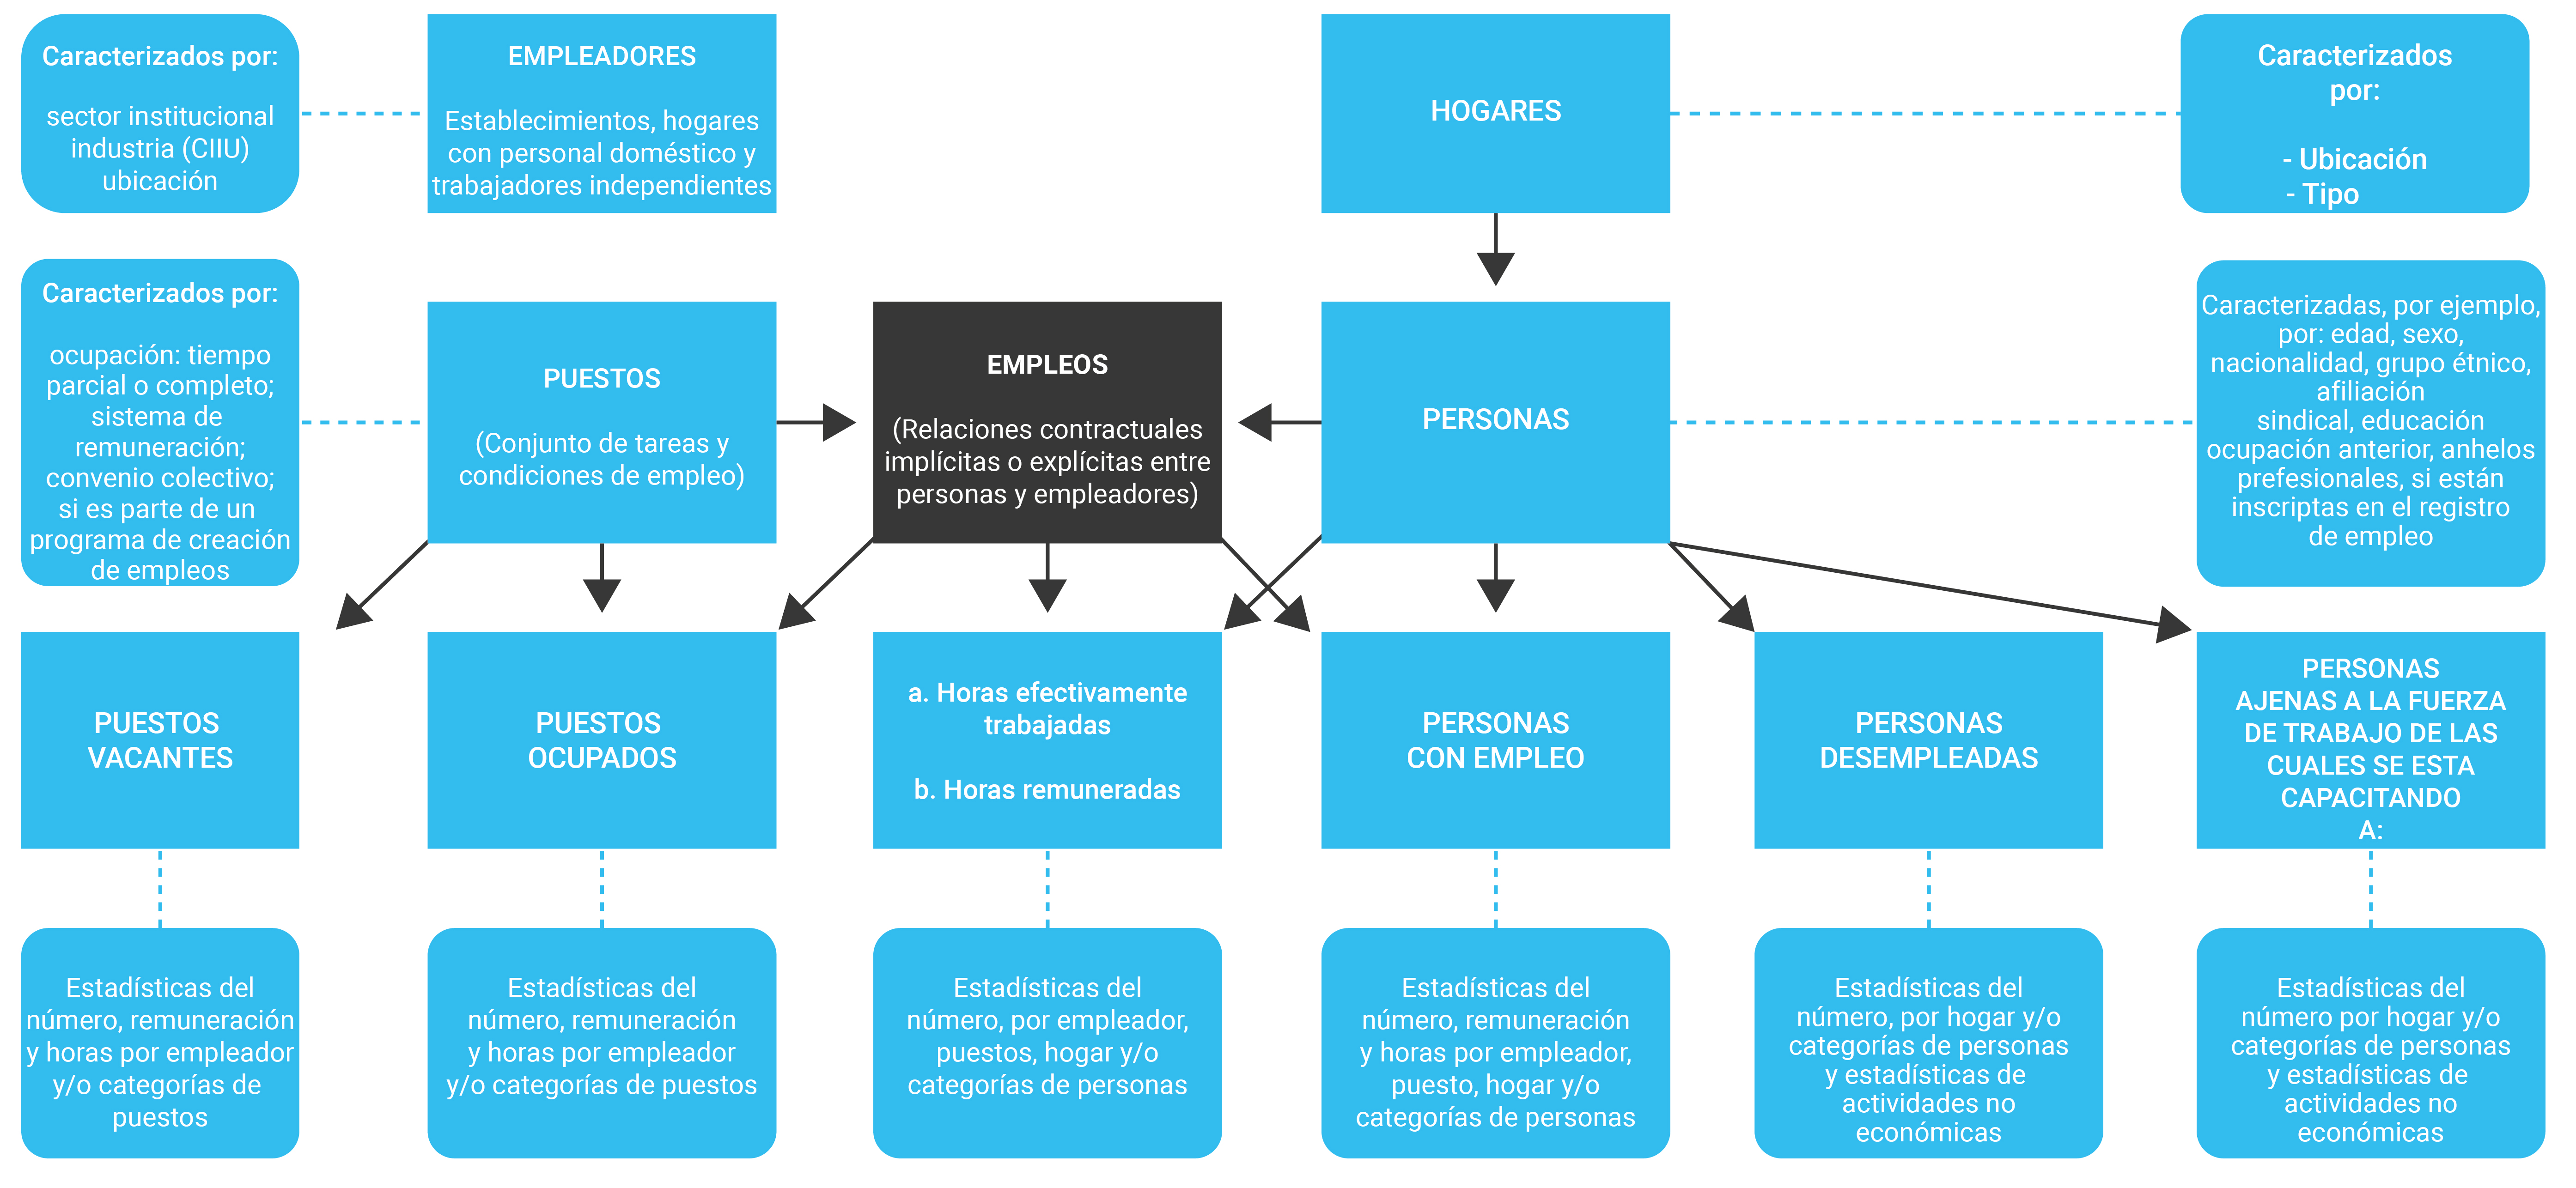
\includegraphics[width=1\linewidth]{imagenes/figura2.1} 

}

\caption{Marco conceptual del Mercado de Trabajo}\label{fig:empleooit}
\end{figure}

\hypertarget{definiciones-generales-sobre-mediciuxf3n-del-empleo}{%
\section{Definiciones generales sobre medición del empleo}\label{definiciones-generales-sobre-mediciuxf3n-del-empleo}}

Es importante conocer a qué se refieren las estadísticas laborales cuando miden trabajo y empleo. Partiendo de la definición de la \href{https://www.ilo.org/global/lang--es/index.htm}{OIT}, el \textbf{trabajo}\footnote{En la actualidad, siguiendo las recomendaciones de la OIT, el concepto trabajo ha sido ampliado a ``Trabajo Decente''. Dicho concepto reconoce que el trabajo promueve la dignidad personal, el crecimiento económico, la estabilidad familiar, la paz en la comunidad, la democracia, la productividad y el desarrollo de las empresas.} corresponde al conjunto de actividades humanas, remuneradas o no, que producen bienes o servicios en una economía, o que satisfacen las necesidades de una comunidad o proveen los medios de sustento necesarios para los individuos. En este contexto, el \textbf{empleo} es definido como el trabajo efectuado a cambio de una remuneración que puede ser denominado salario, sueldo, comisión, propina, pago a destajo o pago en especie sin importar la categoría de empleo (patrón, asalariado, cuentapropista, etc.).

Por otra parte, la OIT categoriza un empleo según el tipo de contrato de trabajo explícito o implícito del titular con otras personas u organizaciones. A partir del año 1993 se creó la Clasificación Internacional de la Situación en el Empleo (CISE, 1993)\footnote{\href{http://www.ilo.org/public/spanish/bureau/stat/download/res/icse.pdf}{Resolución CISE, 1993}} que sirve para agrupar las distintas modalidades vigentes y para comprender su alcance según el sector que se pretenda estudiar. El criterio básico utilizado para definir cada grupo de categoría o clasificación ocupacional está basado en el tipo de \textbf{riesgo económico}, un elemento del cual depende exclusivamente la solidez del vínculo entre la persona y el empleo, y el tipo de responsabilidad que tiene el trabajador sobre el establecimiento.

Las personas con \textbf{\emph{empleos independientes}} pueden dividirse en dos grupos, aquellas que tienen trabajadores asalariados a cargo se clasifican como \textbf{\emph{``empleadores''}} o \textbf{\emph{``patrones''}}, mientras que aquellas que no los tienen se clasifican como \textbf{\emph{``trabajadores por cuenta propia''}}. El término empleo independiente alcanza aquel tipo de trabajo donde la remuneración depende directamente de los beneficios (o del potencial para realizar beneficios) derivados de los bienes o servicios producidos (el consumo propio forma parte de los beneficios). El titular toma las decisiones operacionales que afectan a la empresa, o delega tales decisiones, pero mantiene la responsabilidad por el bienestar de la empresa.

Por otro lado, los trabajadores con un empleo asalariado son clasificados dentro de la categoría \textbf{\emph{``empleo en relación de dependencia''}}, situación que refiere a aquel trabajador que recibe una remuneración básica que no depende directamente de los ingresos de la unidad para la que trabaja.

Cabe aclarar que todas las categorías mencionadas anteriormente pueden identificarse tanto en el marco de la economía formal como de la economía informal. El término \textbf{\emph{``economía informal''}} hace referencia al:

\begin{quote}
\emph{``conjunto de actividades económicas desarrolladas por los trabajadores y las unidades económicas que, tanto en la legislación como en la práctica, están insuficientemente contempladas por sistemas formales o no lo están en absoluto. Las actividades de esas personas o empresas pueden no estar alcanzadas por la ley, es decir, se desempeñan al margen de ella; o bien no están contempladas en la práctica, es decir que, si bien estas personas operan dentro del ámbito de la ley, ésta no se aplica o no se cumple.''}(\protect\hyperlink{ref-oitconferencia14}{Oficina Internacional del Trabajo, 2014})
\end{quote}

Además, existen grandes diferencias entre los trabajadores de la economía informal en cuanto a ingresos (nivel, regularidad, estacionalidad), situación en el empleo (asalariados, empleadores, trabajadores por cuenta propia, trabajadores ocasionales, trabajadores domésticos), sector (comercio, agricultura, industria), tipo de empresas y tamaño de las mismas, ubicación geográfica (medio urbano o rural), protección social (contribuciones a la seguridad social), y protección del empleo (tipo y duración del contrato, derecho a vacaciones anuales).

Por lo tanto, en un sistema económico los trabajadores pueden desempeñarse bajo una modalidad de Empleo Formal o Empleo Informal. La distinción entre uno u otro está dada por el cumplimiento de la legislación laboral en relación con las personas involucradas en la unidad productiva o en su propio emprendimiento económico cumpliendo con alguna de las normas que regulan sus actividades económicas y las obligaciones previsionales.

En síntesis, se considera que los trabajadores se encuentran en la modalidad de un \textbf{\emph{Empleo Informal}}\footnote{Según la OIT, las razones pueden ser las siguientes: la no declaración de los empleos o de los asalariados; empleos ocasionales o empleos de limitada o corta duración; empleos con un horario o un salario inferior a un límite especificado (por ejemplo para cotizar a la seguridad social); el empleador es una empresa no constituida en sociedad o una persona miembro de un hogar; el lugar de trabajo del asalariado se encuentra fuera de los locales de la empresa del empleador (por ejemplo, los trabajadores fuera del establecimiento y sin contratos de trabajo); empleos a los cuales el reglamento laboral no se aplica, no se hace cumplir o no se hace respetar por otro motivo.} si su relación de trabajo, de derecho o de hecho, no está sujeta a la legislación laboral nacional, la protección social o a determinadas prestaciones relacionadas con el empleo (cobertura jubilatoria con descuento, cobertura jubilatoria con aporte voluntario, preaviso al despido, indemnización por despido, vacaciones anuales pagadas o licencia pagada por enfermedad, etc.).

Por lo tanto, las principales definiciones a tener en cuenta son (\protect\hyperlink{ref-oit2004}{Organización Internacional del Trabajo, 2004}):

\begin{itemize}
\tightlist
\item
  \textbf{Persona ocupada\footnote{En Argentina se considera como persona ocupada a todos los individuos que tengan cierta edad específica (10 años o más) y que durante un período de referencia (una semana) hayan trabajado al menos una hora. Incluye: a) las personas que durante el período de referencia realizaron algún trabajo de al menos una hora, sin importar si recibieron pago (en dinero o en especie) o no por dicha actividad; b) las personas que tienen una ocupación, pero que no están trabajando temporalmente durante el período de referencia y mantienen un vínculo formal con su empleo. Integran este grupo los ocupados que no trabajaron en la semana, por vacaciones, licencia por enfermedad u otros tipos de licencias, suspendidos con pago y ausentes por otras causas laborales (mal tiempo, averías mecánicas, escasez de materias primas, etc.) con límite de tiempo de retorno. Se incluyen también dentro de esta categoría a las personas que tienen un negocio o empresa y no trabajaron por causas circunstanciales durante el período de referencia.}:} es un individuo físico que realiza ciertas tareas laborales, pudiendo ocupar uno o más puestos de trabajo;
\item
  \textbf{Puesto ocupado:} corresponde a una persona empleada para realizar un conjunto de tareas en una empresa o negocio;
\item
  \textbf{Empleador o Patrón:} es aquel que, trabajando por su cuenta o con uno o más socios, ha contratado a una o a varias personas para que trabajen en su empresa como ``asalariados'' a lo largo de un período continuo que incluye el período de referencia. Los titulares pueden tomar las decisiones operacionales que afectan a la empresa, o bien delegarlas, pero mantienen la responsabilidad por el bienestar de la empresa;
\item
  \textbf{Trabajador por cuenta propia:} es aquel trabajador que, trabajando por su cuenta o con uno o más socios, no ha contratado a ningún ``asalariado'' de manera continua durante el período de referencia. Cabe notar que durante el período de referencia los miembros de este grupo pueden haber contratado ``asalariados'', siempre y cuando lo hagan de manera esporádica;
\item
  \textbf{Asalariado:} es aquel trabajador que tiene un empleo en relación de dependencia y que posee, por lo tanto, un contrato de trabajo implícito o explícito (oral o escrito) con el mismo empleador de manera continua. Los empleados asalariados son los trabajadores que reciben una remuneración básica, la cual no depende directamente de los ingresos de la unidad para la que trabaja. Además, la organización empleadora es responsable por el pago de las cargas fiscales y de las contribuciones de la seguridad social del empleado (a partir de las exigencias de la legislación nacional de trabajo).
\end{itemize}

\begin{quote}
\textbf{AGREGAR ALGUNOS CONCEPTOS DE:}
\textbf{EMPLEO VERDE }
\textbf{EMPLEO DECENTE}
\end{quote}

\hypertarget{recomendaciones-internacionales-sobre-el-empleo-en-industrias-turuxedsticas}{%
\section{Recomendaciones Internacionales sobre el empleo en industrias turísticas}\label{recomendaciones-internacionales-sobre-el-empleo-en-industrias-turuxedsticas}}

Las Recomendaciones Internacionales sobre Estadísticas de Turismo (\protect\hyperlink{ref-riet2008}{Organización Mundial del Turismo, 2010}) describen dos formas de medir el empleo relacionado con el turismo. Por un lado, se denomina Empleo Turístico \emph{``al empleo estrictamente relacionado con los bienes y servicios (característicos del turismo, el turismo conexo y otros) adquiridos por los visitantes y producidos por cualquiera de las industrias del turismo y otras industrias''}, mientras que el Empleo en las Industrias Turísticas se refiere al empleo en las actividades características del turismo.

Las RIET 2008 sugieren un marco metodológico para medir el nivel y características del empleo generado por la industria del turismo \emph{desde una perspectiva de la oferta}, a través de la selección de empresas o industrias características del turismo. Es decir, se tiene en cuenta el empleo generado en una selección de ramas de actividad económica características del Turismo.

Además, menciona las particularidades del sector a la hora de estimar el empleo turístico, haciendo referencia a que las actividades características del turismo suelen requerir abundante mano de obra, que, si bien puede asociarse a la producción total de un establecimiento, no puede asignarse a una producción particular \emph{sin la utilización de hipótesis y de procedimientos de modelización}.

Por este motivo, no se puede observar directamente el empleo en turismo, haciendo referencia al empleo estrictamente relacionado con los bienes y servicios (característicos del turismo, conexos al turismo y de otro tipo) adquiridos por los visitantes y producidos por las industrias turísticas u otras industrias.

Dado que el objetivo de este trabajo es explorar las estadísticas del empleo en el sector turístico, el enfoque será puesto en el empleo en las industrias turísticas, es decir, el empleo en el sector, con independencia de que los productos y/o servicios fueran adquiridos por los turistas o no. Del mismo modo, no serán contempladas aquellas ramas de actividad que producen bienes o servicios que los visitantes eventualmente pueden consumir, pero que no constituyen industrias características del sector.

\hypertarget{empleo-en-las-ramas-de-actividad-econuxf3mica}{%
\section{Empleo en las ramas de actividad económica}\label{empleo-en-las-ramas-de-actividad-econuxf3mica}}

Las estimaciones del empleo en el sector turístico se verían resueltas con facilidad si pudieran ser calculadas en base al volumen de los bienes y servicios consumidos únicamente por los turistas. Sin embargo, la asociación de un nivel de empleo a un volumen de bienes y servicios es muy difícil de lograr y de justificar teóricamente. Por esta razón, para identificar el empleo en las industrias turísticas se debe recurrir a la selección de las ramas características, lo cual, además, permite identificar la composición del empleo turístico por categoría ocupacional.

Con este objetivo, se utilizará la CIIU Revisión 4 (\protect\hyperlink{ref-ciiurev4}{Organización de las Naciones Unidas, 2009}) y la correspondiente delimitación de ramas características del turismo, tal como se explicita en la sección \ref{ramas-caracteristicas} del presente documento.

\hypertarget{dificultades-generales-para-la-estimaciuxf3n-del-empleo-en-la-industria-turuxedstica}{%
\section{Dificultades generales para la estimación del empleo en la industria turística}\label{dificultades-generales-para-la-estimaciuxf3n-del-empleo-en-la-industria-turuxedstica}}

Desde los postulados planteados, el análisis de las fuentes que brindan información sobre el mercado de trabajo en Argentina permite adelantar un conjunto de problemas específicos para el abordaje de la medición del empleo en turismo a partir del enfoque de ramas características. La metodología de estimación diseñada procura solucionar, de la \emph{mejor forma posible}, los siguientes problemas:

\begin{itemize}
\tightlist
\item
  \textbf{Identificación de las empresas del sector:} dificultad para definir con exactitud las empresas (y sus trabajadores) dedicadas a ofrecer productos y/o servicios al sector y para extraer aquellos componentes no turísticos a partir del cruce de las distintas fuentes de información, debido a los diferentes niveles de desagregación con que se presenta la información y/o a la utilización de distintos nomencladores de la actividad económica.
\item
  \textbf{Estacionalidad:} las fluctuaciones de la demanda turística introducen variaciones en el volumen del empleo. Esto es especialmente claro en el dominio de la pequeña empresa familiar, en donde la contratación temporal permite cubrir épocas de mayor demanda. Adela Mariscal en su trabajo ``Mercado de Trabajo y turismo en Andalucía'' (\protect\hyperlink{ref-mariscal2005}{Mariscal Galeano, 2005}) señala que donde existen estructuras consolidadas (pymes, cadenas hoteleras, etc.), la estabilidad y la calidad del empleo son mayores, pero que en los casos de micropymes, cooperativas, sociedades anónimas laborales, etc., y donde además puede existir vulnerabilidad económica y territorial, el empleo es altamente estacional. Esta reflexión, sin dudas, aplica también para el caso argentino.
\item
  \textbf{Trabajo informal:} el alto nivel de empleo informal puede implicar la subestimación del impacto del turismo en el empleo. Según el documento ``Empleo y Recursos Humanos en España'' (Sancho, 1998), los principales sectores de la economía informal son la agricultura y los servicios (hoteles y restaurantes, servicios privados de limpieza y trabajo doméstico). Además, existe una alta rotación de los empleos, que es más significativa en el sector hotelería y restaurantes, con tasas superiores al 30\% (Greffe, 1994; OIT, 1997). Los principales afectados son los asalariados de pequeños y medianos establecimientos, los cuentapropistas y los trabajadores familiares no remunerados. Resulta evidente que obtener información robusta sobre este subuniverso es más complejo que hacerlo sobre los establecimientos o empleados formalizados.
\item
  \textbf{Periodicidad:} continuidad en la disponibilidad de los datos, así como antigüedad de las series.
\item
  \textbf{Cobertura:} falta de cobertura de la totalidad del territorio (geográfico o económico) bajo estudio.
\item
  \textbf{Robustez y fiabilidad:} las encuestas por muestreo implican diseños que no permiten realizar estimaciones pequeñas con márgenes de error razonables. Esto implica necesariamente el desarrollo de estrategias que utilicen las estimaciones del modo más agregado posible pero que, a su vez, permita dar cuenta de las aperturas relevantes que se procuran estimar (provincia, sector, categoría ocupacional).
\end{itemize}

** Se puede agregar una sección sobre recomendaciones generales a tener en cuenta para estimar el empleo. Tipo, qué sería bueno que tengan en cuenta al momento de relevar información como para poder obtener información robusta (símil sección 1.2.1 del cap 1)**

\hypertarget{antecedentes-de-la-mediciuxf3n-del-empleo-en-turismo-en-argentina}{%
\section{Antecedentes de la medición del empleo en turismo en Argentina}\label{antecedentes-de-la-mediciuxf3n-del-empleo-en-turismo-en-argentina}}

En Argentina, el Ministerio de Turismo y Deportes de la Nación con la colaboración de la Dirección Nacional de Cuentas Nacionales (DNCN) del INDEC realizó una estimación del volumen de empleo en las ramas de actividad características del turismo con base en el año 2004 y la serie para los años 2016-2019, consistentes con la estimación del nivel de actividad de la industria del turismo.

La DNCN proveyó, a pedido del Ministerio de Turismo y Deportes, información de los puestos de trabajo de las actividades económicas a un nivel de desagregación de 3 dígitos de la CIIU Rev.~3, y para los asalariados privados registrados a 5 dígitos. De esta manera, fue posible la estimación de la contribución del empleo del turismo desde la perspectiva de la oferta.

Para los resultados de las estimaciones realizadas se logró apertura para las ramas agrupadas en las siguientes categorías:

\begin{itemize}
\tightlist
\item
  \textbf{Agencias de viaje:} \emph{agencias de viaje.}
\item
  \textbf{Transporte terrestre:} \emph{ferroviario interurbano; taxis y remises; automotor interurbano; automotor para el turismo.}
\item
  \textbf{Transporte acuático:} \emph{marítimo y fluvial de pasajeros.}
\item
  \textbf{Transporte aéreo:} \emph{aéreo de pasajeros.}
\item
  \textbf{Servicios anexos del transporte:} \emph{peajes.}
\item
  \textbf{Alojamiento:} \emph{camping; hoteles, hosterías y similares; Servicios inmobiliarios realizados por cuenta propia, con bienes propios o arrendado.; Servicios inmobiliarios realizados a cambio de una retribución o por contrato.}
\item
  \textbf{Gastronomía:} \emph{restaurantes y similares; comidas por vendedores ambulantes; rotiserías.}
\item
  \textbf{Otros:} \emph{cines; espectáculos teatrales, musicales y artísticos; artísticos y de diversión NCP; bibliotecas; museos y preservación de lugares y edificios históricos; botánicos, zoológicos y parques nacionales; otros culturales; prácticas deportivas; salones de juegos y entretenimiento NCP}.
\end{itemize}

Los datos de la estimación se presentan desagregados en las siguientes categorías ocupacionales (que surgen, más precisamente, de la combinación entre el nivel de formalidad y de independencia de los trabajadores):

\begin{itemize}
\tightlist
\item
  \textbf{Asalariados Registrados (AR):} obreros o empleados con descuento jubilatorio realizado por el empleador
\item
  \textbf{Asalariados No Registrados (ASNR):} obreros o empleados sin descuento jubilatorio realizado por el empleador
\item
  \textbf{No Asalariados (NOASAL):} patrones, cuentapropistas y trabajadores familiares no remunerados.
\end{itemize}

En cuanto a las fuentes de información, la principal es la Cuenta Generación del Ingreso elaborada por la DNCN, que ofrece el dato (con una periodicidad cuatrimestral) de la cantidad de puestos de trabajo por rama de actividad desagregados en asalariados registrados (ASR), asalariados no registrados (ASNR) y no asalariados (NOASAL). La limitación de ésta es el nivel de desagregación presentado. En segundo lugar, el registro administrativo del Sistema Integrado Previsional Argentino (SIPA) tiene como la principal ventaja su confiabilidad y su cobertura, ofreciendo un registro de todos los trabajadores asalariados mayores de 18 años que se desempeñan en el sector privado cuyos aportes previsionales son realizados por sus empleadores.

Los resultados se presentan en la tabla siguiente:

Existen también otros trabajos realizados en años anteriores que tratan la estimación del empleo en el sector turístico. Uno de ellos es \emph{``El empleo en ramas características del turismo en Argentina''} (\protect\hyperlink{ref-mintur2007}{Ministerio de Turismo y Deportes, 2007}), donde se propone un estudio ``desde el punto de vista de la oferta, es decir estudiando el empleo en las ramas características del turismo'' utilizando la Encuesta Permanente de Hogares (EPH) como fuente de información. Para la definición de las RCT toma como referencia la lista propuesta por la OMT, a fin de mantener la comparabilidad internacional.

Partiendo de dicha clasificación, se estima el volumen de empleo en las RCT en Argentina, dedicando un apartado a describir las características sociodemográficas del empleo en el sector. Sin embargo, cabe señalar que la EPH sólo cubre algo más del 60\% de la población nacional, puesto que se releva en los 31 grandes aglomerados del país. Por otro lado, la desagregación de la información por rama de actividad no permite discriminar, en muchos casos, componentes turísticos y no turísticos dentro de un mismo código de actividad (por ejemplo, ``Transporte terrestre de pasajeros'' incluye tanto el urbano como el interurbano, cuando es este último el único que debería considerarse como turístico).

Para analizar la estacionalidad del sector, utiliza la Encuesta de Ocupación Hotelera (EOH) para estimar las variaciones estacionales de los puestos de trabajo en una rama específica, los hoteles. Cabe indicar que en este caso los resultados obtenidos se refieren a puestos de trabajo, en lugar de personas ocupadas (como corresponde a las estimaciones sobre la EOH).

Por otro lado, la \emph{Cámara Argentina de Turismo utilizó} un procedimiento de cálculo desde una perspectiva de la Demanda para estimar el empleo, como lo explica en su \emph{``Informe económico anual sobre la actividad de viajes y turismo (2008)''}. Utiliza el Método de Coeficientes Fijos (ratios) para estimar el nivel de empleo por rama y categoría, donde se aproxima a la cantidad de empleo generada por la actividad económica de turismo y viajes bajo el supuesto de construcción de coeficientes fijos.

En este sentido, los coeficientes recorren transversalmente las actividades económicas de cuentas nacionales vinculadas de forma directa e indirecta con el sector turismo para estimar su participación en el Producto Interno Bruto (PIB). En particular, a partir de estimaciones de la demanda que realizan los turistas de productos ofrecidos por los distintos sectores económicos se determinan los coeficientes de participación del turismo sobre el valor agregado bruto de cada una de estas actividades. Esto implica que, por ejemplo, al sector hotelero, en el cual el sector turismo tiene una importancia significativa, se le aplique un coeficiente de 100\% y, por el contrario, a la industria manufacturera, que produce tanto para visitantes como no visitantes, se le asigne un coeficiente sustancialmente menor.

Cada uno de estos coeficientes mide el porcentaje del valor agregado de cada actividad económica que pertenece al turismo. No obstante, lo interesante de este ejercicio, es cuestionable su validez empírica por la dificultad de obtener sus coeficientes con cierta confiabilidad a partir de la información disponible al momento de su elaboración.

\hypertarget{fuentes-informacion}{%
\chapter{\texorpdfstring{\textbf{Fuentes de información}}{Fuentes de información}}\label{fuentes-informacion}}

En este capítulo se presentan las fuentes de información disponibles para la medición de la contribución económica, en términos de actividad y empleo, de las Ramas Características del Turismo a nivel provincial, con el fin de analizar la heterogeneidad y limitaciones de cada una.

Es importante destacar que, en la actualidad, algunas fuentes de información que corresponden a operativos puntuales con períodos de realización de varios años no cuentan con información actualizada a los años recientes. Este es el caso de los censos económico y de población. Sin embargo, se espera que en los próximos años se publiquen nuevas ediciones de ambos operativos.

\hypertarget{tipos-de-fuentes}{%
\section{Tipos de fuentes}\label{tipos-de-fuentes}}

Las fuentes de datos disponibles se pueden diferenciar en cinco clases:

\begin{itemize}
\item
  \textbf{Encuestas a hogares}: Permite captar las características sociodemográficas de la población de manera regular, con información de los ingresos y la inserción en el mercado de trabajo de los miembros de los hogares.
  Los datos que proporciona abarcan las ocupaciones registradas y no registradas, por lo que todas las categorías ocupacionales son captadas, y de esta manera es posible estimar la actividad económica realizada de manera informal.

  Tiene la ventaja, además, de capturar la naturaleza estacional del empleo -común en el turismo- y la categoría ocupacional.
  Aunque debido a que las actividades del turismo por lo general no están distribuidas en forma pareja a lo largo de la geografía del país, la encuesta, al estar basada en muestras, puede reflejar un número relativamente pequeño de casos de empleo en turismo.
  La imprecisión a causa del muestreo aumenta cuanto más se desagreguen los datos.
  Un ejemplo de este caso, es la Encuesta Permanente de Hogares (EPH), que realiza el INDEC.
\item
  \textbf{Encuestas a establecimientos:} Proporciona datos sobre producción (valor bruto de producción), consumos intermedios, valor agregado y número de trabajadores en las nóminas de los establecimientos durante un período especificado, entre otros indicadores.

  No proporcionan una adecuada cobertura de las pequeñas empresas, generalmente numerosas en el sector turístico.
  Generalmente excluyen el sector estatal.
  En cuanto al empleo, a menudo incluyen información sólo de los empleados, a menos que exista una pregunta específica sobre el número de dueños o integrantes de la familia que trabajan.
  En Argentina se lleva a cabo la Encuesta Nacional a Grandes Empresas (ENGE), referidas al panel de las 500 más grandes, con actividad principal de Minería, Industria Manufacturera, Electricidad, Gas y Agua, Gestión de Residuos, Saneamiento Público, Servicios de Información y Comunicaciones, Construcción, Comercio, Transporte y Otros servicios.
  Por sus características, esta encuesta no es significativa para una medición completa del sector a nivel provincial.
\item
  \textbf{Encuestas basadas en el seguro social:} Proporciona datos sobre cantidad de empresas y empleos y salarios para aquellos trabajadores que están protegidos por seguros de salud, accidentes o desempleo.
  Es recomendable utilizar estos datos, porque reduce la brecha sobre subgrupos que no están adecuadamente cubiertos por otras fuentes.
  Generalmente se excluye a los trabajadores no permanentes y a los trabajadores con contrato informal.
  En Argentina, la información proveniente del SIPA da cuenta con exactitud de los asalariados del sector privado inscriptos en la seguridad social.
  En términos estrictos, aunque se utiliza con fines estadísticos, se trata de un registro fiscal de carácter censal.
\item
  \textbf{Censos de población:} Relevamiento dirigido a captar información sobre personas, hogares y viviendas.
  En él se consignan datos referidos al comportamiento de la actividad laboral realizada por las personas que integran los hogares.
  En cuanto a actividad económica, los censos de población brindan información sobre la tenencia de segundas viviendas, por lo que contribuyen en la estimación de la oferta de servicios de alojamiento asociados con todos los tipos de propiedad de casas de vacaciones.
  La última información disponible corresponde al CNPHV 2010.
  Asimismo el CNPHV 2020 fue postergado con motivo de la emergencia sanitaria producto del COVID-19.
\item
  \textbf{Censos de actividad económica:} Brinda información sobre la actividad de las unidades productivas de un conjunto de sectores.
  El censo económico recoge información sobre producción, empleo, ingreso, composición de los costos, inversión, etc.
  Todos los datos están referidos al local (definido como el espacio físico donde se lleva adelante el desarrollo de la actividad productiva) y a las empresas (entendidas como las organizaciones que desarrollan las actividades productivas que tienen lugar en los locales).
  Es el caso del CNE del año 2004\footnote{A los CNE se los denomina por el año de realización, aunque relevan los datos del año calendario anterior. Por lo tanto, si bien la información recogida corresponde al año 2003, el CNE se denomina 2004.}.
  Actualmente se está desarrollando el CNE 2020/2021, terminando su primera etapa de registro estadístico digital para pasar a la segunda etapa de realización de encuestas estructurales económicas y encuestas sectoriales en el año 2022.
\end{itemize}

En las secciones siguientes se procura brindar en detalle las principales características de cada fuente, marcando las diferencias existentes entre las mismas y sus ventajas y limitaciones.

\hypertarget{mediciuxf3n-de-la-actividad-econuxf3mica-a-nivel-provincial}{%
\section{Medición de la actividad económica a nivel provincial}\label{mediciuxf3n-de-la-actividad-econuxf3mica-a-nivel-provincial}}

\hypertarget{el-producto-geogruxe1fico-bruto-pgb}{%
\subsection{El Producto Geográfico Bruto (PGB)}\label{el-producto-geogruxe1fico-bruto-pgb}}

\textbf{El PGB consiste en la producción de bienes y servicios finales realizada por la sociedad (empresas, autónomos, etc) de una provincia, durante un período de tiempo determinado.} También se lo puede denominar como PIB provincial, aunque PGB es el título más utilizado.

La elaboración del PGB debe ser consistente con las normas del SCN 2008, adoptado por Argentina para la elaboración de sus cuentas nacionales, de tal forma que exista comparabilidad y coherencia entre ambos conjuntos de información.

El PGB es necesariamente el punto de partida para la elaboración de una estrategia de estimación de la contribución económica del turismo en una provincia por el lado de la oferta. La utilidad de que las provincias cuenten con un PGB radica en que el mismo contendrá información de la actividad económica de la provincia pero abierta por sector de actividad. Cuanto mayor sea el nivel de desagregación de las actividades (mayor cantidad de dígitos de la CIIU/CLANAE), mayor será la precisión que se pueda obtener para realizar estimaciones de la contribución económica del turismo. A su vez, la información de actividad económica que pueda obtenerse de las ramas características del turismo, podrá ser comparada con el total de la economía a fin de tener una noción del peso del turismo en la economía provincial.

Sin el agregado económico del PGB toda estimación de la oferta turística, que se pueda realizar por otros medios, no podrá ser cotejada para conocer si el monto obtenido por rama es consistente con la producción total de la provincia, reduciendo significativamente la robustez de la estimación.

\hypertarget{censo-nacional-econuxf3mico-cne}{%
\subsection{Censo nacional económico (CNE)}\label{censo-nacional-econuxf3mico-cne}}

Los \textbf{CNE} proveen información básica para una descripción detallada de la estructura productiva del país, tanto a nivel nacional, como a nivel provincial y de áreas menores. Se entiende por estructura productiva a la distribución de los tipos de actividades que se realizan, los recursos productivos (capital y mano de obra) que se utilizan para dicha producción y la forma en que se remunera a las partes intervinientes en el proceso productivo.

El último CNE finalizado en Argentina corresponde al del año 2004. Si bien actualmente se está desarrollando el CNE 2020/2021, aún no está finalizado y por lo tanto no se puede acceder a su información. De todas formas, resulta útil comprender la información que un CNE puede brindar al momento de realizar una estimación de la actividad turística en una provincia. En consecuencia, al momento que el último CNE esté disponible, se podrán aplicar las recomendaciones aquí presentes para realizar una estimación de la oferta de la industria turística más actualizada.

En primer término, es importante repasar las actividades incluidas dentro del CNE 2004. Los resultados definitivos que se publicaron para el CNE 2004, se presentan discriminados por los sectores de actividad económica, ordenados según la CLANAE 2004, que se detallan en la figura \ref{fig:empleofuentes12}.

\begin{figure}

{\centering 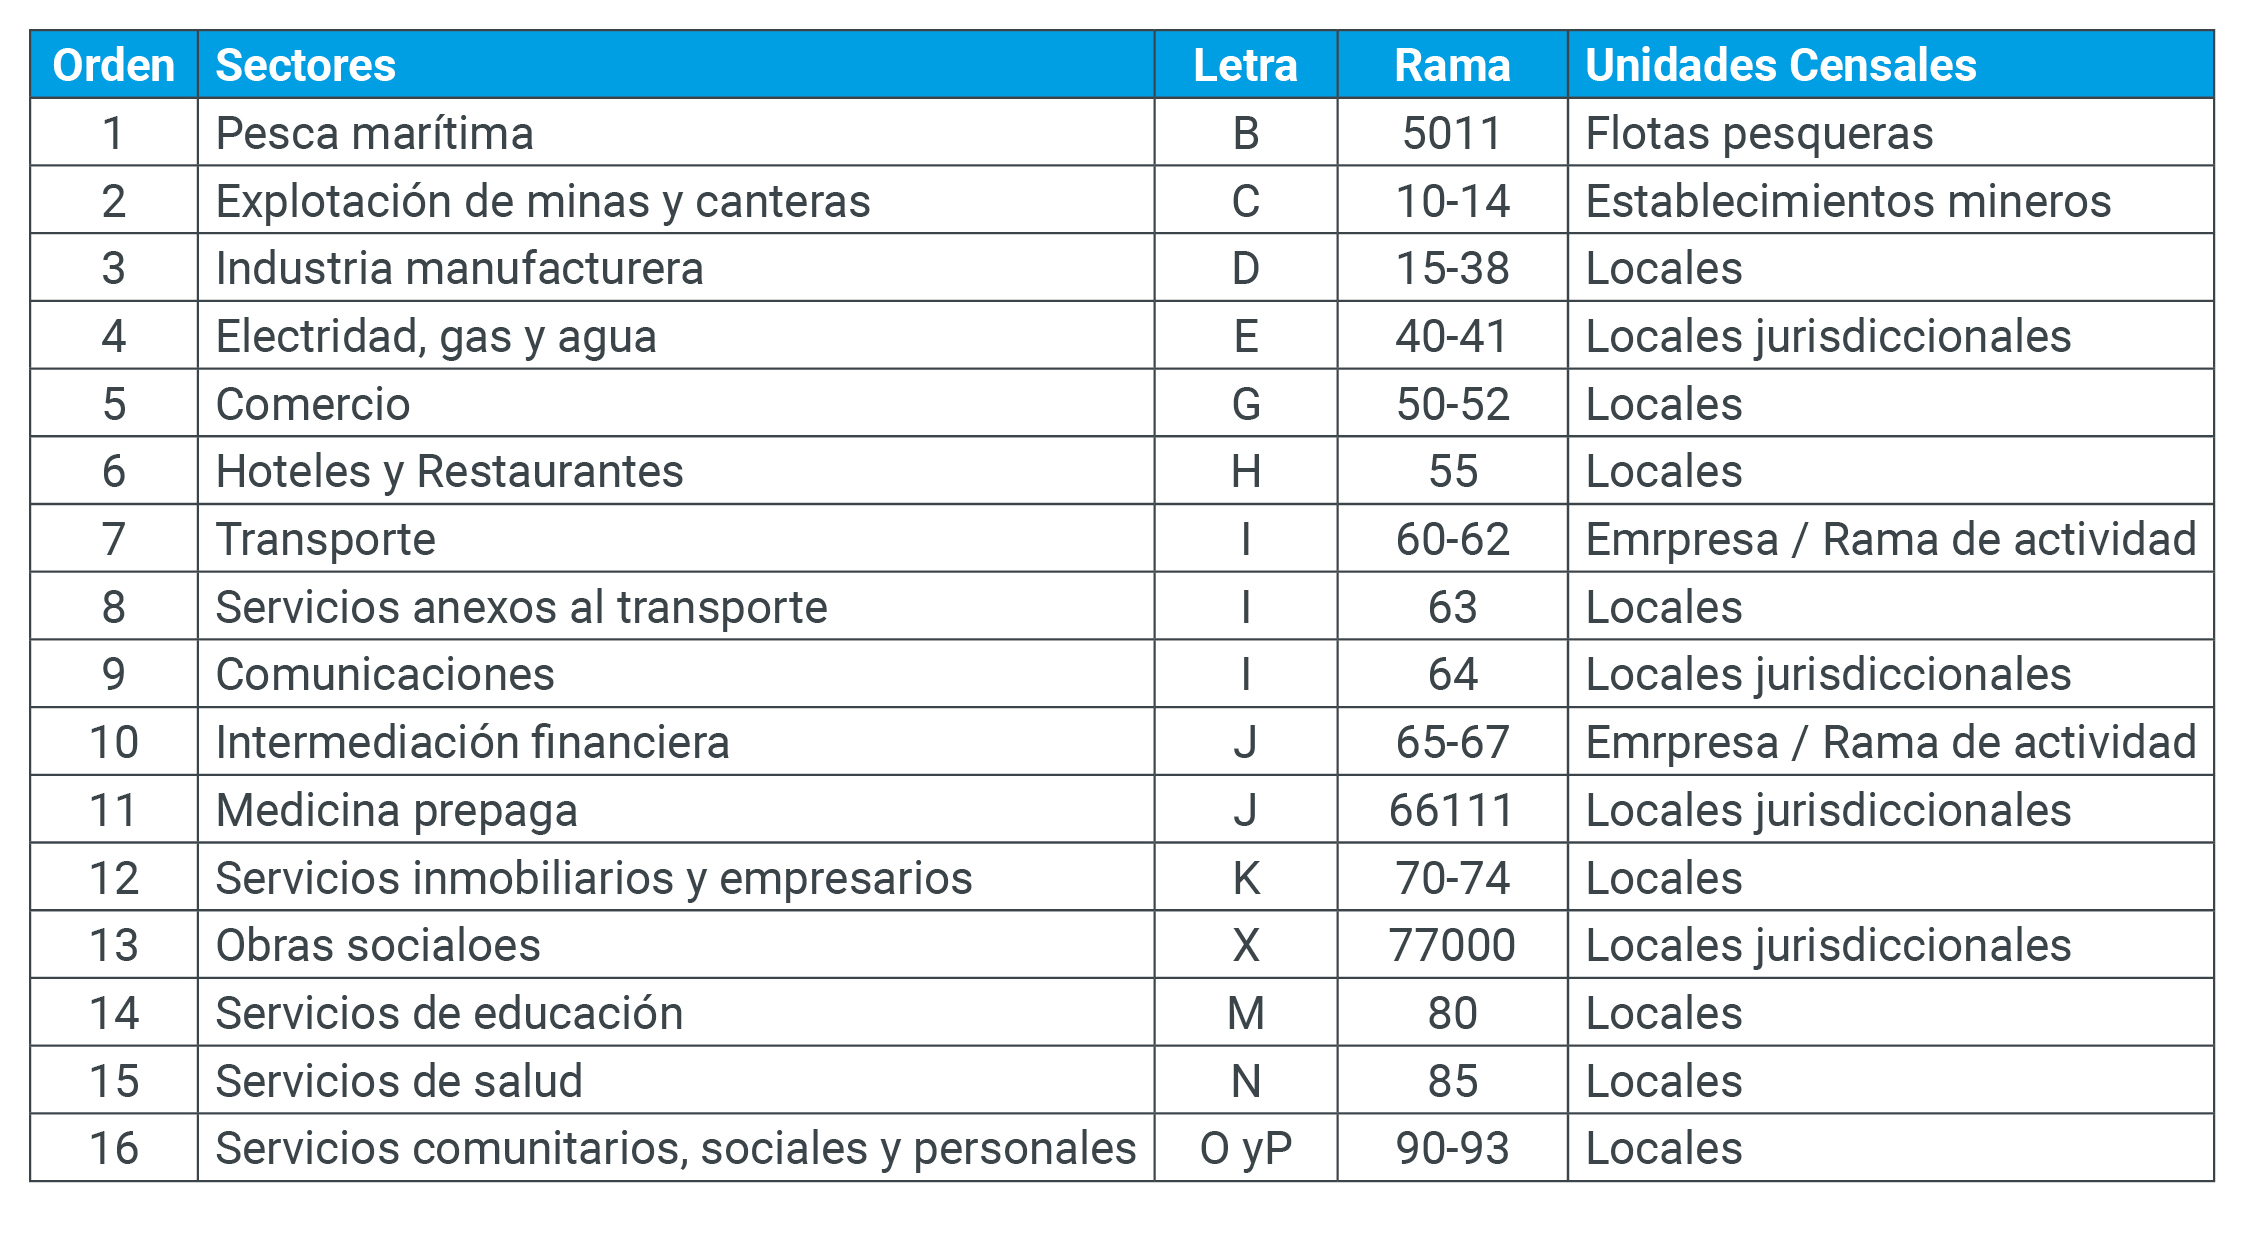
\includegraphics[width=1\linewidth]{imagenes/figura3.12} 

}

\caption{Clasificación de las actividades económicas incluidas en el CNE 2004}\label{fig:empleofuentes12}
\end{figure}

Tal como se desprende del cuadro precedente, el operativo no incluye las actividades de Agricultura, ganadería y caza; ni la Administración pública nacional, provincial y municipal, ni los Organismos internacionales y los servicios domésticos en casa particulares. En el caso particular de las actividades de Transporte y Construcción, sólo se censaron aquellos locales correspondientes a las administraciones centrales. Esto último se encuentra vinculado con las diferencias que se presentan entre la etapa de relevamiento y la correspondiente al censo. Si bien se empadronan tanto a las actividades principales como auxiliares\footnote{Las actividades auxiliares se llevan a cabo sólo como apoyo a las actividades principales y secundarias de la empresa. Las actividades auxiliares son tareas de carácter universal demandadas por todas las ramas de actividad y que las empresas suelen realizar para sí mismas con personal propio, como por ejemplo administración general de la empresa, liquidación de sueldos, asesoría legal, centro de informática, depósito, taller de reparación de la flota de vehículos propios y otras actividades cuyos costos se cubren con los ingresos de las actividades productivas que se llevan a cabo en otros locales de la empresa.}, en los casos de Transporte y Construcción, sólo se censaron las primeras.

En lo referido a la cobertura del operativo, se debe aclarar que las localidades con menos de 1.000 habitantes no fueron relevadas\footnote{Este límite es variable, ya que algunas provincias resolvieron el relevamiento completo de las áreas pobladas.}.

En cuanto a las variables relevadas por un CNE, referidas a actividad económica, son \textbf{VBP}, \textbf{consumo intermedio} y \textbf{VAB}. En el caso del VBP y el VAB se debe tener en consideración el precio al que son valuados, ya que el mismo indica la existencia de impuestos en la valuación del agregado. En el caso del CNE, éstos se encuentran valuados a precios básicos. Éste es el precio recibido por un productor del comprador de una unidad de bien o servicio producido menos cualquier impuesto que lo grave más cualquier subsidio que se reciba como consecuencia de la producción o venta de esa unidad; también excluye cualquier cargo de transporte facturado separadamente por el productor.

En conclusión, es imprtante notar que, a partir de los datos provistos por un CNE, resulta imposible calcular los PGB de las unidades bajo estudio, con un nivel de desagregación óptimo para la estimación de la actividad turística. Esto es porque:

\begin{itemize}
\tightlist
\item
  es preciso contar con información de los sectores no contemplados por el CNE: los datos del sector agropecuario se recopilan a través del Censo Nacional Agropecuario y la Encuesta Nacional Agropecuaria (ENA), mientras que los datos de la administración pública en sus tres niveles se obtienen a través de información brindada por ellas mismas.
\item
  no es posible desagregar al sector transporte, fundamental para evaluar la actividad del sector turístico, a nivel departamental. Este mismo inconveniente se presenta en todos los sectores en los cuales el sector transporte se encuentre involucrado. Aunque dicha desagregación se podría obtener a partir de una estimación ponderada, se debe tener presente que no reflejará fielmente la realidad del sector en la unidad geográfica mencionada.
\item
  el CNE es un operativo que solamente se realiza en zonas urbanas de más de 1.000 habitantes; por tanto, quedan excluidas del operativo las áreas urbanas con una población menor a la mencionada y el sector rural.
\end{itemize}

Adicionlamente, en razón de las características del CNE, como relevamiento dirigido a locales, se pueden identificar los siguientes puntos críticos:

\begin{itemize}
\tightlist
\item
  el subregistro del número de locales productivos como resultado de la no visibilidad de unidades que no llegan a ser identificadas por los censistas,
\item
  la subdeclaración de los niveles de producción y de ocupación por parte de los locales efectivamente censados.
\end{itemize}

Sin embargo, a pesar de estas dificultades, los CNE pueden ser una fuente secundaria o alternativa al PGB calculado por las provincias a fin de estimar la contribución económica del turismo en la economía regional/provincial.

En este sentido, se proponen los siguientes pasos a fin de dar utilidad a la información relevada por los CNE:

\begin{enumerate}
\def\labelenumi{\arabic{enumi}.}
\tightlist
\item
  Identificar las ramas turísticas con el mayor nivel de desagregación posible (recordar que en la figura \ref{fig:activcst} se detallan las RCT con su máximo nivel de desagrgación según el CLANAE 2004 y el CLANAE 2010).
\item
  Para los casos provinciales en donde el nivel de agregación sea muy alto (2 dígitos del CLANAE por ejemplo), se pueden aplicar las estructuras de desagregación del total país para cada rama de actividad, a fin de abrirlas y estimar más precisamente el componente turístico. O bien, se puede utilizar información propia de la provincia para desagregar las ramas en sus diferentes subramas.
\item
  Imputar las ramas que se presentan sin información por secreto estadístico\footnote{El secreto estadístico (SE) se utiliza para proteger el anonimato de los informantes, por lo que cuando en una desagregación determinada (por rama y/o geográfica) en un casillero quedan una o dos empresas, se informa únicamente el número de locales, pero no las otras variables.}. La estrategia propuesta en este caso consiste en: calcular la diferencia, de cada variable a imputar, entre el valor para el total país y la suma de las provincias sin SE. Esto arroja la cantidad de la variable a distribuir entre aquellas que presentan SE. Luego de estimar dicha cantidad, se distribuye linealmente de acuerdo a la participación de los locales de una provincia determinada sobre el total de los locales de provincias afectadas por el SE.
\item
  Cálculo del indicador VAB de las industrias turísticas y proporción sobre el total de la economía: cociente entre la suma de los VAB de las RCT y la suma de los VAB de la economía provincial. Aquí es importante notar que el total de la economía será aquel correspondiente a lo relevado por el CNE y no al total que podría obtenerse de la estimación integral que realiza un PGB.
\end{enumerate}

\textbf{Censo Nacional Económico 2020/2021}

Si bien los puntos mencionados son pertinentes para la última versión disponible del CNE, el nuevo censo que se está llevando a cabo tiene un abordaje metodológico diferente al anterior, así como nuevos procedimientos, que intentan resolver algunos de los puntos críticos del enfoque previo, a la vez que pueden surgir nuevos.

Algunos puntos para destacar del nuevo operativo, que lo diferencian del anterior son:

\begin{itemize}
\tightlist
\item
  Define como unidad estadística a la ``empresa'' y no al ``local''.
\item
  Empadronamiento digital a través de un sitio web, mediante un formulario a ser completado por los agentes económicos (empresas, ISFL, monotributistas y autónomos), reemplazando el barrido territorial de establecimientos productivos y entrega de los formularios censales.
\item
  Complemento de la información con datos agregados a nivel sectorial provenientes de la AFIP
\item
  Encuestas estructurales digitales por muestreo para obtener información de producción e insumos desagregados por actividad y producto, canales y márgenes de transporte y comercio, entre otros.
\end{itemize}

Visite la página oficial del Censo Nacional Económico \href{https://censoeconomico.indec.gob.ar/}{aquí}

\ldots\ldots\ldots\ldots\ldots\ldots\ldots\ldots\ldots\ldots\ldots\ldots\ldots\ldots\ldots\ldots\ldots\ldots\ldots\ldots\ldots\ldots\ldots\ldots\ldots{}

\hypertarget{mediciuxf3n-del-empleo-provincial-caracteruxedsticas-de-las-fuentes-disponibles}{%
\section{Medición del empleo provincial: características de las fuentes disponibles}\label{mediciuxf3n-del-empleo-provincial-caracteruxedsticas-de-las-fuentes-disponibles}}

Esta sección describe las fuentes disponibles para medir el empleo en ramas turísticas, teniendo en cuenta que cada una permite cubrir aspectos diferentes en cuanto a cobertura geográfica, categoría ocupacional -asalariado o independientes de distinto tipo-, calidad del empleo -grado de formalidad de los trabajadores-, unidad de análisis -puestos de trabajo o trabajadores-, entre otros.

\hypertarget{censo-nacional-de-poblaciuxf3n-hogares-y-vivienda-cnphv}{%
\subsection{Censo Nacional de Población Hogares y Vivienda (CNPHV)}\label{censo-nacional-de-poblaciuxf3n-hogares-y-vivienda-cnphv}}

El \textbf{CNPHV} es llevado a cabo por el Instituto Nacional de Estadística y Censos (INDEC) cada diez años (aproximadamente).

En su condición de operativo de carácter masivo, resulta un instrumento adecuado para la captación de la actividad económica en situaciones económico-sociales de mayor estabilidad y en las que predominan relaciones laborales formales, regulares y estables (por la complejidad que implica la medición de la situación ocupacional de la población en situaciones de irregularidad).\\

Si bien una de las ventajas del CNPHV es su amplia cobertura, una limitación es que transcurridos varios años luego de su realización los datos de empleo y desempleo se encuentran desactualizados.

Como se mencionó arriba, la última información disponible corresponde al CNPHV 2010, con información a nivel provincial de ocupación por rama agrupada y carácter de la ocupación.
Asimismo el CNPHV 2020 fue postergado con motivo de la emergencia sanitaria producto del COVID-19.

Un aspecto no menor es que el CNPHV considera a las personas, ocupadas o no, por la ubicación de su vivienda y las clasifica de acuerdo a su ocupación principal (independientemente de los puestos de trabajo que ocupe).

Por lo tanto, si se quisiera conocer la cantidad de puestos de trabajo, esta fuente no permite realizar tal estimación.

Por último, el CNPHV da cuenta de todas las personas ocupadas, independientemente de la categoría ocupacional (asalariado o empleado, cuentapropista, patrón), de la formalidad de la ocupación (a partir de la realización de aportes, sin distinguir si corresponden a descuentos o aportes realizados por la persona) y del ámbito (estatal o privado), así como de las ramas de actividad a las que corresponde el establecimiento en que trabaja la persona ocupada.

Por último, retomando un punto mencionado más arriba, es preciso señalar que si bien el carácter censal de los datos provenientes de esta fuente pueden hacer suponer que la calidad de los mismos es superior a los datos provenientes de encuestas por muestreo, esto no necesariamente es así.

Al ser un censo un operativo simultáneo y masivo, cientos de miles de personas participan como censistas y, por lo tanto, su capacitación resulta incomparable con la que reciben unos pocos cientos de personas, profesionales en la materia, que de modo continuo relevan información en hogares; particularmente, la medición del mercado de trabajo implica una importante complejidad conceptual.

Así, por ejemplo, el CNPHV del 2001 sobreestimó cerca de un 50\% la desocupación en los grandes aglomerados urbanos (frente a la tasa que surgía en ese periodo de la EPH), por clasificar como desocupados a personas que desde las definiciones que regulan la producción de estadísticas de mercado de trabajo a nivel internacional debían ser señaladas como ocupados (personas que trabajaban pocas horas, que se dedicaban a hacer ``changas'' sin horario ni carga de trabajo fija, etc.).

\hypertarget{censo-nacional-econuxf3mico-cne-1}{%
\subsection{Censo nacional económico (CNE)}\label{censo-nacional-econuxf3mico-cne-1}}

El \textbf{CNE} provee información básica para una descripción detallada de la estructura productiva del país, tanto a nivel nacional, como a nivel provincial y de áreas menores.

Con relación al empleo, el mismo está medido por los puestos de trabajo ocupados por asalariados y no asalariados.

Esto significa que contempla que una misma persona puede tener más de una ocupación, a diferencia del CNPHV, que mide solo personas ocupadas. Sin embargo, no permite conocer cuántas personas ocupan esos puestos de trabajo, puesto que en una porción no desdeñable una persona ocupa dos, e incluso, más puestos.

Asimismo, en el concepto de puestos de trabajo no se incluye al personal de agencias de personal temporario y a las personas físicas contratadas en el local que cobran por factura y trabajan bajo la dirección de la empresa. Los pagos correspondientes, en estos últimos casos, forman parte del consumo intermedio, ya que constituye un servicio de terceros.

Tal como se mencionó anteriormente, ebe recordarse que los Censos Económicos no incluyen información sobre el sector agropecuario que cuenta con un operativo especial y que en particular el CNE 2004 no contó con los datos relevados por el operativo censal correspondientes al Sector Construcción (Letra F del CLANAE 2004) y a la Rama de Actividad Transporte Automotor de Carga (Rama 60210 del CLANAE 2004).

\hypertarget{encuesta-permanente-de-hogares-eph}{%
\subsection{Encuesta Permanente de Hogares (EPH)}\label{encuesta-permanente-de-hogares-eph}}

La \textbf{EPH} es un operativo especialmente diseñado para medir la situación de la población en relación con el mercado de trabajo y describir con precisión las características de la fuerza de trabajo, en el cual trabajan regularmente encuestadores capacitados en los conceptos intrínsecos de un instrumento de medición específico.

Por ello, si bien como cualquier estudio por muestreo está sujeto a diferentes niveles de error estadístico, la calidad de la información recolectada garantiza la casi inexistencia de errores no estadísticos (habituales en los censos de población, por ejemplo, llevados a cabo por una vasta cantidad de censistas con una capacitación muy reducida).

La EPH es un programa nacional de producción sistemática (con ondas trimestrales) y permanente de indicadores sociales realizada por el INDEC y las direcciones de estadística provinciales, que permite conocer las características socioeconómicas y demográficas de la población en los principales centros urbanos del país.

Es una encuesta de propósitos múltiples que releva información sobre hogares y personas en torno a las siguientes temáticas: situación laboral, características demográficas básicas (edad, sexo, etcétera), características migratorias, habitacionales, educacionales e ingresos.

El alcance de la EPH comprende alrededor del 70\% de la población urbana y poco más del 60\% de la población nacional.

La unidad de registro es por persona ocupada, clasificada de acuerdo a su lugar de residencia.

La cobertura geográfica alcanza a 31 aglomerados urbanos del país.

Desde el año 2003 hasta el segundo trimestre de 2006 se relevaban 28 aglomerados urbanos; a partir del tercer trimestre de 2006, con la incorporación de San Nicolás -- Villa Constitución, Viedma -- Carmen de Patagones y Rawson -- Trelew, se amplió la cobertura de la encuesta a 31 centros urbanos.

\hypertarget{eph-total-urbano}{%
\subsection{EPH Total Urbano}\label{eph-total-urbano}}

Este operativo es una ampliación de la cobertura territorial de la EPH. Permite contar con la misma información que en la EPH pero para el total de la población urbana del país, a través de la incorporación a la muestra de los hogares pertenecientes a localidades de 2.000 y más habitantes.

Se realiza en la onda correspondiente al tercer trimestre de la EPH y su cobertura alcanza al 90\% de la población total del país.

La información obtenida puede ser desagregada para cada gran aglomerado urbano y para los restos urbanos provinciales (es decir, población urbana sin contar los residentes en el o los grandes aglomerados).

Se encuentra disponible para el período 2010-2014 como Encuesta Anual de Hogares Urbanos (EAHU) y a partir de 2016 como EPH total urbano.

\hypertarget{sistema-integrado-previsional-argentino-sipa}{%
\subsection{Sistema Integrado Previsional Argentino (SIPA)}\label{sistema-integrado-previsional-argentino-sipa}}

La información básica a partir de la cual se captan los datos del \textbf{SIPA} proviene de las declaraciones juradas realizadas por las empresas.

Las empresas se clasifican por actividad económica según cómo se inscriban en la AFIP.
Dicha inscripción se realiza una única vez por cada entidad contribuyente, asignando el CUIT (Código Único de Identificación Tributaria) de acuerdo a la actividad principal que declaran las mismas.

Por diferentes causas, tales como descripción incompleta o incorrecta de la actividad o cambios de la misma a lo largo del tiempo, empresas dedicadas a una misma tarea pueden quedar asignadas a clasificaciones diferentes.

Por esta razón, en su transformación a información estadística se han examinado algunos sectores recodificando la actividad original (estos ajustes son realizados para la información publicada por el Ministerio de Trabajo, Empleo y Seguridad Social -MTEySS-).

El SIPA es un sistema que contabiliza a las personas físicas mayores de 18 años de edad que desempeñan alguna actividad como asalariados y a los que sus empleadores les realizan los aportes previsionales; es decir, sólo alcanza a los puestos de trabajo asalariados del sector privado registrado (es decir, a los que las empresas les realizan los descuentos dirigidos a la seguridad social), dejando por fuera a los trabajadores no englobados en esta categoría (sean asalariados o independientes).

El MTEySS publica mensualmente la evolución de los trabajadores privados registrados a nivel nacional por rama de actividad de la ocupación principal (agrupamiento en 15 ramas), así como la evolución de los asalariados registrados por provincia sin desagregación sectorial.

El Observatorio de Empleo y Dinámica Empresarial (OEDE), dentro del MTEySS, publica la información de asalariados registrados tanto a nivel nacional como provincial con una desagregación a 4 dígitos del CIIU rev. 3 con periodicidad trimestral (en algunos casos, como Servicio de transporte ferroviario, la desagregación es a 3 dígitos).

\hypertarget{suxedntesis-comparativa-de-las-fuentes}{%
\subsection{Síntesis comparativa de las fuentes}\label{suxedntesis-comparativa-de-las-fuentes}}

\hypertarget{comparaciuxf3n-de-las-fuentes-disponibles}{%
\subsubsection{Comparación de las fuentes disponibles}\label{comparaciuxf3n-de-las-fuentes-disponibles}}

En la figura \ref{fig:empleofuentes1} se aprecia una síntesis de las principales características de las fuentes de información descriptas a lo largo de la sección anterior, mientras que en la \ref{fig:empleofuentes2} se detallan las principales fortalezas y debilidades de cada una.

\begin{figure}

{\centering 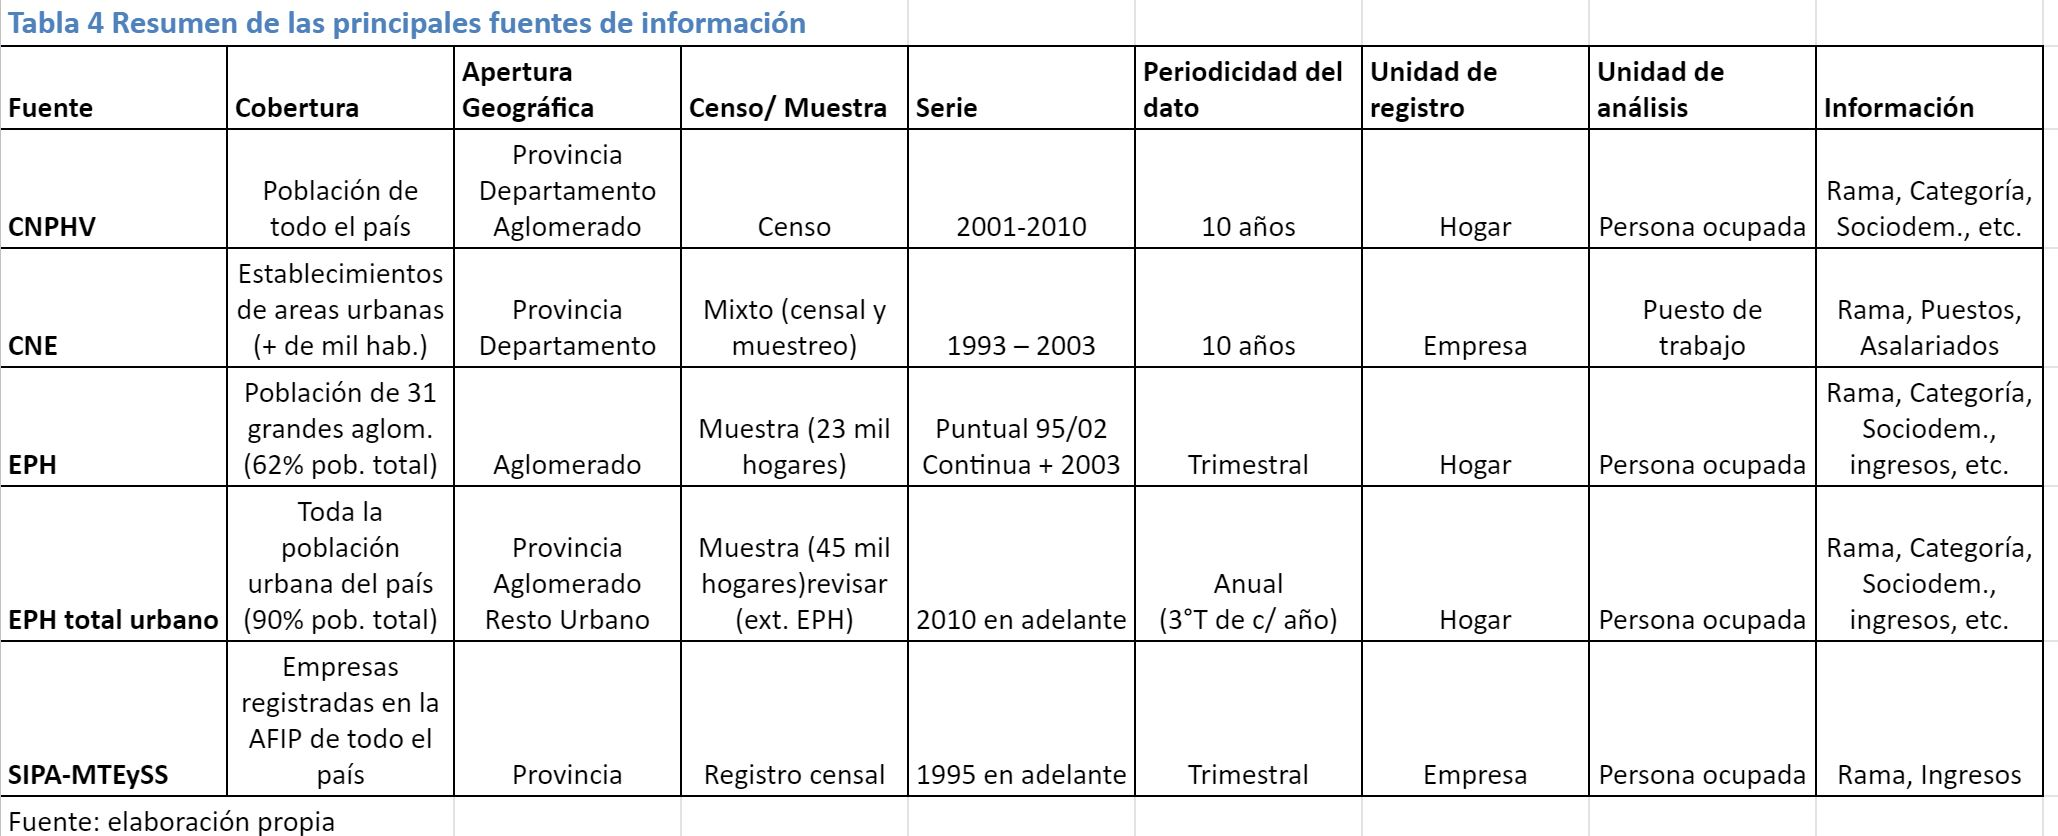
\includegraphics[width=1\linewidth]{imagenes/figura3.1} 

}

\caption{Resumen de las principales fuentes de información}\label{fig:empleofuentes1}
\end{figure}

\begin{figure}

{\centering 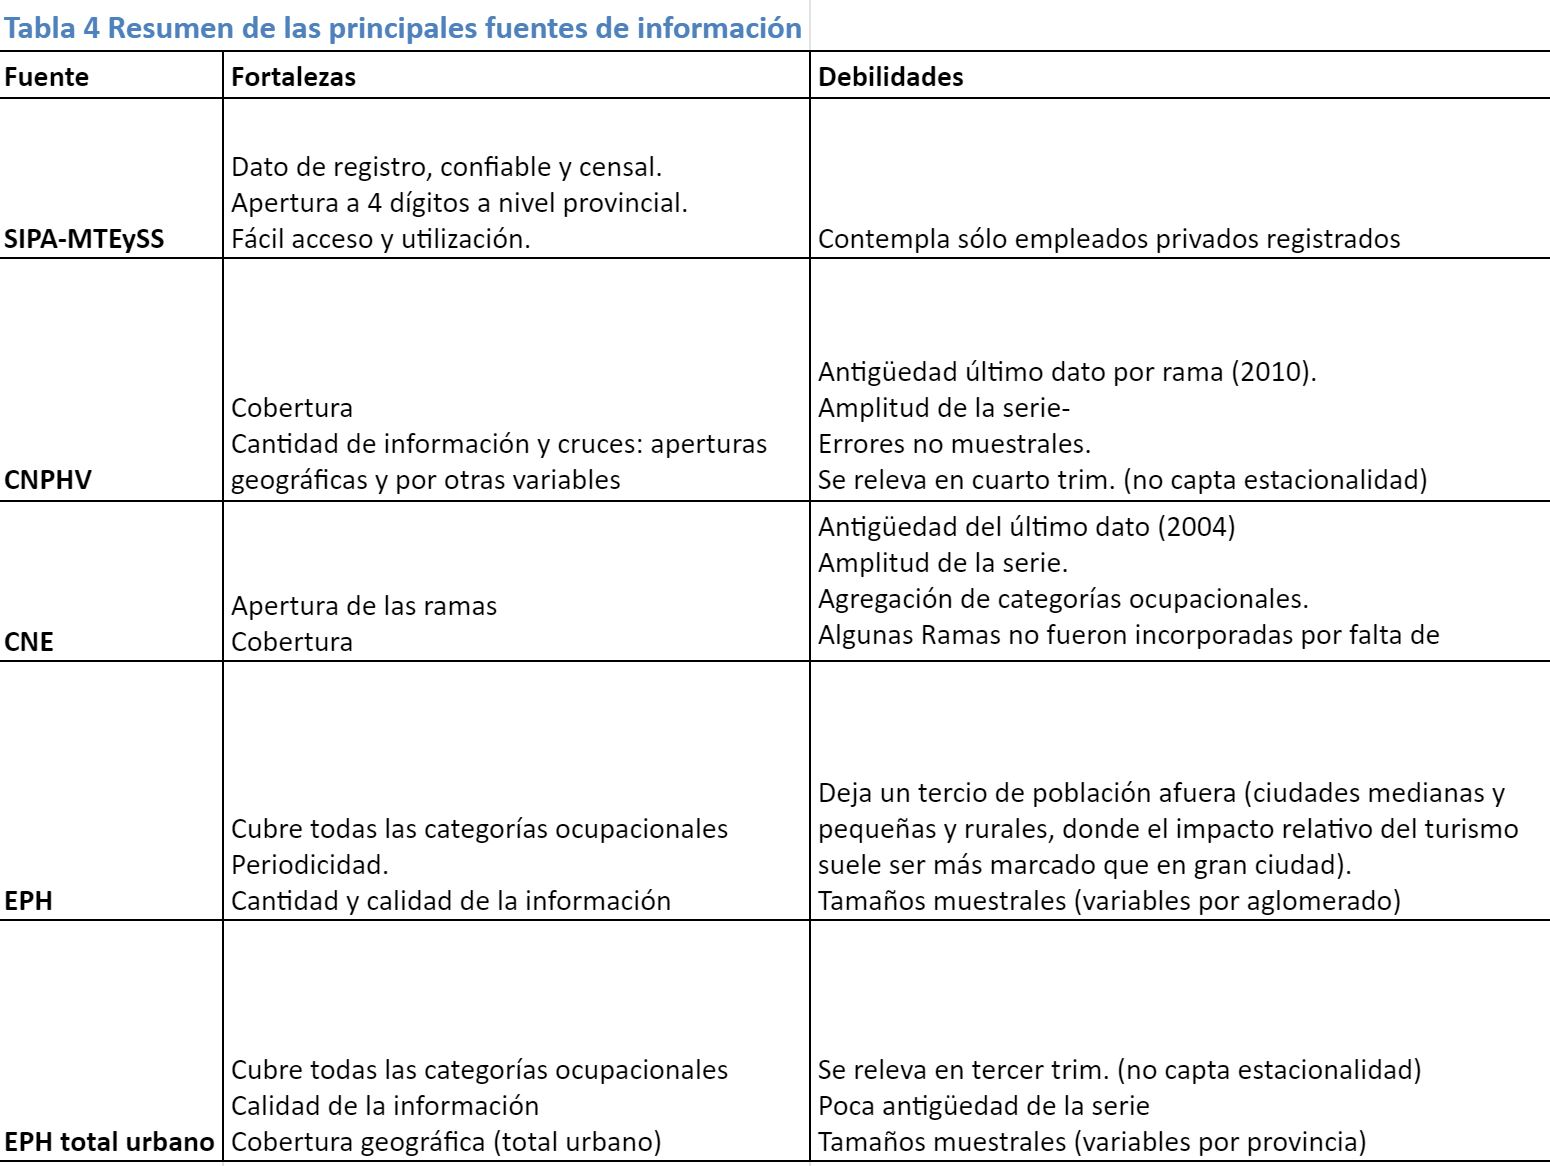
\includegraphics[width=1\linewidth]{imagenes/figura3.2} 

}

\caption{Fortalezas y debilidades de las principales fuentes}\label{fig:empleofuentes2}
\end{figure}

\hypertarget{categoruxedas-ocupacionales}{%
\subsubsection{Categorías ocupacionales}\label{categoruxedas-ocupacionales}}

Como ya se adelantó, la OIT categoriza un empleo según el tipo de contrato de trabajo explícito o implícito del titular con otras personas u organizaciones agrupadas en el CISE, donde se detallan las distintas modalidades vigentes.

El criterio básico utilizado para definir cada grupo de categoría o clasificación ocupacional es del tipo de riesgo económico, un elemento del cual depende exclusivamente la solidez del vínculo entre la persona y el empleo, y el tipo de autoridad que tiene el trabajador sobre el establecimiento.

Cabe señalar que habitualmente la categoría ocupacional refiere al tipo de relación (patrón, cuenta propia, empleado, etc.).

En este caso, en realidad, la categoría ocupacional refleja una tipología que contempla tres variables: la categoría ocupacional propiamente dicha; el ámbito al que corresponde el establecimiento (privado o estatal); y el nivel de formalidad, determinado por la presencia o no de descuentos o aportes previsionales.

Además de las diferencias de cobertura en el universo de ocupados, no todas las fuentes secundarias presentadas exhiben el mismo nivel de apertura de los datos por categoría ocupacional, como puede observarse en la figura \ref{fig:empleofuentes3}.

El SIPA sólo da cuenta del universo de trabajadores asalariados del sector privado a los que se les realizan descuentos jubilatorios.

El CNE alcanza a todo el sector privado, pero no permite distinguir los niveles de formalidad entre trabajadores asalariados y no asalariados.
Las encuestas a hogares y los censos dan cuenta de todos los ocupados, pero su forma de clasificarlos presenta algunas diferencias.

\begin{figure}

{\centering 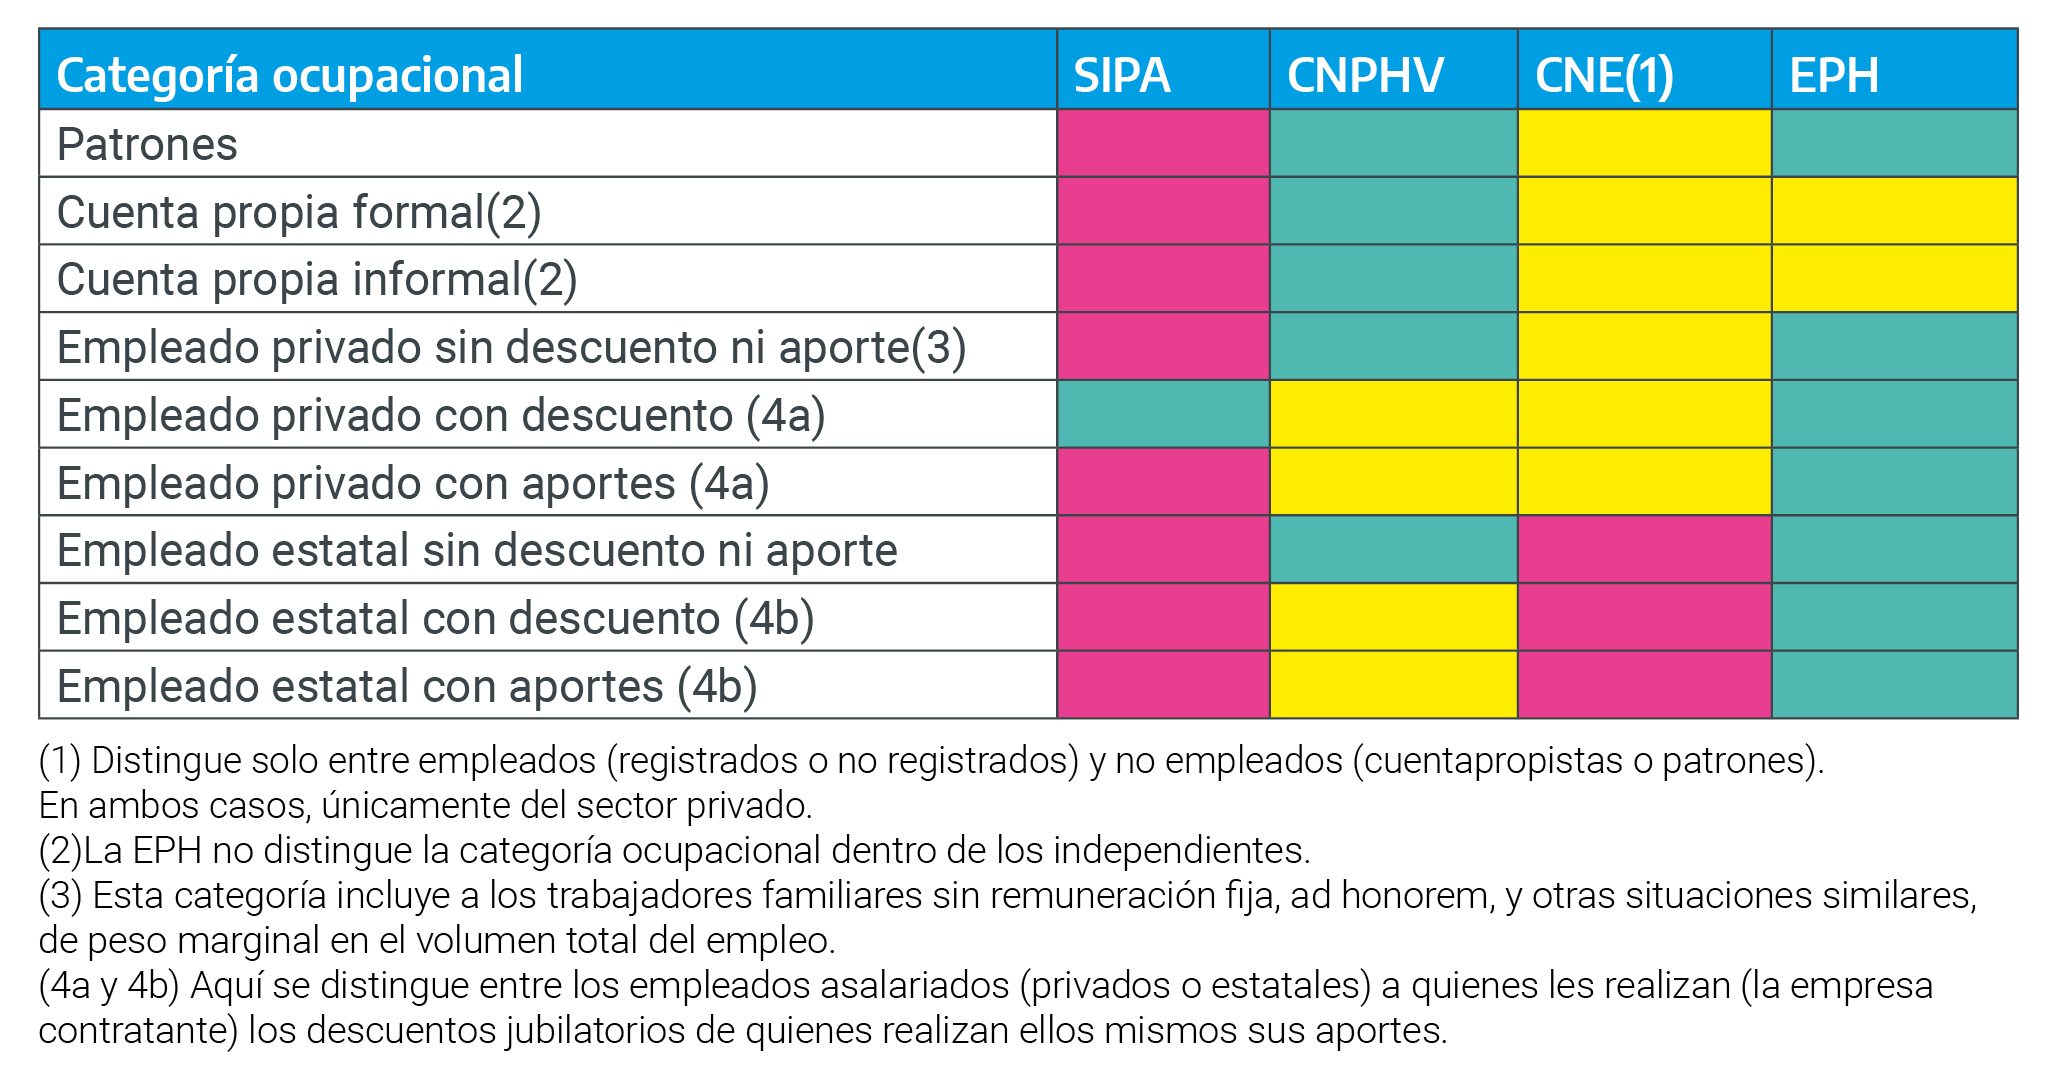
\includegraphics[width=1\linewidth]{imagenes/figura3.3} 

}

\caption{Categoría ocupacional según fuente de información}\label{fig:empleofuentes3}
\end{figure}

Si bien tienen un peso relativamente marginal, la EPH permite distinguir casos de asalariados sin descuento jubilatorio pero con aportes (esto es, una relación de dependencia encubierta), mientras que el CNPHV junta ambas categorías.

En cambio, las encuestas a hogares mencionadas no permiten conocer el nivel de formalidad de trabajadores independientes, mientras que esto sí es posible a partir del Censo, pues la indagación sobre aportes jubilatorios alcanza a todos los ocupados (en las encuestas, solo a los asalariados).

\hypertarget{tipos-de-informalidad}{%
\subsubsection{Tipos de informalidad}\label{tipos-de-informalidad}}

La apertura de la información por categoría ocupacional permite arribar a un aspecto central de la medición del empleo: la informalidad laboral, indicador que permite aproximarse a la calidad del empleo.

Por ello, para complejizar y enriquecer el análisis se han establecido tres tipos de informalidad, en función de la mirada focalizada en distintos segmentos del mercado de trabajo:

\begin{itemize}
\item
  \textbf{Informalidad Total (IT):} Refleja el peso agregado de los cuentapropistas informales y los asalariados del sector privado y estatal sin aportes ni descuentos sobre el total de ocupados.
\item
  \textbf{Informalidad en el Ámbito Privado (ISP):} Considera el peso agregado de los cuentapropistas informales y los asalariados del sector privado sin aportes ni descuentos sobre el total de ocupados del sector privado (excluye a los asalariados del sector estatal).
\item
  \textbf{Informalidad en el Ámbito Privado Asalariado (ISPA):} Refleja la participación de los asalariados del sector privado sin aportes ni descuentos sobre el total de asalariados del sector privado (excluye a los asalariados del sector estatal y a los patrones y cuentapropistas -formales e informales-).
\end{itemize}

\hypertarget{ramas-caracteruxedsticas-ramas-mixtas-y-agregaciuxf3n-de-las-rct-por-sector}{%
\section{Ramas Características, ramas mixtas y agregación de las RCT por sector}\label{ramas-caracteruxedsticas-ramas-mixtas-y-agregaciuxf3n-de-las-rct-por-sector}}

Tal como se explicó en el primer capítulo, cuanto menor sea el nivel de apertura que presente la información por rama, menor será la precisión de los resultados obtenidos.

Esto significa, por ejemplo, que si una determinada fuente brinda únicamente los datos globales a dos dígitos de la CIIU de la Rama Transporte de Servicios Terrestres, la estimación incluirá componentes no relacionados con el turismo, como por ejemplo, el transporte de carga.

En cambio, si la información se presenta en un nivel de detalle mayor, permite discriminar mejor qué es y qué no es característico del sector bajo estudio.

El detalle de las ramas contenidas en cada uno de los sectores turísticos puede apreciarse en la figura \ref{fig:activcst} del capítulo 1. Como allí se observa, no todas las ramas corresponden al mismo nivel de desagregación: en algunos casos se han incluido actividades a tres dígitos, en otros a cuatro y, finalmente, en los casos restantes las actividades corresponden a una clasificación a nivel de cinco dígitos.

Como se mencionó, el nivel de desagregación de las actividades económicas en las fuentes es variable y en una importante cantidad de casos no está presente con la apertura requerida. Para el caso de la medición de la actividad económica de las RCT, su nivel de precisión dependerá de las estadísticas de oferta de cada provincia y su nivel de apertura. Para el caso de la medición del empleo en las RCT, cada una de las fuentes mencionadas posee diferentes niveles de apertura.

Por lo tanto, a continuación se realizará un recorrido por cada una de las ramas para determinar cuánto de lo que hay disponible, para el caso de las fuentes de empleo turístico, se acerca al ideal que establece la CIIU. Para esto, se organizaron las ramas en un esquema de colores semejantes a un semáforo para establecer en qué punto todo el componente es turístico.

Por ejemplo, el sector de Transporte Aéreo incluye la rama ``Servicios de Transporte Aéreo de Pasajeros'' y ``Servicios de Transporte Aéreo de Carga'', donde solo la primera de ellas es una RCT.

Cada uno de los colores en las tablas expresan lo siguiente:

\begin{itemize}
\tightlist
\item
  {\textbf{VERDE:}} Código compuesto por actividades correspondientes en su totalidad a la industria turística.
\item
  {\textbf{AMARILLO:}} Código bajo el cual coexisten tanto componentes de industria turística y de otras actividades económicas no características del turismo.
\item
  {\textbf{ROJO:}} El código no corresponde a una industria turística, aunque si comparte con alguna de estas un código de menor apertura. Adicionalmente, en cada una de las tablas se indica cuál es el código que corresponde a cada fuente, de acuerdo al clasificador considerado en ellas\footnote{La EPH fue objeto de un cambio en el nomenclador de actividades, ya que el vigente hasta 2011 fue reemplazado por una actualización de ese mismo año.}.
\end{itemize}

Es importante notar que para el caso de la fuente CNE (realizado en los años 2004/2005), la misma corresponde a la apertura para el total nacional. Por lo tanto, algunas ramas tendrán información a 3, 4 o 5 dígitos. Sin embargo, es posible que para la apertura provincial no se cuente con tal detalle, sino con una apertura menor. De cualquier manera, las mayores aperturas del total nacional pueden ser utilizadas para elaborar estructuras que puedan aplicarse a los totales provinciales (ver ejemplo en rama Transporte \ref{ejemplo-CNE}).

A su vez, a fin de simplicar la exposición, se han agrupado las RCT en 4 grandes grupos: 1) Alojamiento y Restaurantes, 2) Transporte y 3) Otros servicios turísticos.

\hypertarget{sector-alojamiento-y-restaurantes}{%
\subsection{Sector Alojamiento y Restaurantes}\label{sector-alojamiento-y-restaurantes}}

La rama 55, de la CIIU Rev 3.1, incluye ambos sectores, que se dividen a partir de los tres dígitos.

Ambos sectores presentan una subrama no característica del turismo, cuando se los abre a 5 dígitos.

Dado que todas las fuentes utilizadas, para la medición del empleo turístico, presentan una apertura de como máximo 4 dígitos, a excepción del CNE, habrá una leve sobreestimación del empleo en estas ramas (figura \ref{fig:empleofuentes5}).

\begin{figure}

{\centering 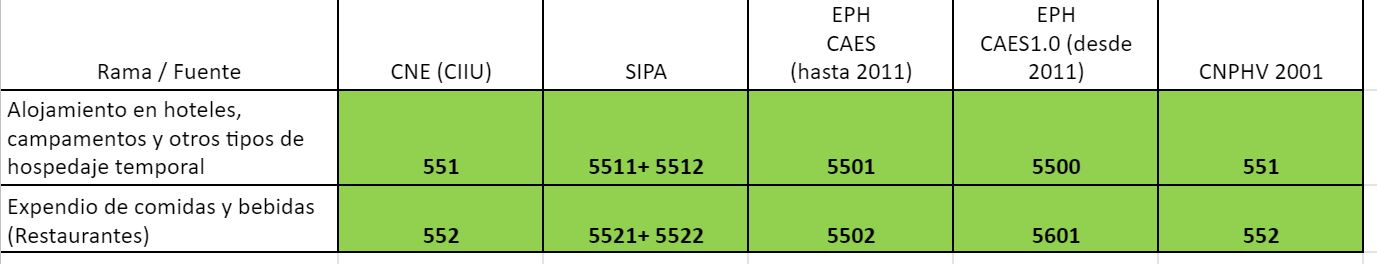
\includegraphics[width=1\linewidth]{imagenes/figura3.5} 

}

\caption{Alojamiento y restaurantes. Clasificación de actividades por fuente}\label{fig:empleofuentes5}
\end{figure}

\hypertarget{sector-transporte}{%
\subsection{Sector Transporte}\label{sector-transporte}}

Los servicios de transporte constituyen una actividad fundamental para la circulación de personas y carga.

En esta sección se incluyen los servicios organizados por cuenta de terceros, sean estos una prestación de tipo colectiva, individualizada o realizada a través del alquiler del vehículo de transporte con su respectivo personal de conducción.

El sector transporte se compone, siguiendo la clasificación a dos dígitos, en 5 subsectores: terrestre, acuático, aéreo, servicios anexos y alquiler de vehículos sin chofer.

El transporte \textbf{terrestre} se desagrega (a tres dígitos) en ferroviario, automotor por carretera y por tuberías (este último no corresponde a una actividad característica del turismo).

A cuatro dígitos, tanto el transporte ferroviario como el automotor se discrimina en carga y pasajeros, mientras que, a 5 dígitos, se especifica qué tipo de servicios de pasajeros se presta (figura \ref{fig:empleofuentes6}).

\begin{figure}

{\centering 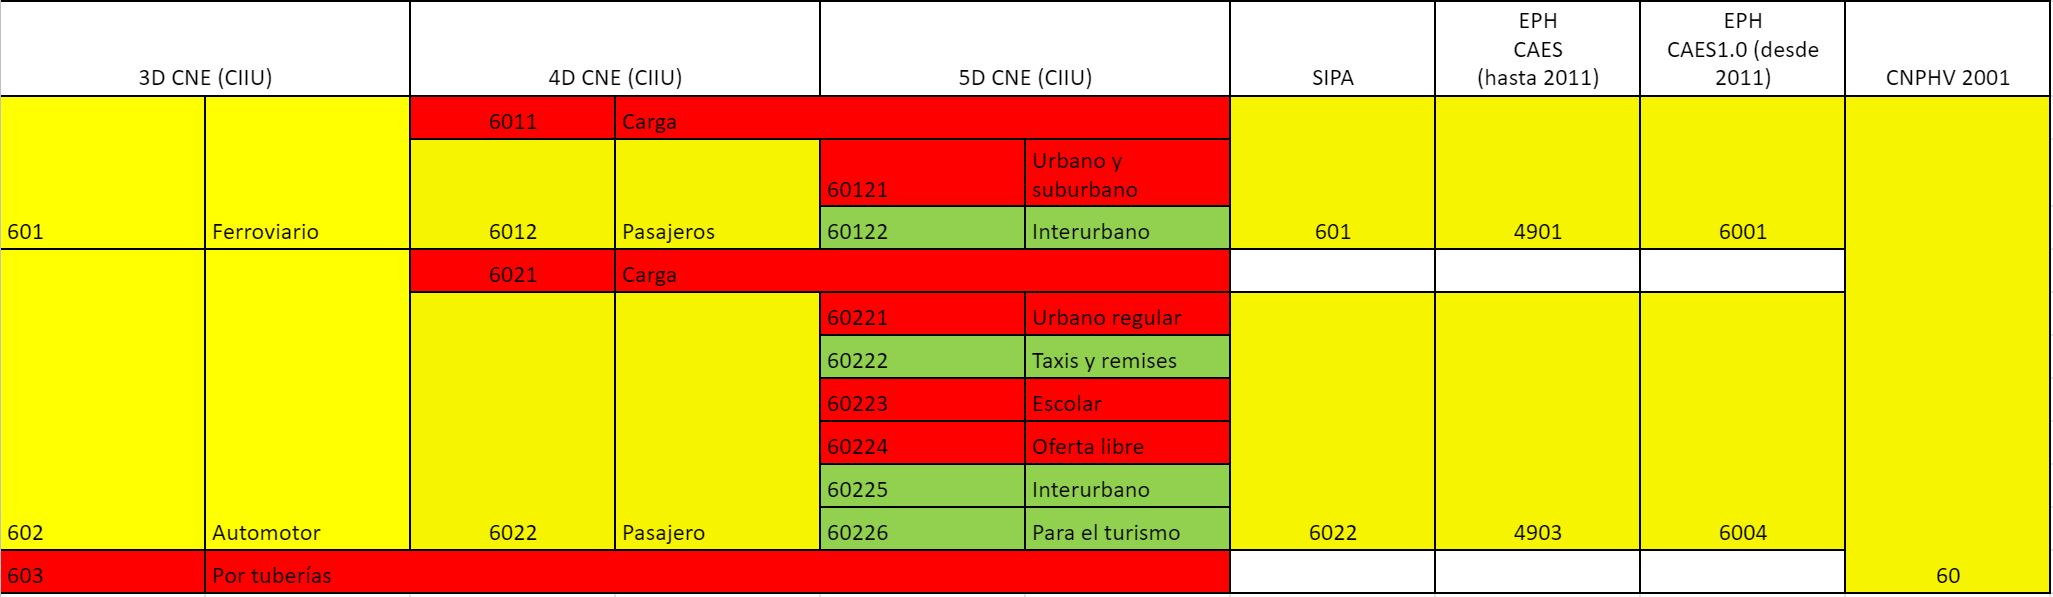
\includegraphics[width=1\linewidth]{imagenes/figura3.6} 

}

\caption{Transporte Terrestre. Clasificación de actividades por fuente}\label{fig:empleofuentes6}
\end{figure}

En el caso del transporte ferroviario, sólo se considera característico el transporte de pasajeros interurbano.

Tanto el SIPA como la EPH presentan la información a tres dígitos (sin discriminar no solo servicios urbanos e interurbanos sino tampoco servicios de carga).

Una forma de aproximar el componente turístico del transporte ferroviario, exluyendo los servicios urbanos y de carga, es obtener un coeficiente que surge del peso relativo de la rama a 5 dígitos ``Transporte interurbano de pasajeros'' sobre la rama ``Transporte ferroviario'', en este caso a partir de la única fuente disponible a 5 dígitos, el CNE 04.
Resulta útil ofrecer un ejemplo para facilitar la comprensión

\hypertarget{ejemplo-CNE}{%
\subsubsection{Ejemplo: Rama Transporte Ferroviario}\label{ejemplo-CNE}}

Según el CNE 2004, los puestos de trabajo correspondientes al transporte ferroviario eran 18.245 y se distribuían de la siguiente forma en la apertura a 5 dígitos del CLANAE 2004:

\begin{itemize}
\tightlist
\item
  \textbf{\emph{5.919}} puestos correspondían a servicio de cargas (6011)
\item
  \textbf{\emph{10.086}} puestos correspondían a servicio de pasajeros urbano y suburbano (60121)
\item
  \textbf{\emph{2.240}} puestos correspondían al servicio de pasajeros interurbano (60122)
  Por tanto, sólo los \textbf{\emph{2.240 puestos}} (pasajeros interurbano) de los \textbf{\emph{18.245}} puestos totales del transporte ferroviario correspondían a actividades características.
\end{itemize}

El coeficiente expresa la participación de los componentes característicos en la suma de todos los componentes involucrados en la desagregación de cada fuente, por lo que en este caso asciende a 0,1228 (2.240/18.245) o, lo que es lo mismo, a 12,28\%.

Así, de los 26.807 puestos de trabajo (asalariados con descuento del ámbito privado) informados por el SIPA para el año 2010 en la actividad transporte ferroviario, 3.227 (cantidad que surge de: 26.807 x 0,1228) serán contabilizados como puestos de trabajos de la actividad característica del sector (servicio interurbano de pasajeros)

En el caso del transporte automotor, los componentes característicos a 5 dígitos son los servicios de taxis y remises (60222), los servicios interurbanos de pasajeros (60225), los servicios internacionales (60227) y los servicios de transporte para el turismo (60226). Siguiendo la lógica planteada, para extraer la cantidad correspondiente a las actividades características del turismo de cada fuente es posible calcular un coeficiente que exprese el peso de las cuatro actividades mencionadas sobre el total de actividades incluidas en el código que las contiene.

Las figuras \ref{fig:empleofuentes7} y \ref{fig:empleofuentes8} presentan el detalle para el transporte acuático y para el transporte aéreo respectivamente.

\begin{figure}

{\centering 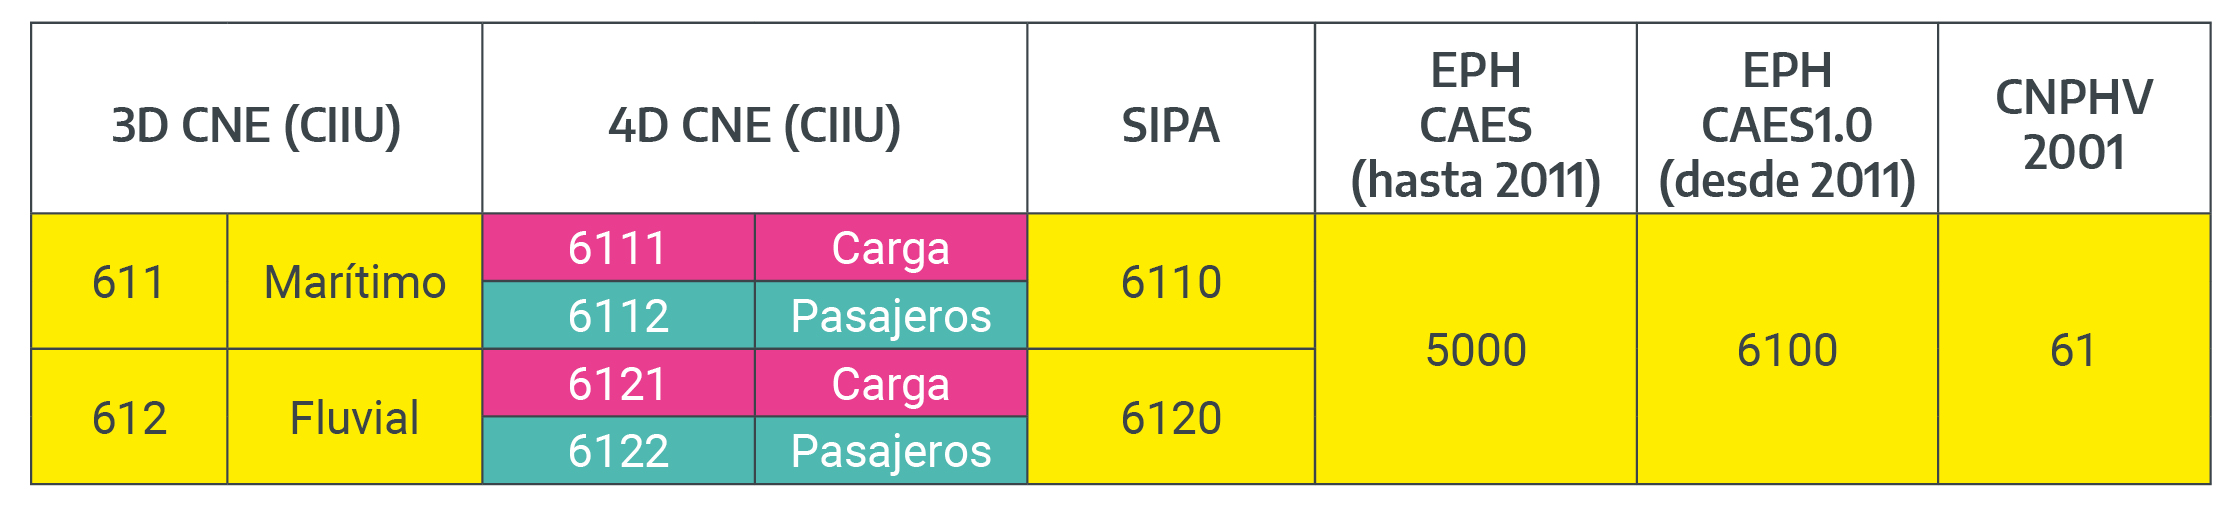
\includegraphics[width=1\linewidth]{imagenes/figura3.7} 

}

\caption{Transporte Acuático. Clasificación de actividades por fuente}\label{fig:empleofuentes7}
\end{figure}

\begin{figure}

{\centering 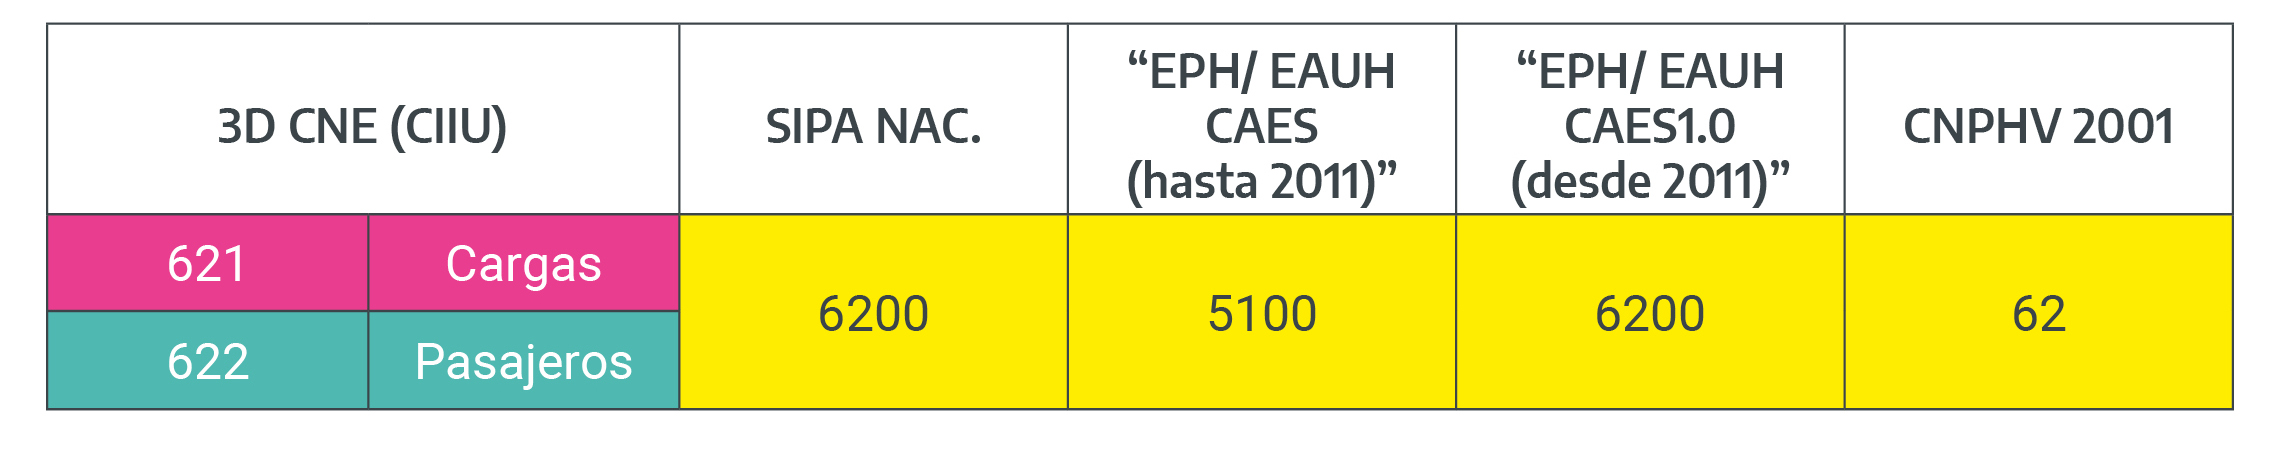
\includegraphics[width=1\linewidth]{imagenes/figura3.8} 

}

\caption{Transporte Aéreo. Clasificación de actividades por fuente}\label{fig:empleofuentes8}
\end{figure}

En la figura \ref{fig:empleofuentes9} se presenta el detalle de la rama 63, que incluye servicios anexos al transporte y agencias de viaje. La actividad de agencias de viaje podría también ser presentada en Otros Servicios Turísticos o como un sector separado. En general, las cuentas nacionales la incluyen dentro de la rama del Transporte, por lo que aquí se siguió esa misma agrupación.

\begin{figure}

{\centering 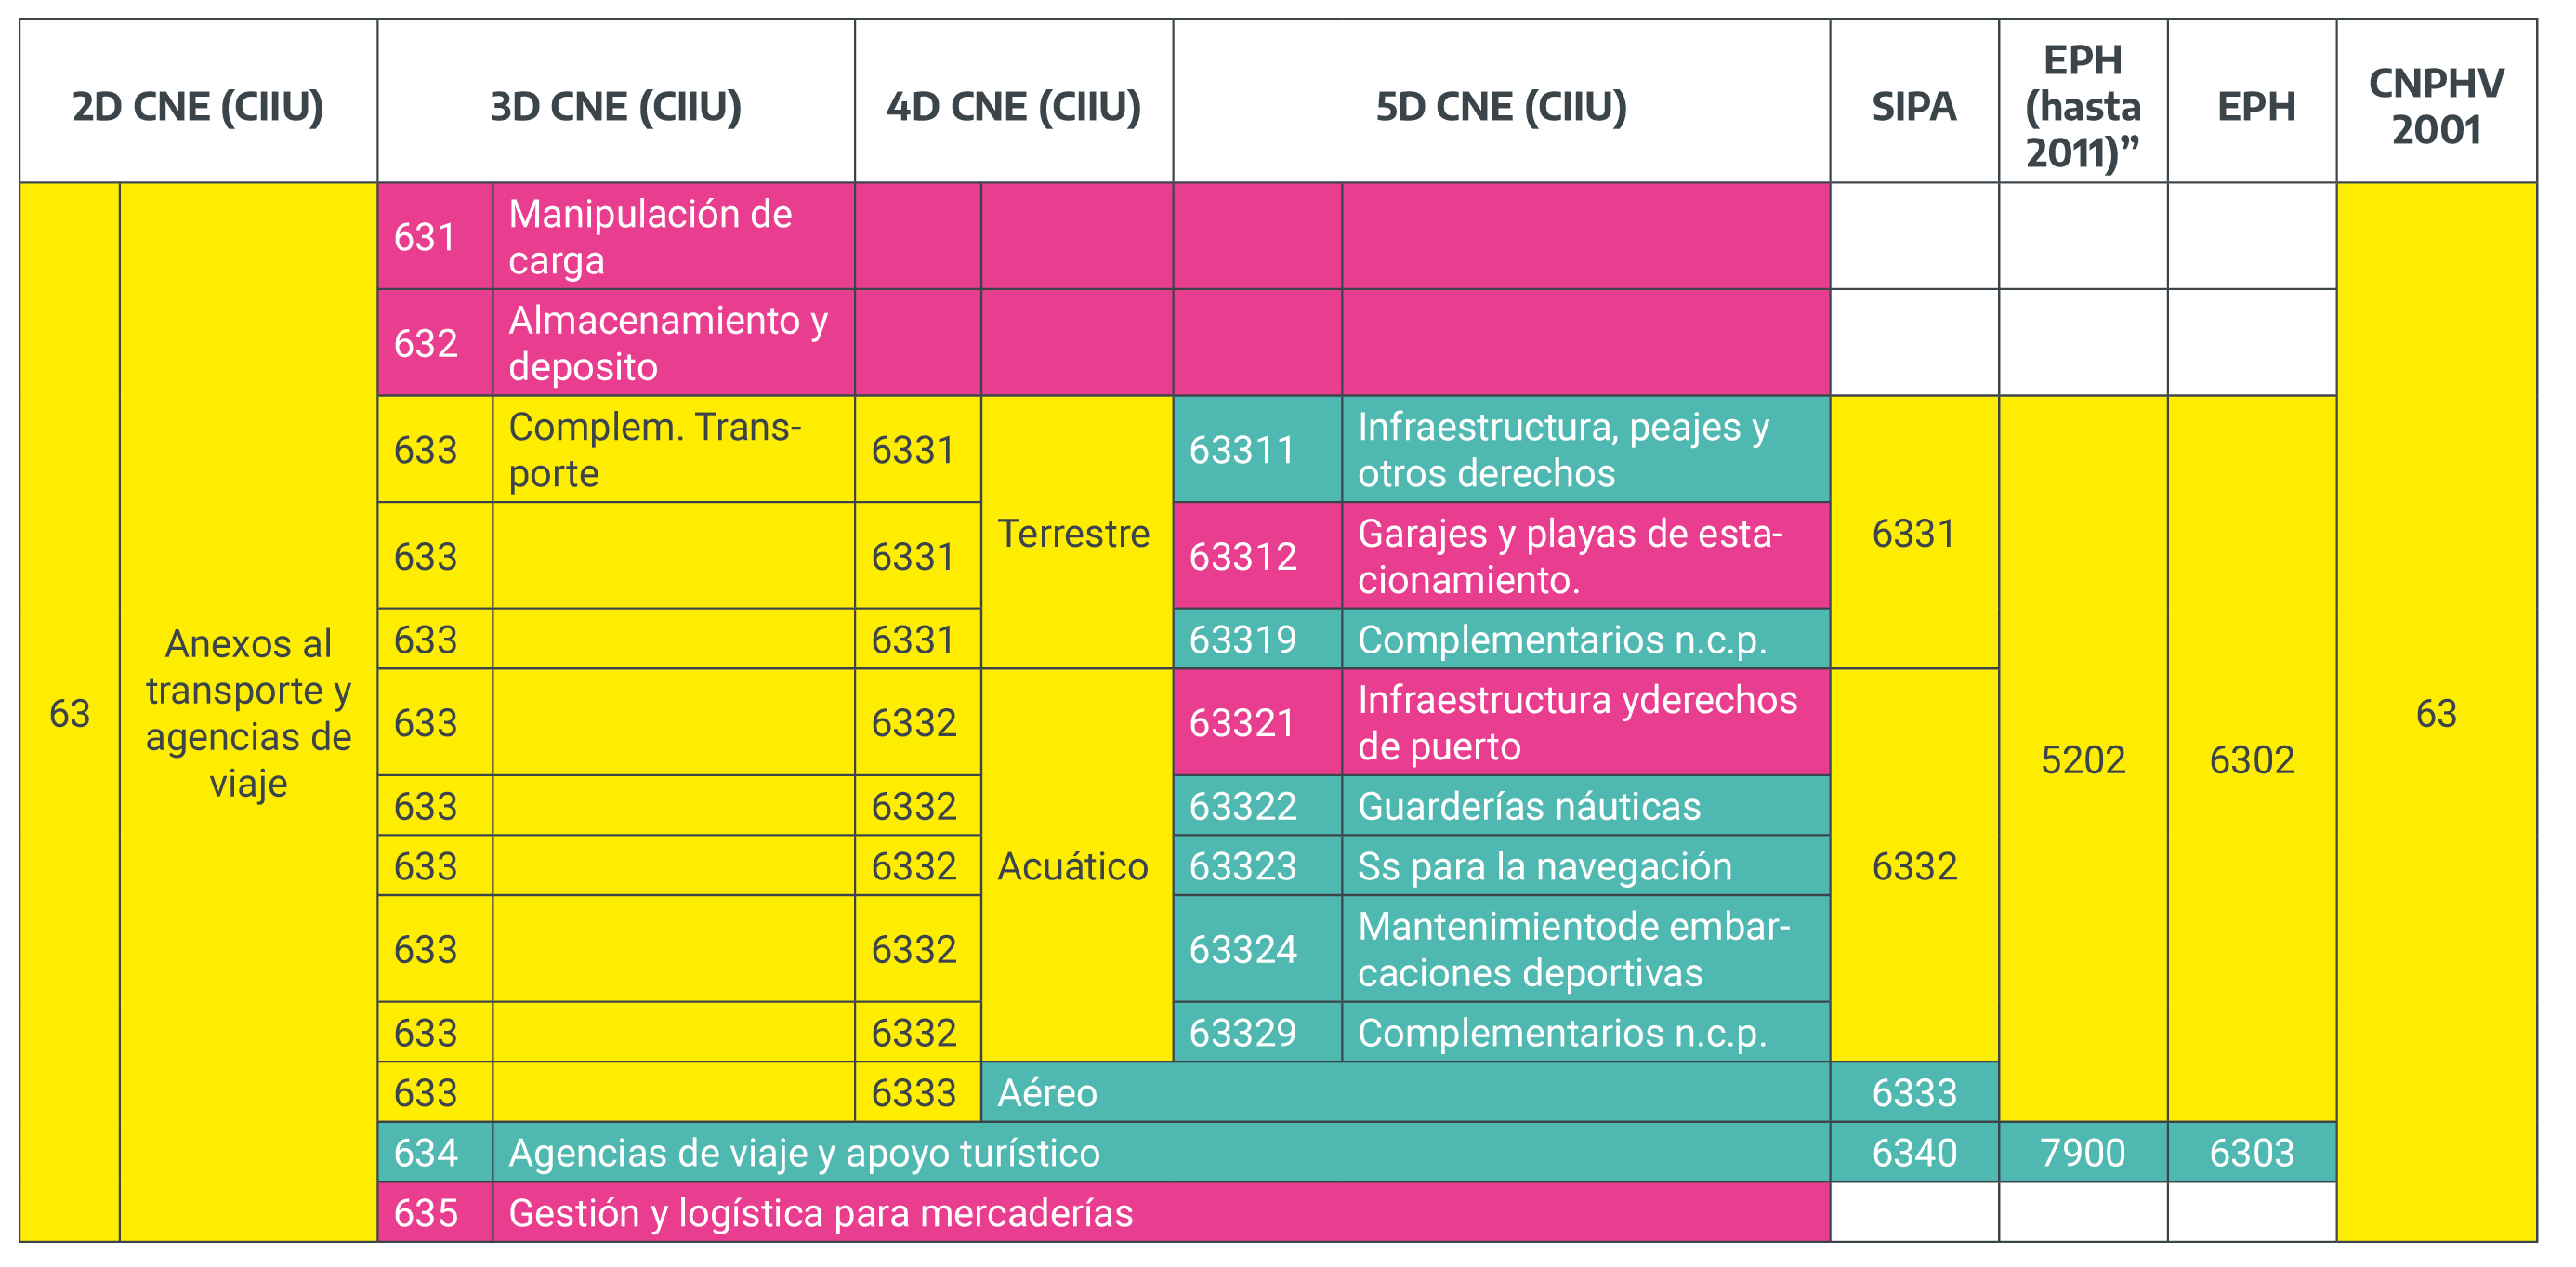
\includegraphics[width=1\linewidth]{imagenes/figura3.9} 

}

\caption{Servicios Anexos al transporte y agencias de viaje. Clasificación de actividades por fuente}\label{fig:empleofuentes9}
\end{figure}

Finalmente, la figura \ref{fig:empleofuentes10} muestra la posición del componente ``Alquiler de transporte sin chofer'' dentro de la rama 71, que incluye el alquiler de transporte, maquinarias y equipos.

\begin{figure}

{\centering 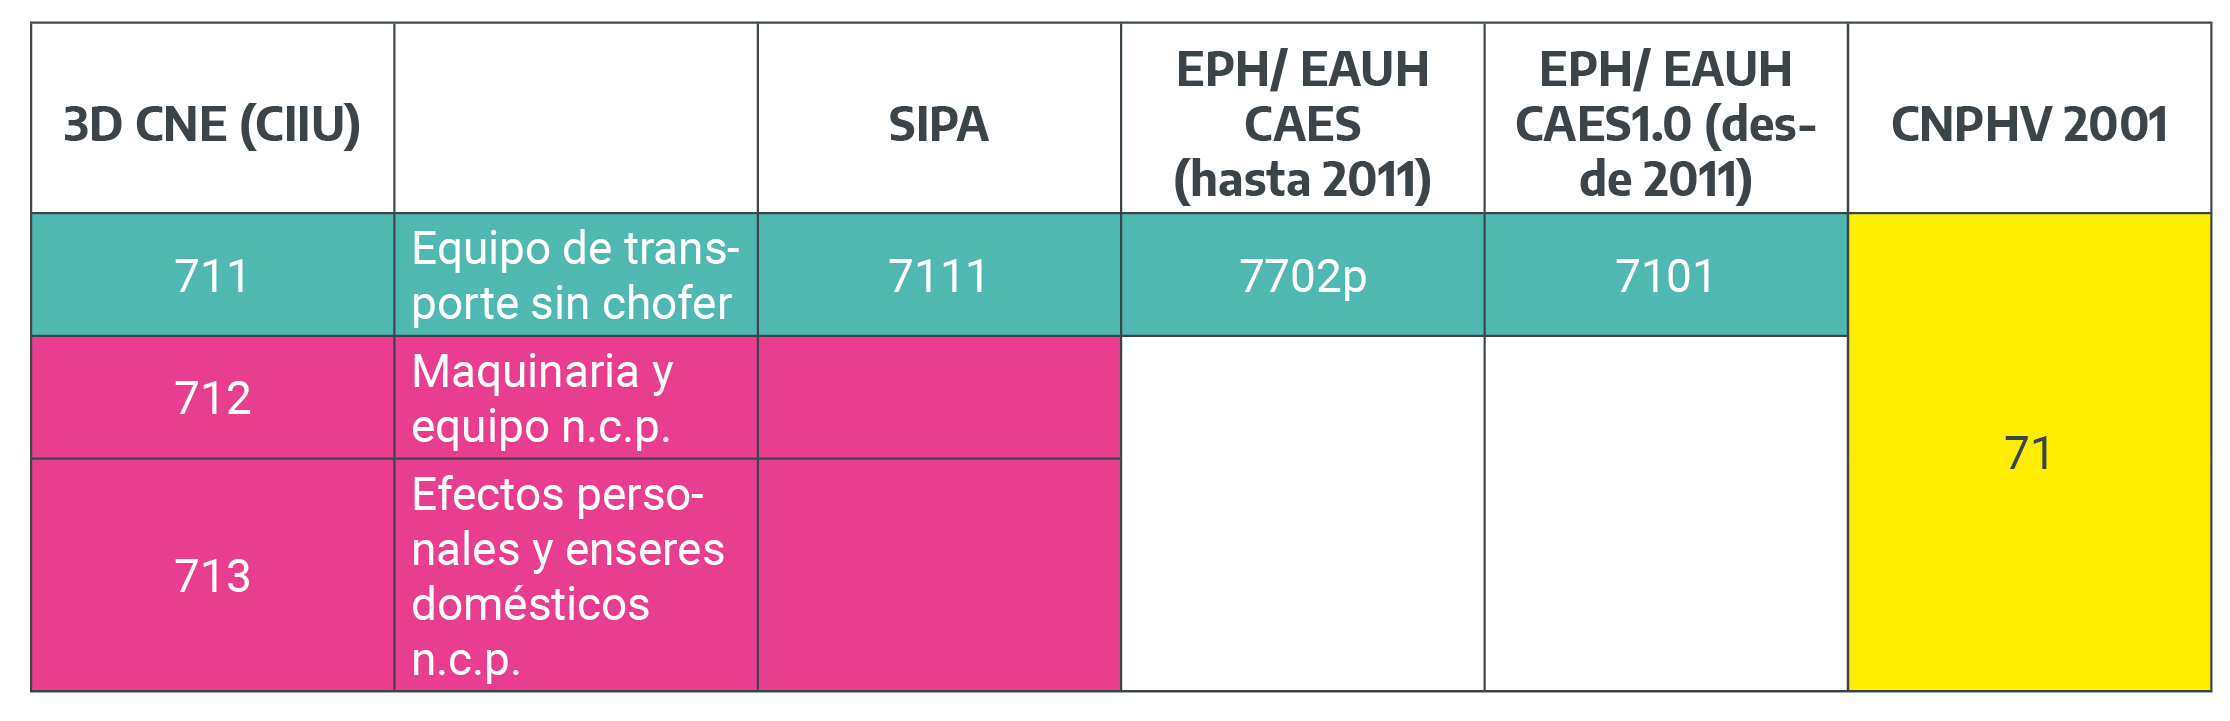
\includegraphics[width=1\linewidth]{imagenes/figura3.10} 

}

\caption{ Alquiler de equipo de transporte, maquinarias y equipo. Clasificación de actividades por fuente.}\label{fig:empleofuentes10}
\end{figure}

\hypertarget{sector-otros-servicios-turuxedsticos}{%
\subsection{Sector Otros Servicios Turísticos}\label{sector-otros-servicios-turuxedsticos}}

Este sector comprende un subconjunto de actividades deportivas, sociales, culturales, recreativas y de interés local agrupadas en la rama 92, del cual da cuenta la \ref{fig:empleofuentes11}.

\begin{figure}

{\centering 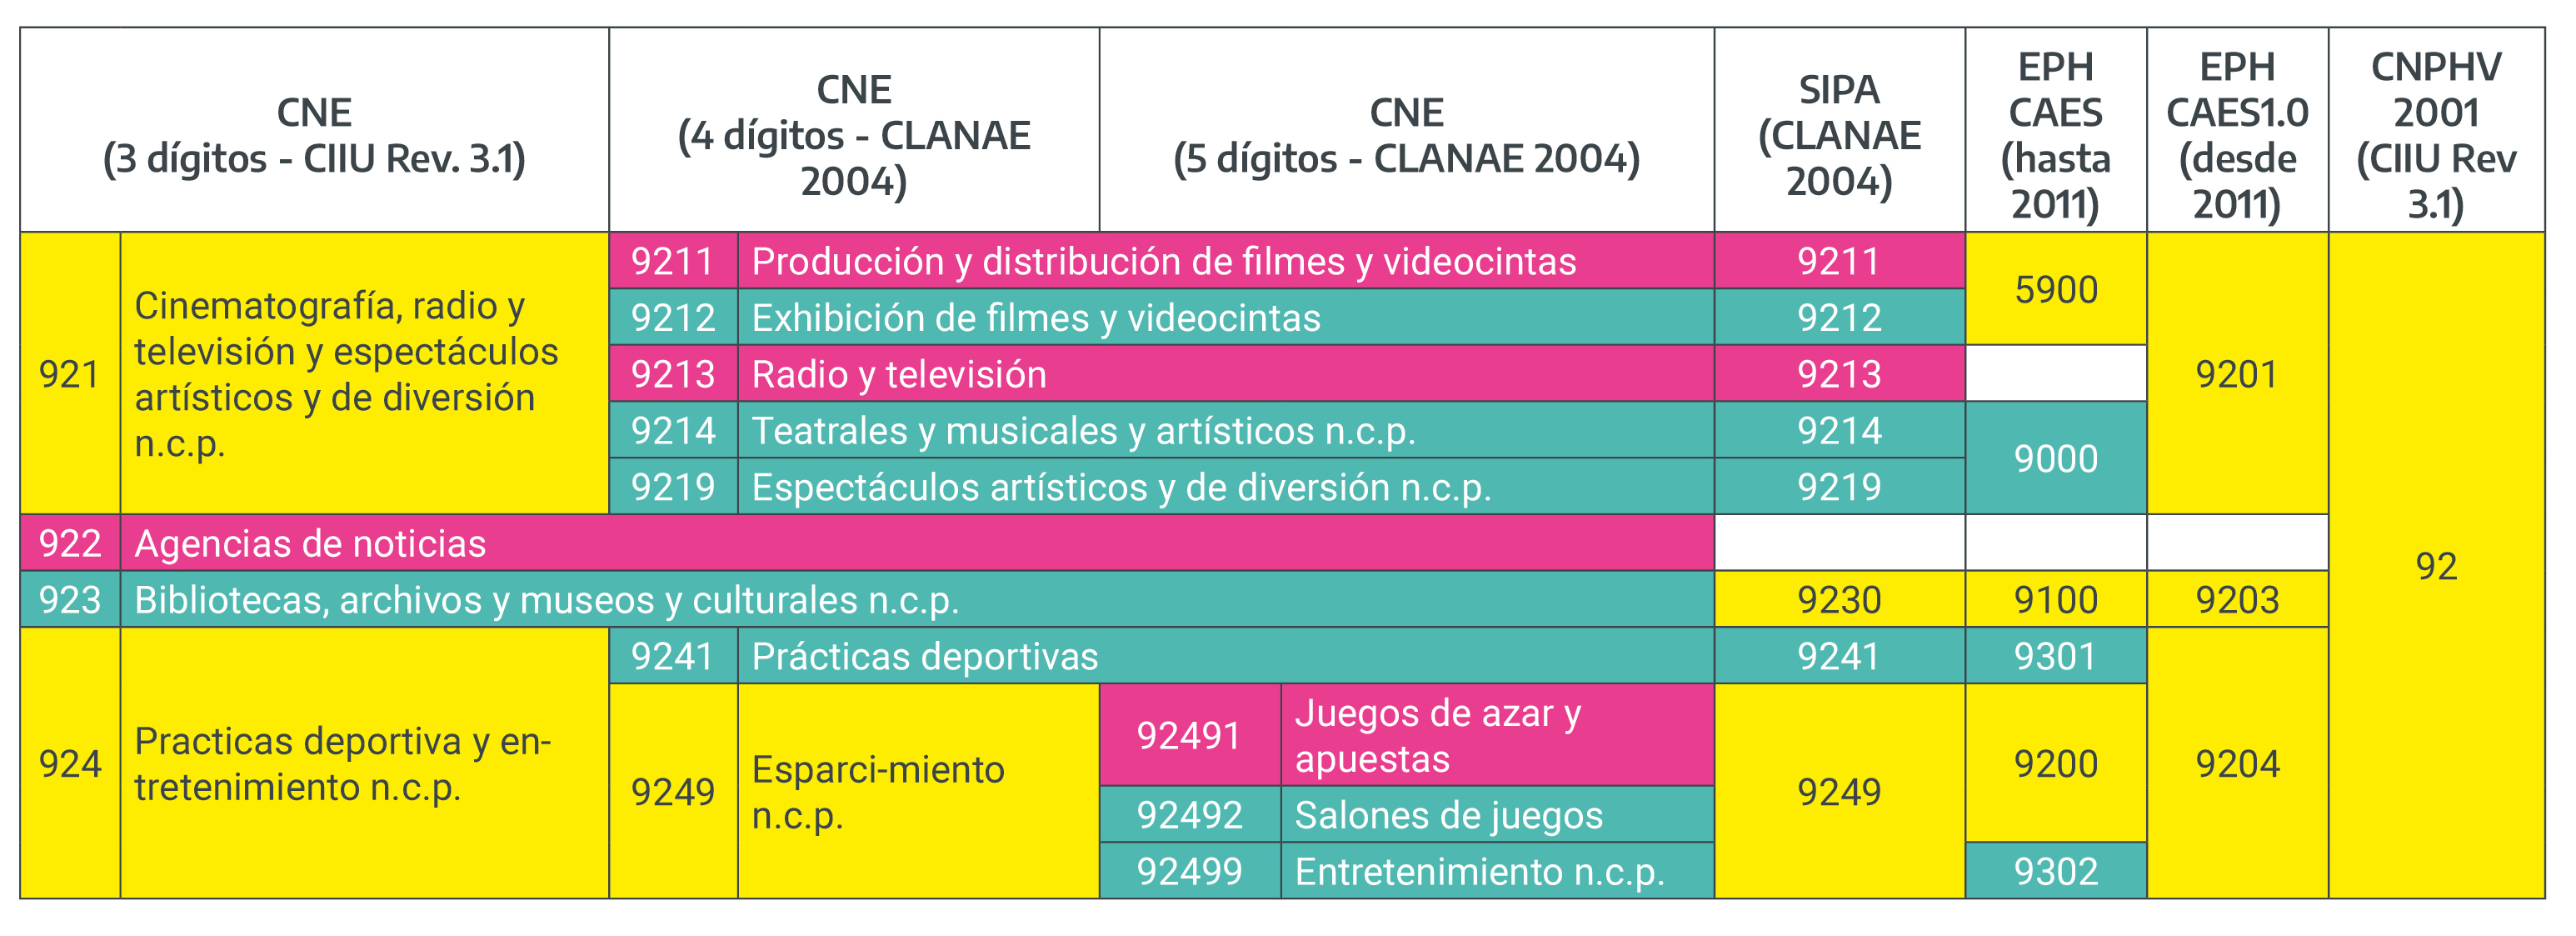
\includegraphics[width=1\linewidth]{imagenes/figura3.11} 

}

\caption{ Servicios de Esparcimiento, Culturales y  Deportivos. Clasificación de actividades por fuente.}\label{fig:empleofuentes11}
\end{figure}

\hypertarget{acceso-a-la-informaciuxf3n-presentada}{%
\section{Acceso a la información presentada}\label{acceso-a-la-informaciuxf3n-presentada}}

Todas las fuentes de información aquí descriptas se encuentran disponibles al público en general, a excepción del CNE 04/05, que publica cuadros a nivel provincial por ramas agrupadas de actividad (v.g. ``Hoteles y Restaurantes'').

A continuación se especifica la ubicación en Internet de cada fuente, indicando el tipo de información disponible.

Cabe señalar que junto con la información podrán encontrarse los documentos metodológicos básicos.

\href{https://www.indec.gob.ar/indec/web/Institucional-Indec-BasesDeDatos-1}{\textbf{EPH y EPH total urbano}} Las bases de datos se brindan en formato TXT a partir de 2016 y en SPSS, Stata y DBF para los años previos.
Recordar que para la EPH existe una base trimestral, mientras que para la EPH total urbano -o EAHU para 2010-2014- sólo una base anual, que corresponde al tercer trimestre de cada año.

\href{https://www.indec.gob.ar/indec/web/Nivel3-Tema-2-41}{\textbf{CNPVH}}. Para los censos de 2001 y 2010 se puede utilizar (en línea) el programa REDATAM, que permite procesar la información de manera sencilla.

\href{https://sitioanterior.indec.gob.ar/cne2005_index.asp}{\textbf{CNE}} Tablas (formato Excel) para el total país y para cada provincia por sector de actividad económica.

\href{https://www.trabajo.gob.ar/estadisticas/oede/estadisticasregionales.asp}{\textbf{SIPA-MTYEySS}} se presenta una conjunto de tablas con información provincial en formato Excel para descargar, entre las que figura la serie trimestral de empleo registrado por rama de actividad a cuatro dígitos y, en algunas ramas como Servicio de transporte ferroviario, a 3 dígitos.

\hypertarget{ejemplos-de-utilizaciuxf3n-de-las-fuentes}{%
\section{Ejemplos de utilización de las fuentes}\label{ejemplos-de-utilizaciuxf3n-de-las-fuentes}}

\hypertarget{empleo-turuxedstico}{%
\subsection{Empleo turístico}\label{empleo-turuxedstico}}

A modo de ejemplo de uso de algunas de las fuentes presentadas en las secciones precedentes, se ilustran posibles aplicaciones para la medición del empleo provincial en ramas turísticas, teniendo en cuenta los lineamientos conceptuales de los capítulos anteriores. Se hará énfasis en las fuentes disponibles con actualizaciones recientes, con el objetivo de tener un acercamiento más actual a la información de empleo en el sector. En este sentido, las fuentes que se actualizan de manera trimestral y contienen información relativa al empleo en ramas turísticas son la EPH y las estadísticas de empleo registrado del OEDE-MTEySS a partir del SIPA. En el caso de la primera, debe tenerse en cuenta, como se mencionó anteriormente, que se trata de una encuesta probabilística, sujeta al margen de error estadístico. Por este motivo, teniendo en cuenta que el diseño de la encuesta no asegura la robustez de las estimaciones con apertura sectorial y geográfica, los resultados deben tomarse con cautela y, preferentemente, elegir un agrupamiento de trimestres que permita tener una cantidad de casos muestrales significativa. A esto se suma el hecho de que la cobertura geográfica de la EPH es de 31 aglomerados urbanos, y no de las provincias en su conjunto. Puede complementarse el análisis con la extensión de la cobertura de la EPH total urbano, únicamente para los terceros trimestres del año. La ventaja de esta fuente de información, como se ha mencionado, es que incluye a todas las categorías de ocupados: asalariados- con y sin aportes y/o descuento jubilatorio- e independientes -patrón o cuenta propia-.

\begin{figure}

{\centering 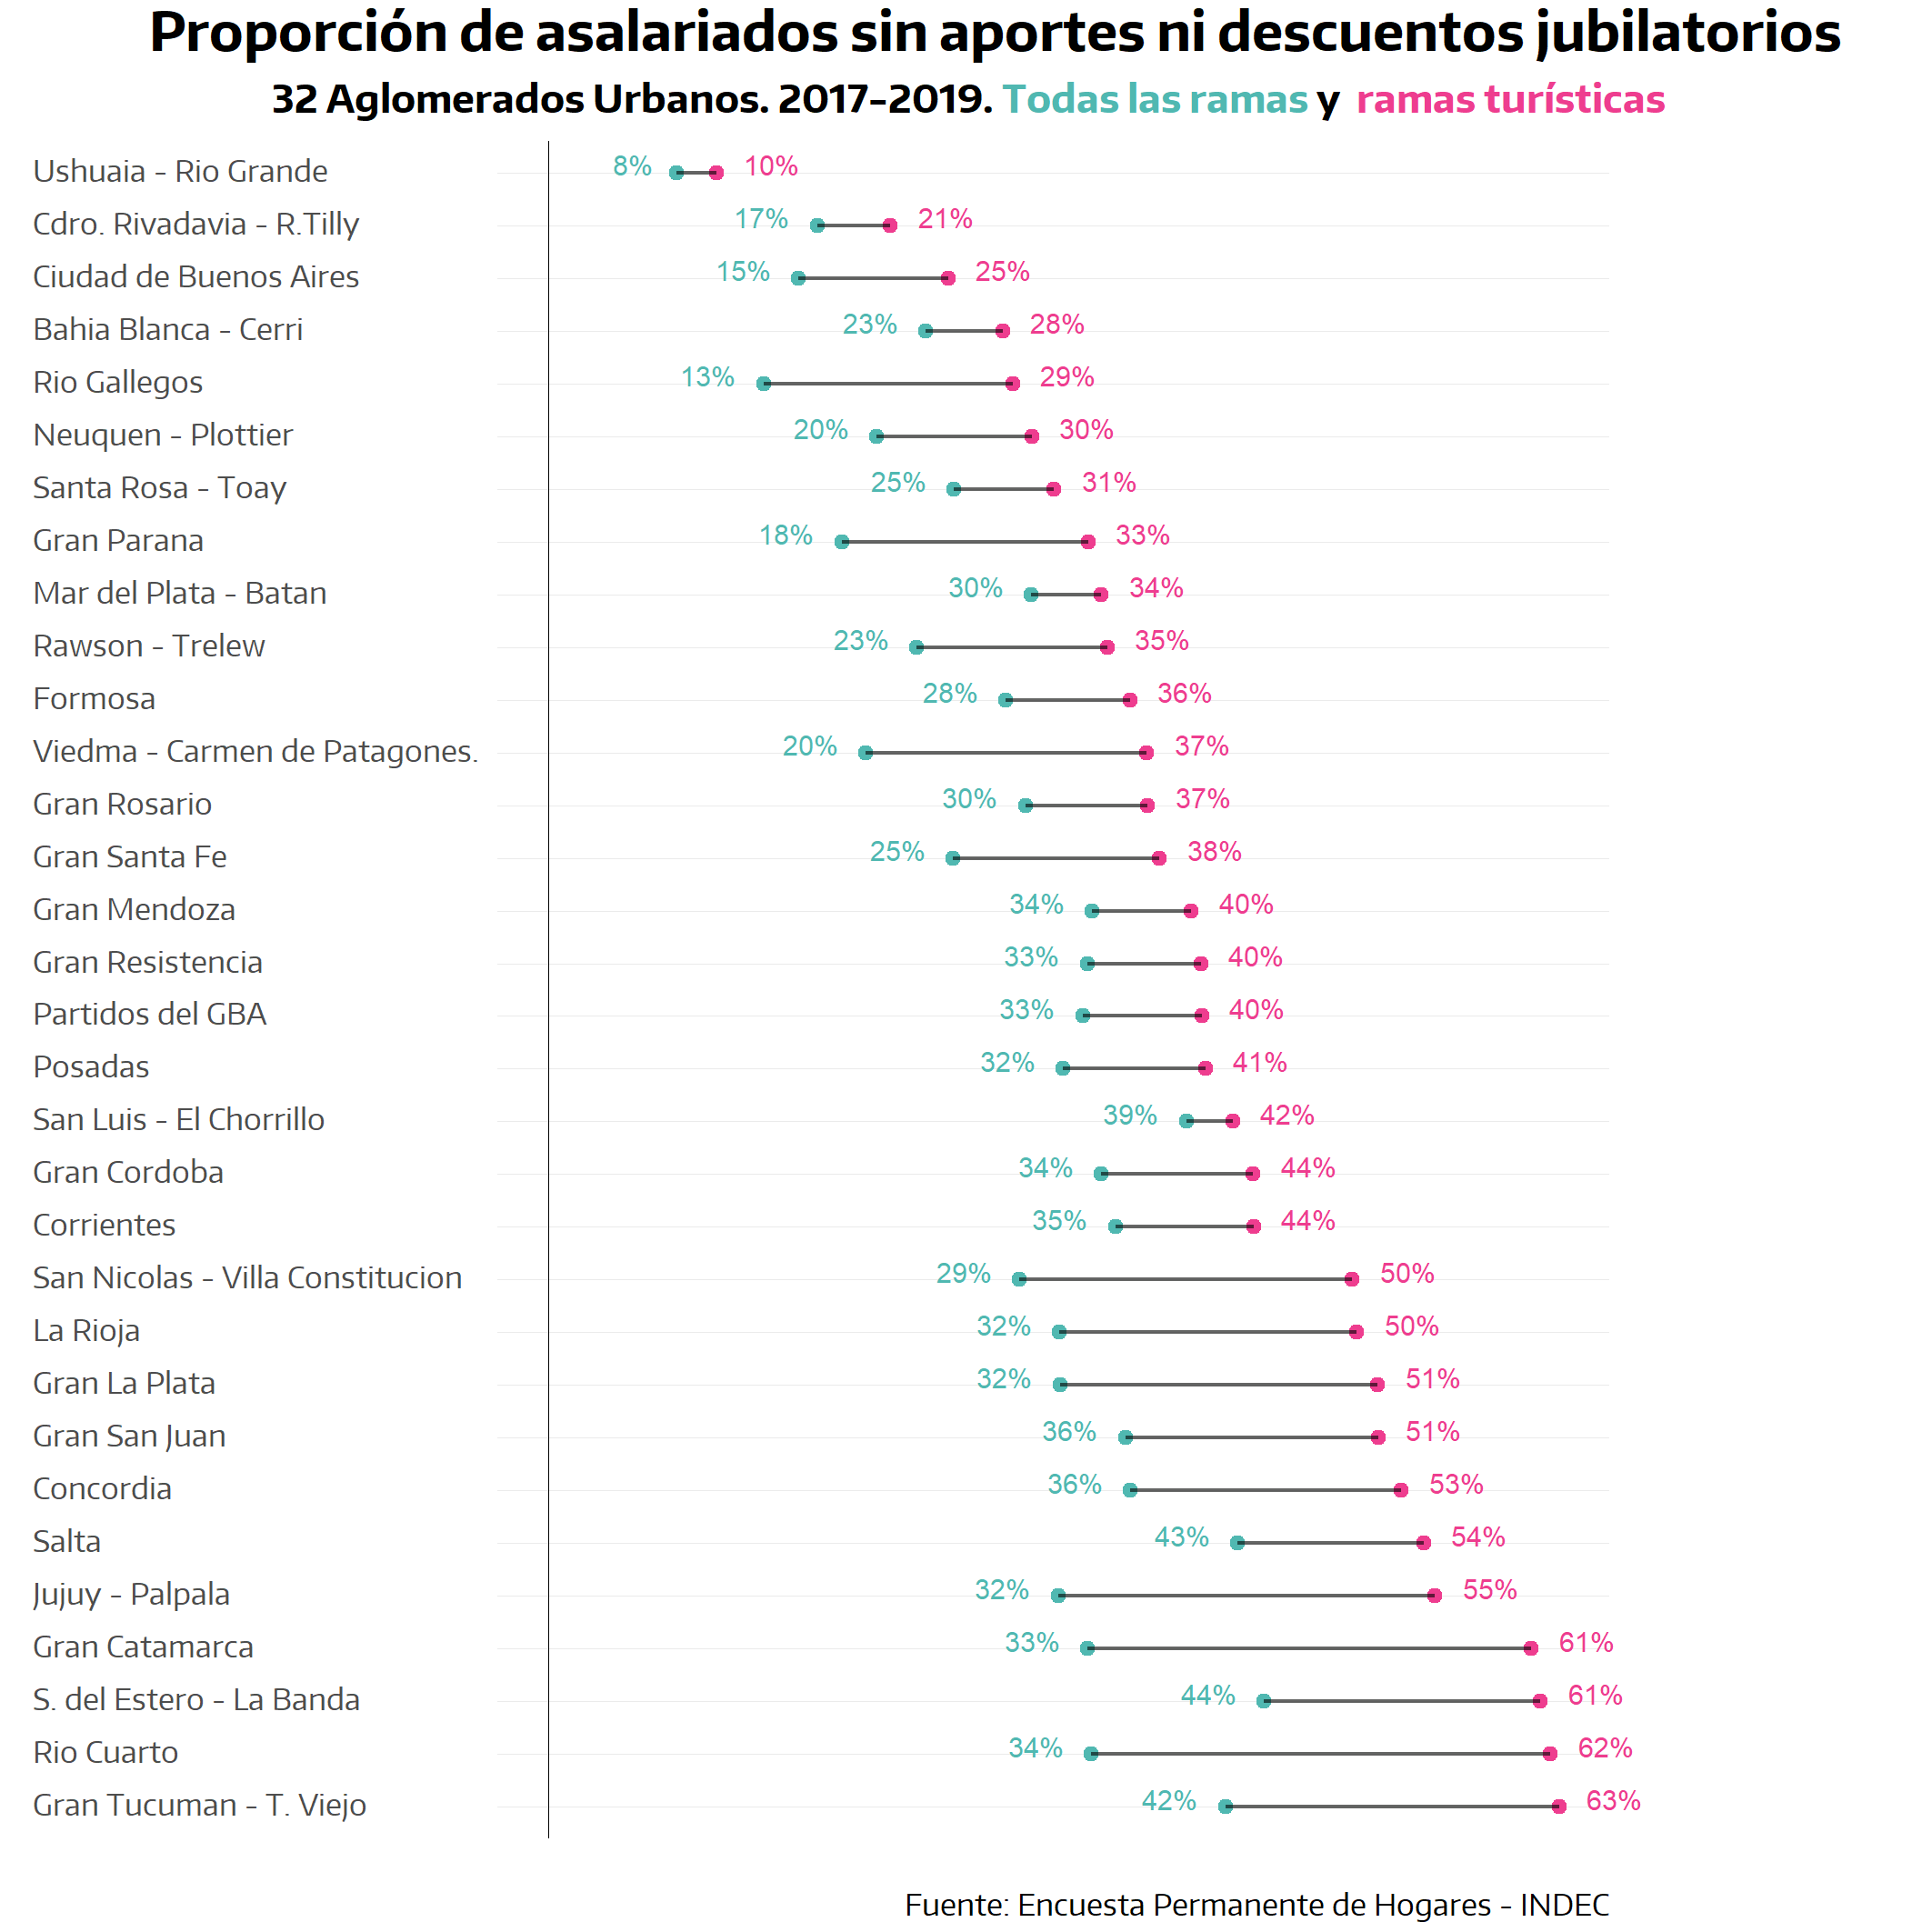
\includegraphics[width=1\linewidth]{imagenes/empleo eph} 

}

\caption{Tasa de informalidad para ramas características y todas las ramas.}\label{fig:empleoeph}
\end{figure}

La otra fuente actualizada para medir el empleo en ramas características del turismo es la publicación trimestral de los asalariados registrados por rama de actividad a 4 dígitos del OEDE-MTEySS a partir del SIPA. Al provenir de un registro administrativo, no está sujeta a errores de muestreo y tiene cobertura provincial\footnote{La información publicada, en el caso de la provincia de Buenos Aires, está dividida en GBA y Resto de Buenos Aires. En esta sección se sumaron ambas regiones para obtener el total de la provincia}. Una desventaja de esta información reside en que algunas ramas se encuentran abiertas a 3 dígitos, por ejemplo ``Servicios de transporte ferroviario'' se encuentra a 3 dígitos de apertura (rama 601), por lo que incluye servicio de carga y pasajeros. Sucede lo mismo con los transportes marítimo, fluvial y aéreo. El transporte automotor se encuentra a 4 dígitos, por lo que permite la separación de carga y pasajeros (rama 6022) pero no distinguir el transporte de pasajeros urbano e interurbano.
Asimismo, el origen de la información implica que no se incluyan trabajadores no registrados ni independientes. El siguiente gráfico muestra los trabajadores registrados por provincia, promediando los 4 trimestres de 2019, para todas las ramas y para las ramas turísticas.

\begin{center}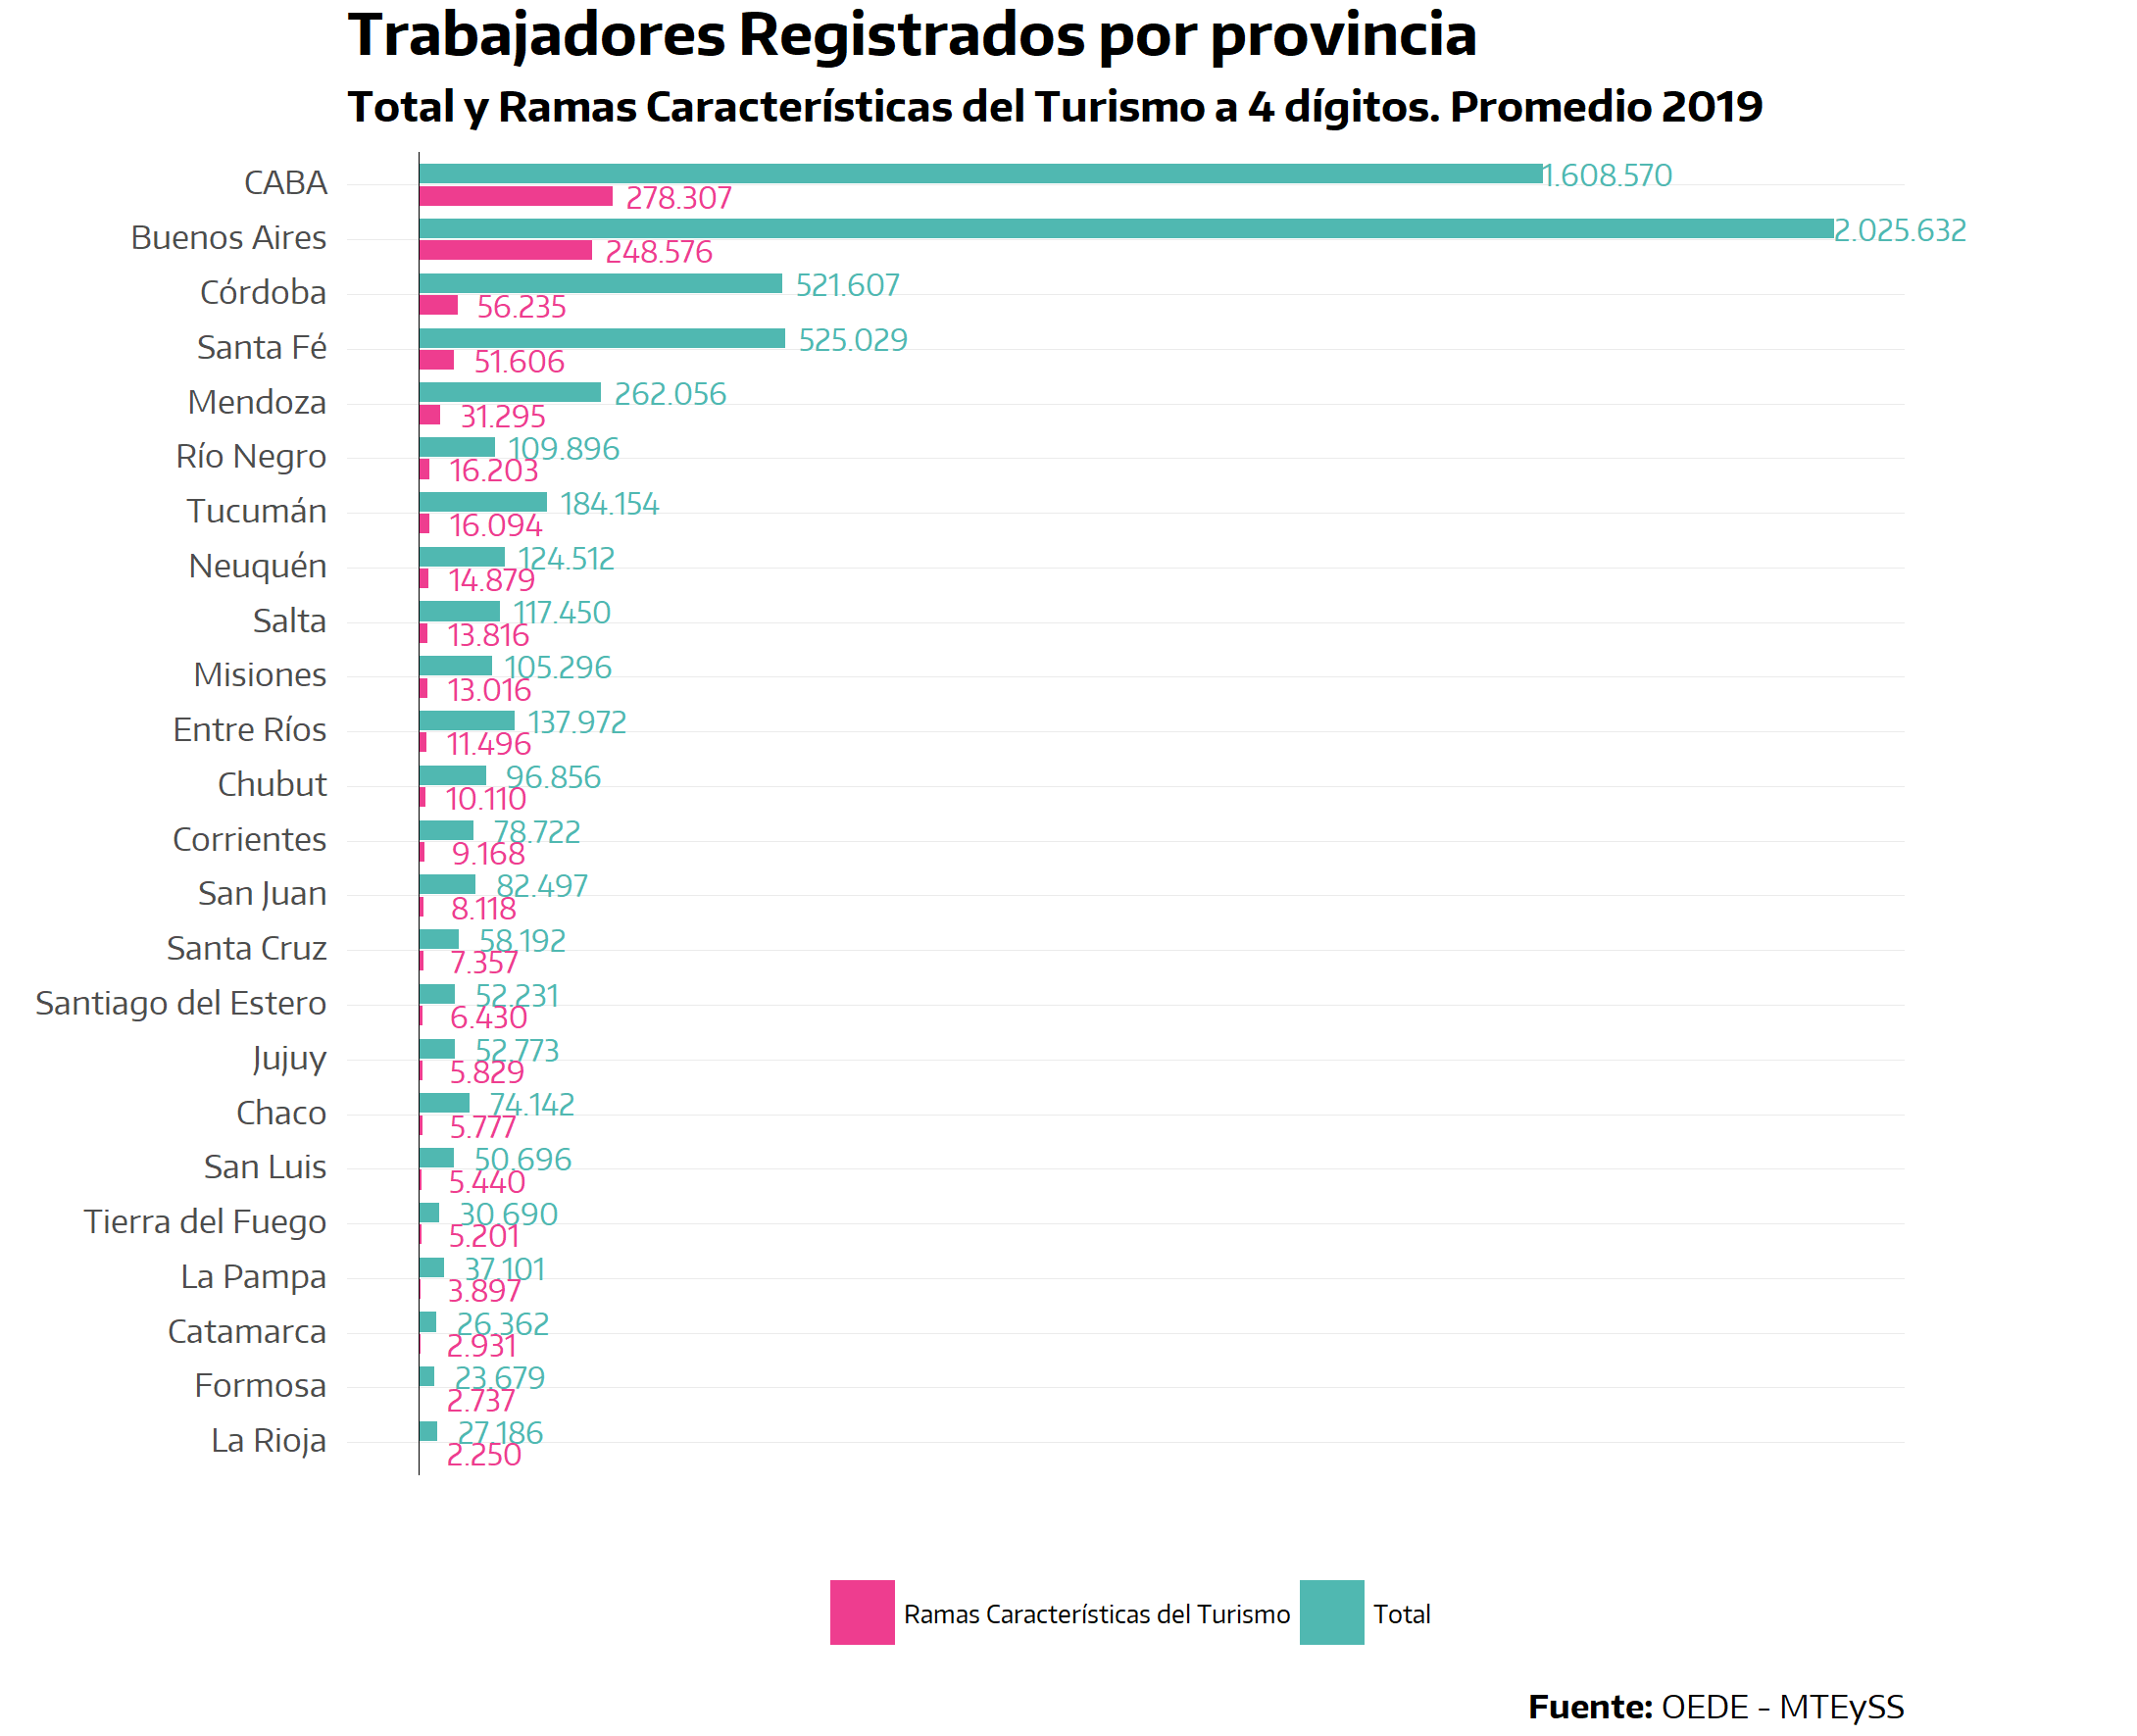
\includegraphics[width=1\linewidth]{imagenes/empleo.prov} \end{center}

A continuación, se muestra la participación de las ramas turísticas en el total del empleo registrado, para el mismo período de medición.

\begin{center}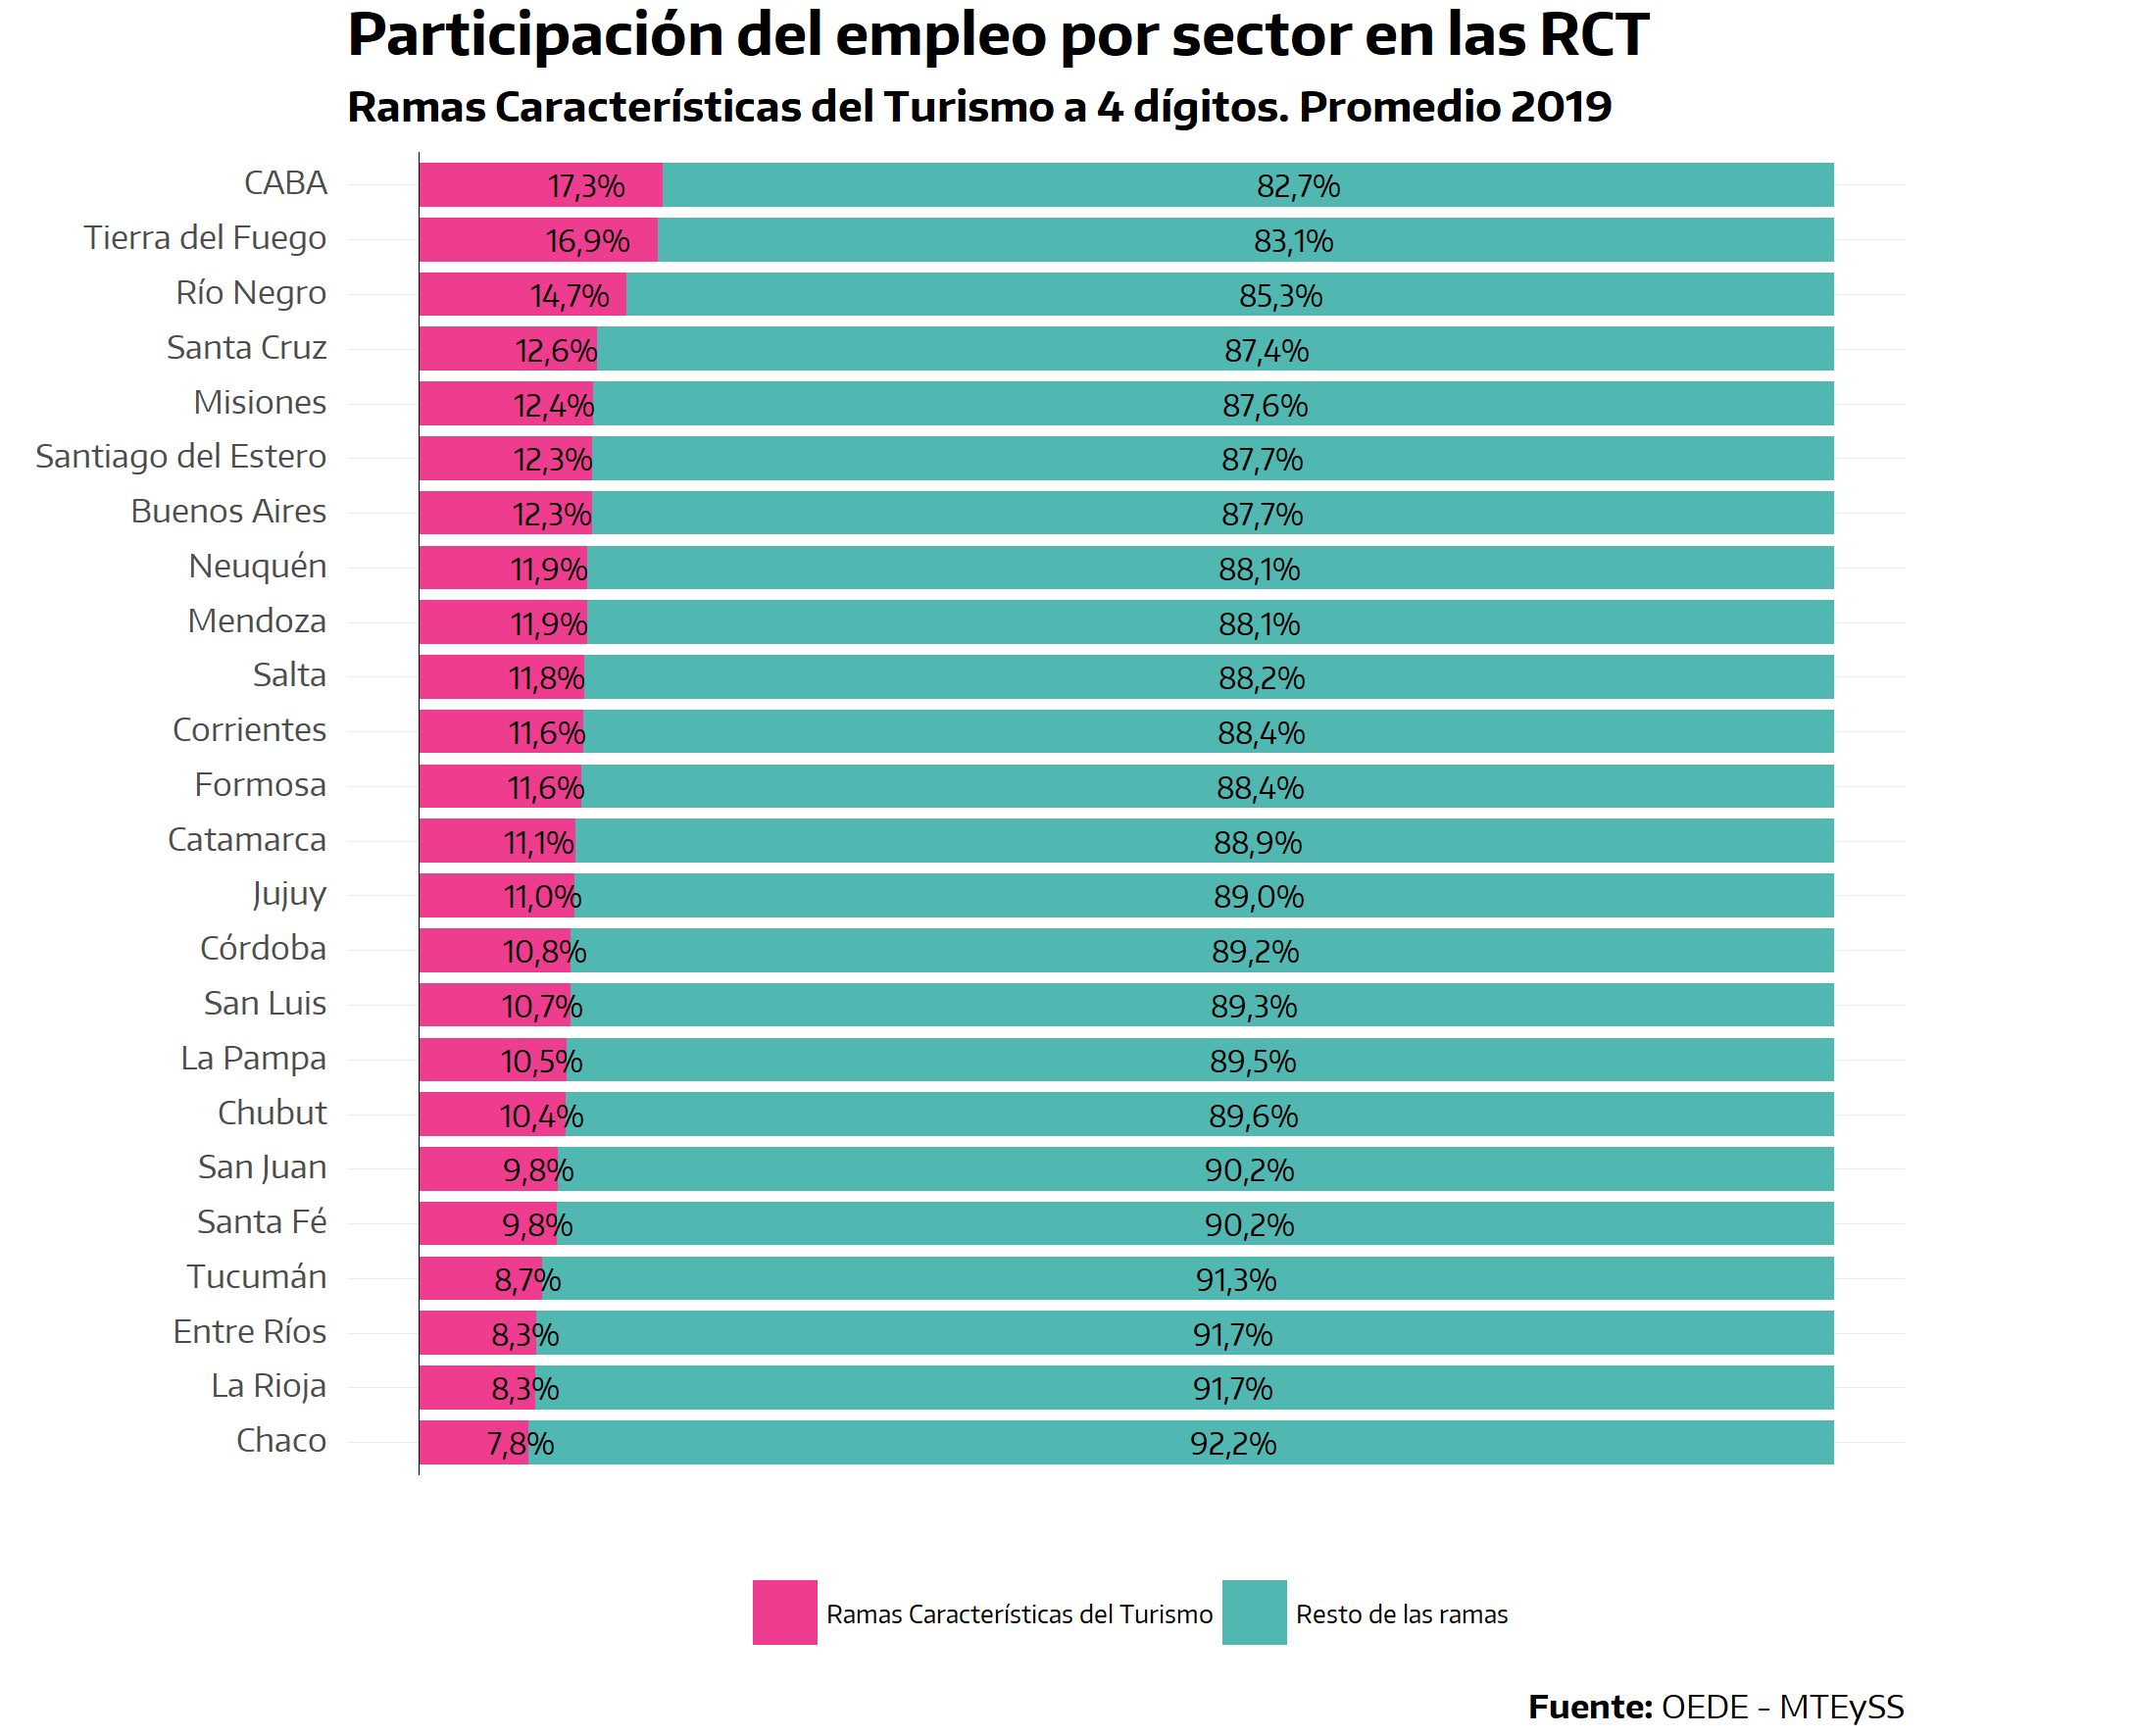
\includegraphics[width=1\linewidth]{imagenes/empleo.prov.part} \end{center}

El siguiente gráfico muestra la participación de cada categoría dentro del empleo en ramas características:

\begin{center}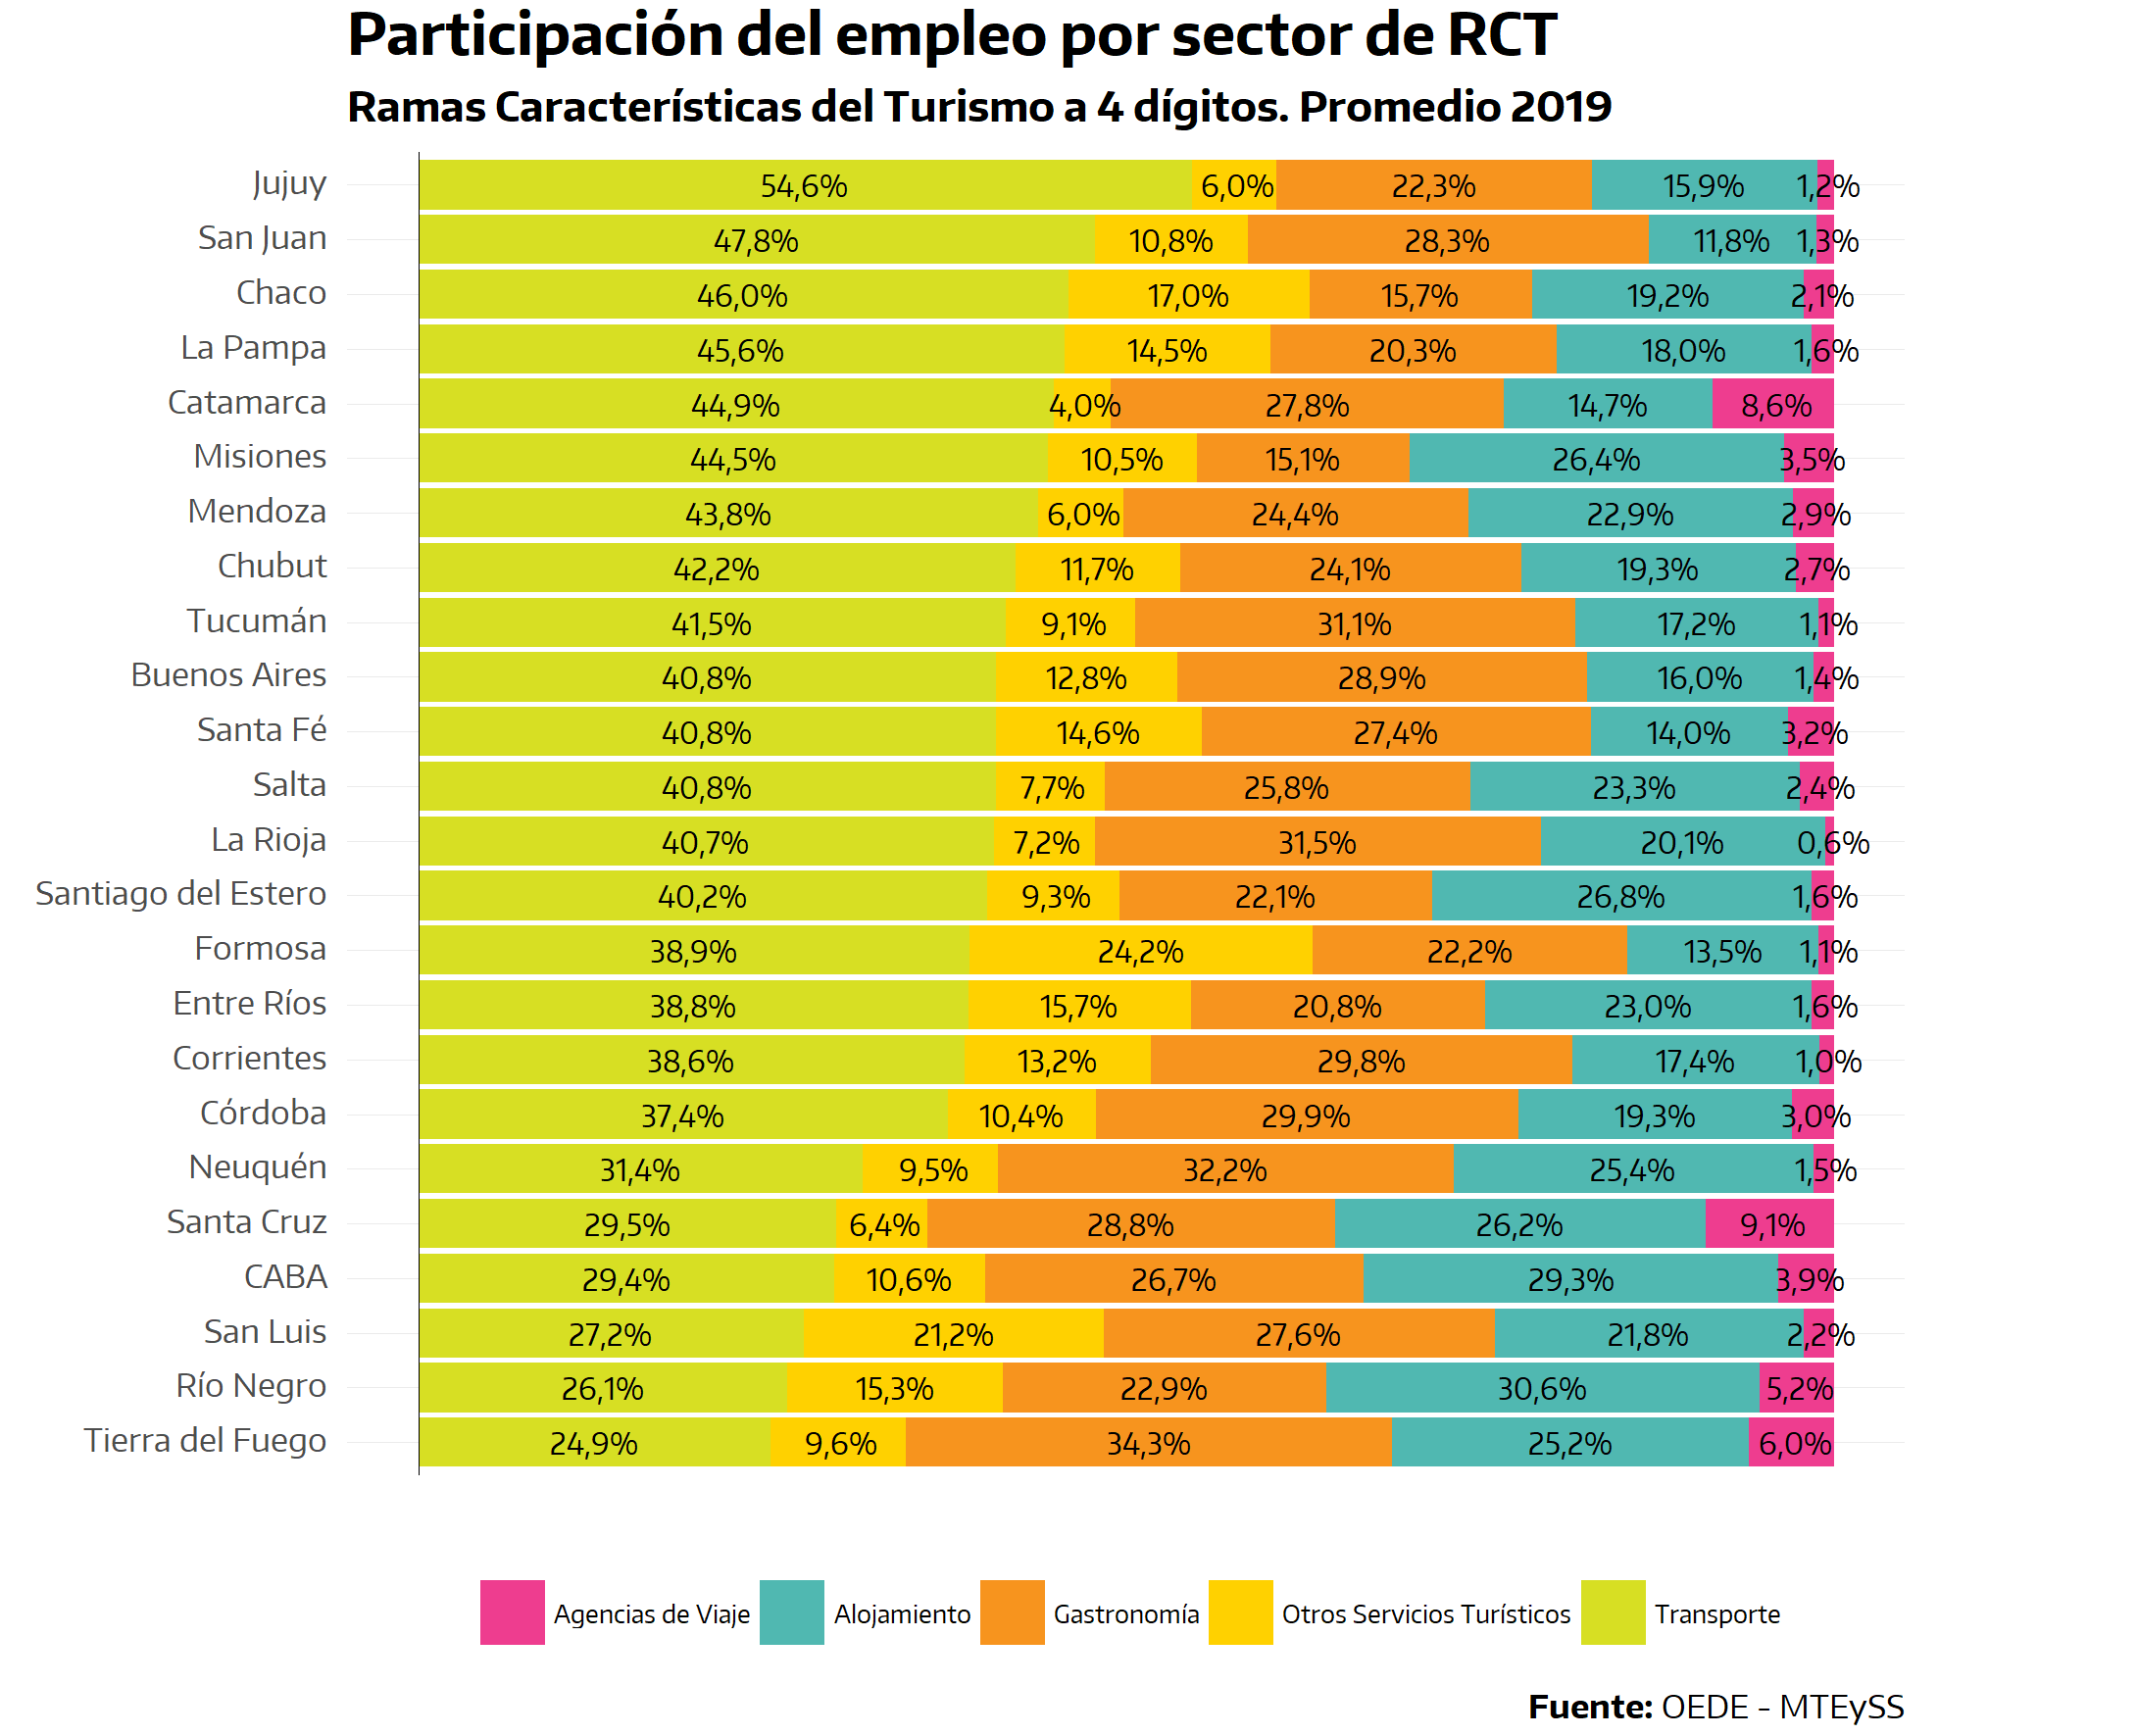
\includegraphics[width=1\linewidth]{imagenes/empleo.prov.part.agrup} \end{center}

\hypertarget{bibliografuxeda}{%
\chapter*{\texorpdfstring{\textbf{Bibliografía}}{Bibliografía}}\label{bibliografuxeda}}
\addcontentsline{toc}{chapter}{\textbf{Bibliografía}}

\hypertarget{refs}{}
\begin{CSLReferences}{1}{0}
\leavevmode\vadjust pre{\hypertarget{ref-scn2008}{}}%
Fondo Monteario Internacional, Organización de Cooperación y. Desarrollo Económico, Comisión Europea, y Banco Mundial (2016): \emph{Sistema de Cuentas Nacionales 2008}, Nueva York, ONU, \textless{}\url{https://unstats.un.org/unsd/nationalaccount/docs/sna2008spanish.pdf}\textgreater.

\leavevmode\vadjust pre{\hypertarget{ref-clanae04}{}}%
INDEC (2004): \emph{Clasificador Nacional de Actividades Económicas 2004 (CLANAE 2004)}, \textless{}\url{https://www.indec.gob.ar/ftp/cuadros/menusuperior/clasificadores/clanae_2004_19.pdf}\textgreater.

\leavevmode\vadjust pre{\hypertarget{ref-clanae10}{}}%
INDEC (2010): \emph{Clasificador Nacional de Actividades Económicas 2010 (CLANAE 2010)}, \textless{}\url{https://www.indec.gob.ar/micro_sitios/clanae/index3.asp}\textgreater.

\leavevmode\vadjust pre{\hypertarget{ref-mariscal2005}{}}%
Mariscal Galeano, Adela (2005): \emph{Mercado de trabajo y turismo en Andalucía actividad, ocupación y paro (1990-2003)}, Sevilla, Consejería de Turismo, Comercio y Deporte, \textless{}\url{https://datos.bne.es/edicion/bimo0002088698.html}\textgreater.

\leavevmode\vadjust pre{\hypertarget{ref-mintur2007}{}}%
Ministerio de Turismo y Deportes (2007): \emph{El empleo en ramas características del turismo en Argentina}, Buenos Aires, Ministerio de Turismo y Deportes, \textless{}\url{https://www.yvera.tur.ar/estadistica/}\textgreater.

\leavevmode\vadjust pre{\hypertarget{ref-oitconferencia14}{}}%
Oficina Internacional del Trabajo (2014): \emph{La transición de la economía informal a la economía formal}, Ginebra, OIT, \textless{}\url{https://www.ilo.org/wcmsp5/groups/public/---ed_norm/---relconf/documents/meetingdocument/wcms_218350.pdf}\textgreater.

\leavevmode\vadjust pre{\hypertarget{ref-cstrmc2008}{}}%
Oranización Mundial de Tursimo, Comisión Europea, Naciones Unidas, y Organización de Cooperación y Desarrollo Económico (2008): \emph{Cuenta satélite de turismo: Recomendaciones sobre el marco conceptual}, Luxemburgo/Madrid/París/Nueva York, ONU, \textless{}\url{https://www.e-unwto.org/doi/book/10.18111/9789213612392}\textgreater.

\leavevmode\vadjust pre{\hypertarget{ref-ciiurev3_1}{}}%
Organización de las Naciones Unidas (2005): \emph{Clasificación Industrial Internacional Uniforme de todas las actividades económicas (CIIU), Revisión 3.1}, Nueva York, ONU, \textless{}\url{https://unstats.un.org/unsd/classifications/Econ/Download/In\%20Text/ISIC31_Spanish.pdf}\textgreater.

\leavevmode\vadjust pre{\hypertarget{ref-ciiurev4}{}}%
Organización de las Naciones Unidas (2009): \emph{Clasificación Industrial Internacional Uniforme de todas las actividades económicas (CIIU), Revisión 4}, Nueva York, ONU, \textless{}\url{https://unstats.un.org/unsd/publication/seriesm/seriesm_4rev4s.pdf}\textgreater.

\leavevmode\vadjust pre{\hypertarget{ref-oit2004}{}}%
Organización Internacional del Trabajo (2004): \emph{Introducción a las Estadísticas Laborales de Turismo}, Ginebra, OIT, \textless{}\url{https://webunwto.s3-eu-west-1.amazonaws.com/imported_images/25994/ilo_b_sp.pdf}\textgreater.

\leavevmode\vadjust pre{\hypertarget{ref-riet2008}{}}%
Organización Mundial del Turismo, Naciones Unidas y (2010): \emph{Recomendaciones internacionales para estadísticas de turismo 2008}, Madrid/Nueva York, ONU, \textless{}\url{https://unstats.un.org/unsd/publication/seriesm/seriesm_83rev1s.pdf}\textgreater.

\end{CSLReferences}

\end{document}
